\documentclass[oneside,12pt]{book}
\usepackage[utf8]{inputenc}
\usepackage{standalone}
\usepackage[margin=2.5cm]{geometry}
\usepackage{graphicx}
\usepackage{hyperref}
\usepackage{lmodern}
\usepackage{float}
\usepackage[spanish]{babel}
\usepackage{csquotes}
\usepackage[figurename=Ilustración]{caption}
\usepackage[numbers]{natbib}
\usepackage{ragged2e}
\usepackage{array}
\usepackage{multirow}
\usepackage{parskip}
\usepackage{listings}
\usepackage{epigraph}
\usepackage{lipsum} % Texto de relleno en plantilla
\usepackage{subcaption}
\usepackage{amssymb}

\usepackage{algorithm}
\usepackage{algpseudocode}

% Glosario de términos - BEGIN
\usepackage{glossaries}
\makeglossaries\newglossaryentry{timple}
{
    name=timple,
    description={Pequeño instrumento de cinco cuerdas utilizado principalmente para el acompañamiento de canciones folkloricas en las Islas Canarias}
}

\newglossaryentry{feedback}
{
    name=feedback,
    description={Comentario o sugerencia de un usuario}
}

\newglossaryentry{notación musical}
{
    name=notación musical,
    description={Sistema de escritura utilizado para representar gráficamente una pieza musical}
}

\newglossaryentry{notación latina}
{
    name=notación latina,
    description={Notación musical para nombrar las notas musicales mediante las silabas do, re, mi, fa, sol, la y si}
}

\newglossaryentry{notación anglosajona}
{
    name=notación anglosajona,
    description={Notación musical para nombrar las notas musicales mediante las vocales C, D, E, F, G, A y B}
}

\newglossaryentry{escala musical}
{
    name=escala musical,
    description={Conjunto de sonidos ordenados para formar una secuencia de notas musicales}
}

\newglossaryentry{tónica}
{
    name=tónica,
    description={Nota cabecera de una escala}
}

\newglossaryentry{semitono}
{
    name=semitono,
    description={Distancia mínima entre dos notas}
}

\newglossaryentry{tono}
{
    name=tono,
    description={Equivalente a dos semitonos}
}


\newglossaryentry{octava}
{
    name=octava,
    description={Secuencia que forman las notas do, re, mi, fa, sol, la, si, do}
}

\newglossaryentry{acorde}
{
    name=acorde,
    description={Conjunto de tres o mas notas diferentes que en su reproducción constituyen una unidad armónica}
}

\newglossaryentry{cualidad}
{
    name=cualidad,
    description={Intervalo de semitonos que definen la construcción de un acorde}
}

\newglossaryentry{progresión}
{
    name=progresión,
    description={Sucesión de acordes}
}

\newglossaryentry{transposición}
{
    name=transposición,
    description={Incremento o decremento de los índices de las notas que conforman un acorde}
}

\newglossaryentry{afinación}
{
    name=afinación,
    description={En instrumentos de cuerda pulsada, acción de tensar una cuerda para obtener una nota}
}

\newglossaryentry{punteo}
{
    name=punteo,
    description={En instrumentos de cuerda pulsada, técnica que consiste en tocar piezas musicales tocando notas de forma individual o combinada}
}

\newglossaryentry{rasgueo}
{
    name=rasgueo,
    description={En instrumentos de cuerda pulsada, técnica que consiste en tocar distintas cuerdas utilizando uno o varios dedos, en forma de barrido}
}

\newglossaryentry{cuerda al aire}
{
    name=cuerda al aire,
    description={Pulsado de una cuerda sin presionar ningun traste}
}

\newglossaryentry{traste}
{
    name=traste,
    description={Tira metálica perpendicuar al mástil de un instrumento de cuerda pulsada}
}

\newglossaryentry{tablatura}
{
    name=tablatura,
    description={Notación musical para la representación gráfica a través de una tabla cuyas lineas horizontales equivalen a cuerdas y los números a los trastes}
}

\newglossaryentry{diagrama de acordes}
{
    name=diagrama de acordes,
    description={Notación musical para la representación de acordes sobre texto acompañados de un diagrama en forma de tabla cuyas lineas verticales equivalen a cuerdas y horizontales a trastes}
}

\newglossaryentry{cejilla}{
    name=cejilla,
    description={Utilizacion de un mismo dedo para la pulsación de varias cuerdas en un mismo traste}
}

\newglossaryentry{mock}
{
    name=mock,
    description={Un \textit{mock} es un objeto simulado que imita el comportamiento de un componente externo, útil para la ejecución de pruebas donde se pretende simular componentes externos.}
}
% Glosario de términos - END

%\usepackage{fancyhdr}
\usepackage{geometry}
\usepackage{color}\usepackage{graphicx,xcolor}

\renewcommand{\lstlistingname}{Algoritmo}
%\renewcommand{\lstlistlistingnam%e}{Índice de~\lstlistingname s}

\floatname{algorithm}{Algoritmo}
\renewcommand{\listalgorithmname}{Índice de~{\lstlistingname}s}


\lstset{
        basicstyle=\fontsize{7}{11}\ttfamily,
        language=Java,
        captionpos=b,
}

\usepackage{titlesec}
\setcounter{secnumdepth}{3}
\titleformat{\chapter}[display]
{\normalfont\huge\bfseries}{\chaptertitlename\ \thechapter}{20pt}{\Huge}

\urlstyle{same}
\title{Aplicación web para la creación, difusión y práctica de canciones para el timple}
\author{Chamil José Cruz Razeq}
\date{Curso 2025~-~2026}
\renewcommand{\contentsname}{Contenido}
%\renewcommand{\figurename}{Ilustración}
\addto\captionsspanish{%
  \renewcommand{\figurename}{Figura}%
}

\newcommand{\figref}[1]{(véase Figura~\ref{#1})}
\newcommand{\tabref}[1]{(véase Cuadro~\ref{#1})}



\usepackage{pifont}
%\renewcommand\labelitemi{\ding{52}}

\renewcommand{\arraystretch}{1.5}

\begin{document}
%\maketittle
\begin{titlepage}

\begin{center}

\vspace*{0.25in}
\begin{figure}[htb]
\begin{center}

\includegraphics[width=15cm]{Ilustraciones/NuevoLogoEII.png}
%
\includegraphics[width=15cm]{Ilustraciones/LogoEII.jpg}
%
\includegraphics[width=20cm]{Ilustraciones/Logo_EII+ULPGC.png}
\end{center}
\end{figure}

\vspace*{0.25in}
\vspace*{0.25in}
\begin{Huge}
    \textbf{Trabajo de Fin de Grado} \\
\end{Huge}
\vspace*{0.5in}

\noindent\hfil\rule{17cm}{0.2mm}\hfil\\

\vspace*{0.1in}
\begin{Huge}
    \textbf{Aplicación web para la creación, difusión y práctica de canciones para el timple} \\
\end{Huge}
\vspace*{0.3in}
\begin{large}
TITULACIÓN:~Grado en Ingeniería Informática \\
\vspace*{0.1in}
AUTOR:~Chamil José Cruz Razeq\\
\end{large}
\vspace*{0.3in}
\noindent\hfil\rule{17cm}{0.2mm}\hfil\\
\vspace*{0.1in}
\begin{large}
TUTORIZADO POR:\\
Francisco Alexis Quesada Arencibia\\
\end{large}
\vspace{0.5cm}
CO-TUTORIZADO POR:\\
Mariam Quesada Ojeda\\
\vspace*{0.3in}
10/2025

\end{center}


\end{titlepage}


\input{TFT04C.tex}

\newpage
\pagenumbering{roman}
{\Large{\textbf{Agradecimientos}}}

\begin{flushright}
    {\setlength{\parskip}{8mm}
        \large{
            \textit{}
        }
    }
    
\end{flushright}

\clearpage
{\setlength{\parskip}{8mm}
{\huge{\textbf{Resumen}}}

{\large{

El \gls{timple} es un pequeño instrumento profundamente arraigado en la cultura de las Islas Canarias. A pesar de su relevancia en el folclore local, este nunca llegó a popularizarse al nivel de otros instrumentos como la guitarra o el ukelele. Esta situación se ve agravada por la escasez de recursos accesibles y gratuitos que faciliten su aprendizaje y práctica.

Este proyecto propone el desarrollo de una aplicación web orientada a la creación, difusión y práctica de canciones para timple. Para ello, la aplicación contará con un conjunto de herramientas para la creación y reproducción de canciones, páginas informátivas con utilidades para introducirse al instrumento y un espacio donde acceder a todos los recursos anteriores.

A lo largo del documento se expone de forma estructurada el proceso de desarrollo del proyecto, abarcando las fases de análisis, diseño, implementación, pruebas y despliegue, así como otros aspectos relevantes como la normativa y legislación, herramientas, metodología y planificación utilizadas.

}}

\newpage

{\huge{\textbf{Abstract}}}


{\large{

The \emph{\gls{timple}} is a small instrument deeply rooted in the culture of the  Canary Islands. Although relevant in local culture, it did not have the chance to be as popular as other instruments such as the guitar or ukulele. The lack of reachable and free resources for the learning and practice of the instrument made the situation even worse.

The aim of this project is to develop of a web application that facilitates the creation, destribution and practice of music for the \emph{timple}. To achieve this, the application counts with a set of tools for the creating and practicing of songs, informative pages with utilities that ease the first steps with the instrument, and an easy to access space to the resources mentioned.

Throughout this document you will follow the development of this project, getting through phases such as analysis, design, implementation, tests and deployment, as other relevant aspects such as normative and legilation, tools, methodology and planificacion used.

}

}}
\tableofcontents

%\addcontentsline{toc}{section}{Listings}
%\lstlistoflistings
\listofalgorithms\listoffigures\listoftables


\clearpage
\pagenumbering{arabic}

\chapter{Introducción}

Este capítulo describe apartados introductorios del proyecto: motivación, objetivos, aportaciones, competencias específicas, relación con los objetivos de desarrollo sostenible y la organización del documento.

\section{Motivación}
El timple es un pequeño instrumento de cuerda muy popular en el folclore de las Islas Canarias. Sin embargo, a diferencia de otros instrumentos como la guitarra o el ukelele, el timple no consiguió expandirse mas hallá de las fronteras insulares. Aunque podemos encontrar una comunidad en torno a este instrumento, la falta de recursos accesibles y gratuitos dificulta su aprendizaje y práctica, especialmente para aquellos que desean iniciarse en el instrumento.

Dada la popularidad de plataformas digitales diseñadas para otros instrumentos y la inexistencia de un espacio dedicado para el timple, surge la oportunidad de desarrollar una aplicación web que cubra esta necesidad, sirviendo como punto de encuentro para su comunidad, contribuyendo a la difusión y preservación de este instrumento tradicional.
\section{Objetivos}

El \textbf{objetivo principal} de este proyecto es el desarrollo de una aplicación web especificamente diseñada para el aprendizaje, práctica y difusión de canciones para timple.

La complejidad que conlleva la elaboración de un espacio digital de este tipo requiere de la definición de una serie de \textbf{objetivos específicos}:

\begin{itemize}
    \item \textbf{Disponibilidad de recursos didácticos}, en forma de páginas informativas con contenidos diseñados para iniciarse en el instrumento.
    \item \textbf{Publicación de canciones}, donde se mostrará información general de la pieza (autor, album, género...), letra y acordes.
    \item \textbf{Existencia de una biblioteca de canciones}, permitiendo la búsqueda y acceso a las canciones publicadas.
    \item \textbf{Creación de herramientas y utilidades}, como el autodesplazamiento, visualización de acordes, transposición automática, ajustes de visualización...
    \item \textbf{Comunidad digital}, a través de las publicaciones de usuarios, caja de comentarios, sistema de me gusta, perfiles…
\end{itemize}

\section{Principales aportaciones}
El desarrollo de este proyecto ofrece aportaciones en tres entornos: social y técnico.

\subsection{Social}

Dada la gran importancia cultural del timple, especialmente para la sociedad canaria, la ejecución de este proyecto resulta en un espacio dedicado a la comunidad del timplistas y todas aquellas personas interesadas en el mismo.

La aplicación web pone a disposición de los usuarios un amplio abanico de posibilidades: desde el aprendizaje a través de las páginas informativas, hasta la creación y publicación de canciones, así como el uso de herramientas para facilitar la práctica del instrumento.

Este espacio pone, mas cerca que nunca, el timple en manos de todo aquel que quiera tocarlo.

A nivel social podemos encontrar varias aportaciones.

En primer lugar, la existencia de este espacio promueve la difusión del propio instrumento, ayudando a preservar su legado cultural y a aumentar su popularidad entre nuevas generaciones y diferentes regiones geográficas.

En segundo lugar, la aplicación web ofrece a los usuarios recursos para el aprendizaje y práctica del timple, facilitando la accesibilidad al instrumento y fomentando su estudio.

En tercer lugar, la aplicación web fomenta la creación de contenido musical para el timple, facilitando a los usuarios la publicación y compartición de canciones.

En cuarto y último lugar, aunque ya existen comunidades de timplistas, este espacio digital puede servir como punto de encuentro para todos aquellos interesados en el instrumento, promoviendo la interacción y colaboración entre sus miembros.

\subsection{Técnico}
La principal aportación técnica de este proyecto es la creación de un espacio donde el timple sea el protagonista. Para ello, es necesario el desarrollo de utilidades adaptadas tanto a las singularidades técnicas del instrumento como a su contexto cultural. Dada la escasez de recursos y referencias digitales, la creación de esta aplicación web representa un importante desafío.

Actualmente existen espacios dedicados a la práctica de instrumentos como la guitarra y el ukelele. Estos ofrecen una experiencia adaptada a sus necesidades particulares, contando con grandes comunidades y en constante crecimiento a nivel internacional.


\section{Competencias específicas}
En conformidad con la \textbf{\emph{Memoria de Verificación del Título de Grado en Ingeniería Informática}} \cite{ulpgc_memoria2019}, se exponen a continuación las competencias específicas relacionadas con este proyecto.

\subsection{Competencias comunes a la rama informática}
\begin{itemize}
    \item \textbf{CI1~-~\emph{Capacidad para diseñar, desarrollar, seleccionar y evaluar aplicaciones y sistemas informáticos, asegurando su fiabilidad, seguridad y calidad, conforme a principios éticos y a la legislación y normativa vigente.}}

    Esta competencia se aborda en varios capítulos del proyecto, como;
    estado del arte, normativa y legislación, y tecnologías y herramientas.

    \item \textbf{CI2~-~\emph{Capacidad para planificar, concebir, desplegar y dirigir proyectos, servicios y sistemas informáticos en todos los ámbitos, liderando su puesta en marcha y su mejora continua y valorando su impacto económico y social.}}

    Se trabaja esta competencia durante todo el proyecto, comenzando por la selección de la metodología a utilizar, pasando por la planificación y terminando con la ejecución del proyecto.

    \item \textbf{CI3~-~\emph{Capacidad para comprender la importancia de la negociación, los hábitos de trabajo efectivos, el liderazgo y las habilidades de comunicación en todos los entornos de desarrollo de software.}}

    Podemos ver esta competencia reflejada tanto en el capítulo de estado del arte como en el desarrollo. Por un lado, a través de la investigación y análisis del contexto y alcance del proyecto, y por otro lado, a través del análisis de requisitos y diseño.
    
    \item \textbf{CI6~-~\emph{Conocimiento y aplicación de los procedimientos algorítmicos básicos de las tecnologías informáticas para diseñar soluciones a problemas, analizando la idoneidad y complejidad de los algoritmos propuestos.}}

    Se cubre esta competencia en el capítulo de desarrollo, específicamente en la construcción de un algoritmo que permite el cálculo de acordes.

    \item \textbf{CI7~-~\emph{Conocimiento, diseño y utilización de forma eficiente de los tipos y estructuras de datos más adecuados a la resolución de un problema.}}

    Queda demostrada en el capítulo de desarrollo, donde se diseñan e implementan estructuras de datos adaptadas a las características particulares de la funcionalidad en cuestión.

    \item \textbf{CI8~-~\emph{Capacidad para analizar, diseñar, construir y mantener aplicaciones de forma robusta, segura y eficiente, eligiendo el paradigma y los lenguajes de programación más adecuados.}}

    Esta competencia se desarrolla en el estado del arte, tecnologías y herramientas y desarrollo, donde se ejecutan los aspectos de análisis, selección de herramientas, diseño e implementación.

    \item \textbf{CI12~-~\emph{Conocimiento y aplicación de las características, funcionalidades y estructura de las bases de datos, que permitan su adecuado uso, y el diseño y el análisis e implementación de aplicaciones basadas en ellos.}}

    En el capítulo de desarrollo se expone el conocimiento, diseño e implementación de funcionalidades y bases de datos, vitales para la entrega de valor de la aplicación web al usuario.
    
    \item \textbf{CI16~-~\emph{Conocimiento y aplicación de los principios, metodologías y ciclos de vida de la ingeniería del software.}}

    Se justifica esta competencia a través de los capítulos de metodología y planificación, y desarrollo. A través de los anteriores, se selecciona y explica la metodología y planificación sobre la que se desarrollará el proyecto, además de la demostración de su correcta ejecución.
    
    \item \textbf{CI17~-~\emph{Capacidad para diseñar y evaluar interfaces persona computador que garanticen la accesibilidad y usabilidad a los sistemas, servicios y aplicaciones informáticas.}}

    Esta competencia se expone en los capítulos de estado del arte y desarrollo, evaluando las soluciones ya existentes y planteando nuevas propuestas para el diseño de experiencias e interfaces de usuario del proyecto.

    \item \textbf{CI18~-~\emph{Conocimiento de la normativa y la regulación de la informática en los ámbitos nacional, europeo e internacional.}}

    Se dedica un capítulo exclusivamente a la exposición de la normativa y legislación, además de una sección sobre licencias en el capítulo de tecnologías y herramientas.
    
\end{itemize}

\subsection{Competencias de tecnología específica}
\begin{itemize}    
    \item \textbf{TI6~-~\emph{Capacidad de concebir sistemas, aplicaciones y servicios basados en tecnologías de red, incluyendo Internet, web, comercio electrónico, multimedia, servicios interactivos y computación móvil.}}

    Esta competencia se materializa en el resultado final del proyecto, con la existencia de una aplicación web funcional.
    
\end{itemize}

\subsection{Competencia de trabajo de fin de grado}
\begin{itemize}
    \item \textbf{TFG~-~\emph{Ejercicio original a realizar individualmente y presentar y defender ante un tribunal universitario, consistente en un proyecto en el ámbito de las tecnologías específicas de la Ingeniería en Informática de naturaleza profesional en el que se sinteticen e integren las competencias adquiridas en las enseñanzas.}}

    Esta competencia se cumple con la realización integral del proyecto, que incluye tanto la aplicación desarrollada como el presente documento, reflejando la capacidad de síntesis e integración de las competencias adquiridas a lo largo del grado.

\end{itemize}

\section{Alineamiento con los objetivos de desarrollo sostenible}
En conformidad a los \textbf{\emph{Objetivos de Desarrollo Sostenible (ODS)}}~\cite{ODS2023} aprobados por los \emph{Estados Miembros} de las \emph{Naciones Unidas}, identificamos los siguientes ODS alineados con este proyecto~\tabref{tab:ODS}:

\begin{itemize}
    \item \textbf{Objetivo 5: Educación de Calidad -~\emph{Garantizar una educación inclusiva, equitativa y de calidad y promover oportunidades de aprendizaje durante toda la vida para todos.}~\cite{ods_educacion}} \\
    El desarrollo de este proyecto resulta en la existencia de un espacio digital que permite a cualquier persona, de forma gratuita y accesible, iniciarse en el instrumento, complementar su práctica, o colaborar con nuevas publicaciones.

    La capacidad de aprender, crear y difundir fomentan la retroalimentación del contenido de la aplicación, cuyo crecimiento servirá para atraer a nuevos usuarios interesados en el timple.
    
    \item \textbf{Objetivo 10: Reducción de las desigualdades -~\emph{Reducir la desigualdad en y entre los países.}~\cite{ods_desigualdad}} \\
    La naturaleza digital de la aplicación web, permite su disponibilidad en cualquier momento y lugar del planeta, acercando sus recursos y contenidos a cualquier usuario interesado.
    
    \item \textbf{Objetivo 11: Ciudades y comunidades sostenibles -~\emph{Lograr que las ciudades sean más inclusivas, seguras, resilientes y sostenibles.}~\cite{ods_ciudades}} \\
    La ya existente comunidad de timplistas puede encontrar un espacio donde complementar la enseñanza o práctica del instrumento, publicar material ya existente o simplemente formar parte de este espacio digital, creado especialmente para ellos.
    
    \item \textbf{Objetivo 17: Alianzas para lograr objetivos -~\emph{Revitalizar la Alianza Mundial para el Desarrollo Sostenible.}~\cite{ods_asociaciones}} \\
    La creación de recursos en la aplicación web depende, en un principio, de la colaboración de la ya existente comunidad de timplistas. A medida que la aplicación web se difunda y mas usuarios se inicien en el instrumento, mayor sera la posibilidad de que estos creen nuevos contenidos ampliando el catalogo y la variedad.
    
\end{itemize}

\begin{table}[H]
    \centering
    \caption{Grado de relación del TFT con los Objetivos de Desarrollo Sostenible}\label{tab:ODS}
    \scriptsize
    \begin{tabular}{lcccc}
        \hline
        \multirow{2}{*}{\centering\textbf{ODS}} & \multicolumn{4}{c}{\textbf{Grado de relación}} \\ 
        & No procede & Bajo & Medio & Alto \\ 
        \hline
        1 Fin de la pobreza & \ding{51} & & & \\
        2 Hambre cero & \ding{51} & & & \\
        3 Salud y bienestar & \ding{51} & & & \\
        4 Educación de calidad & & & \ding{51} & \\
        5 Igualdad de género & \ding{51} & & & \\
        6 Agua limpia y saneamiento & \ding{51} & & & \\
        7 Energía asequible y no contaminante & \ding{51} & & & \\
        8 Trabajo decente y crecimiento económico & \ding{51} & & & \\
        9 Industria, innovación e infraestructuras & \ding{51} & & & \\
        10 Reducción de las desigualdades & & & \ding{51} & \\ 
        11 Ciudades y comunidades sostenibles & & & \ding{51} & \\
        12 Producción y consumo sostenibles & \ding{51} & & & \\
        13 Acción por el clima & \ding{51} & & & \\
        14 Vida submarina & \ding{51} & & & \\
        15 Vida de ecosistemas terrestres & \ding{51} & & & \\
        16 Paz, justicia e instituciones sólidas & \ding{51} & & & \\
        17 Alianzas para lograr los objetivos & & & \ding{51} & \\ 
        \hline
    \end{tabular}
\end{table}

\section{Estructura del documento}

Este documento está organizado en diez capítulos, complementados por la bibliografía y los índices de contenidos, algoritmos, figuras y cuadros. A continuación se exponen brevemente los contenidos de cada capítulo.

\begin{itemize}
    \item \textbf{Capítulo 1~-~Introducción.} \\
    Este capítulo describe apartados introductorios del proyecto: motivación, objetivos, aportaciones, competencias específicas, relación con los objetivos de desarrollo sostenible y la organización del documento.
    
    \item \textbf{Capítulo 2~-~Metodología y planificación.} \\
    Este capítulo describe la metodología utilizada además de mostrar la planificación del proyecto.

    \item \textbf{Capítulo 3~-~Estado del Arte.} \\
    Este capítulo abarca aspectos como los fundamentos musicales necesarios para el desarrollo del proyecto, el estado actual, análisis de competencia y alcance del proyecto.

    \item \textbf{Capítulo 4~-~Normativa y legislación.} \\
    Este capítulo se centra en los aspectos legales que rodean al proyecto, así como la normativa y legislación vigente.

    \item \textbf{Capítulo 5~-~Tecnologías y herramientas.} \\
    Este capítulo expone las tecnologías y herramientas utilizadas durante el desarrollo del proyecto, así como las licencias de uso.
    
    \item \textbf{Capítulo 6~-~Desarrollo.} \\
    Este capítulo cubre el desarrollo, exponiendo cada incremento realizado para la implementación de la aplicación web.
    
    \item \textbf{Capítulo 7~-~Resultados.} \\
    Este capítulo muestra los resultados tras el despliegue del proyecto.
    
    \item \textbf{Capítulo 8~-~Manual de usuario.} \\
    Este capítulo sirve de orientación para el uso de la aplicación web.
    
    \item \textbf{Capítulo 9~-~Conclusiones} \\
    Este capítulo expone las conclusiones obtenidas sobre todas las fases de desarrollo, así como el producto final.
\end{itemize}


\chapter{Metodología y planificación}
 Este capítulo describe la metodología utilizada además de mostrar la planificación del proyecto.
 
\section{Metodología}
Durante la selección de la metodología a aplicar en este proyecto, se estimó necesario que permitiese la posibilidad de:

\begin{itemize}
    \item \textbf{Anticipación}, en cuanto a la planificación y el producto resultante.
    \item \textbf{Flexibilidad}, en cuanto a la implementación o mejora de funcionalidades.
    \item \textbf{Redacción de una memoria} conforme se desarrolla el proyecto.
\end{itemize}

Teniendo en consideración las características anteriormente mencionadas, se ha escogido la metodología \textbf{iterativa e incremental}. Para comenzar, se toma como referencia el artículo \textbf{\emph{Don't Know What I Want, But I Know Hot to Get It}}~\cite{monalisajp} de Jeff Patton, se analizan los do smétodos que componen dicha metodología.

\begin{itemize}
    \item El \textbf{método incremental} se utiliza con el proposito de encontrar una solución y mejorarla progresivamente. En otras palabras, el desarrollo se efectúa de maneral incremental mediante entregas el usuario utilizará, y a partir de las cuales se recopilará el \emph{\gls{feedback}} para su mejora. Esto permite adaptarse en mayor medida al usuario, partiendo de un punto inicial mas ambigüo y tratando de aproximarnos a la mejor solución posible. Podemos usar como analogía un dibujo, comenzando por el boceto y poco a poco completando la obra tras escuchar las sugerencias del cliente \figref{fig:mona_incremental}.

    \begin{figure}[H]
        \centering
        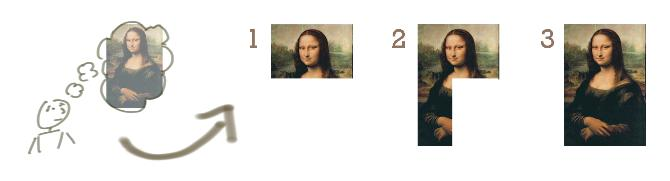
\includegraphics[width=0.8\textwidth]{Ilustraciones/metodologia/patton-incrementing-mona-lisa.jpg}
        \caption{Dibujo incremental de la Mona Lisa por Jeff Patton~\cite{monalisajp}}\label{fig:mona_iterativa}
    \end{figure}

    \item Por otro lado, el \textbf{método iterativo} se utiliza para construir funcionalidades gradualmente. Se desarrolla por entregas, incorporando en cada entrega una nueva funcionalidad. Para ello se debe establecer con bastante rigurosidad los resultados esperados. Si utilizamos nuevamente como referencia el ejemplo del dibujo, se construye poco a poco cada parte de la escena hasta completar la obra \figref{fig:mona_incremental}.
    
    \begin{figure}[H]
        \centering
        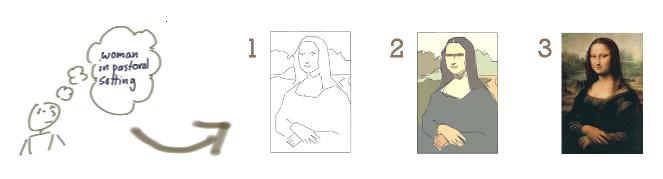
\includegraphics[width=0.8\textwidth]{Ilustraciones/metodologia/patton-iterating-mona-lisa.jpg}
        \caption{Dibujo iterativo de la Mona Lisa por Jeff Patton~\cite{monalisajp}}\label{fig:mona_incremental}
    \end{figure}
\end{itemize}

Si fusionamos los dos métodos obtenemos la \textbf{metodología iterativa e incremental}, la cual nos permite la construcción de software por entregas funcionales donde se implementarán y mejorarán funcionalidades simultáneamente. Continuando con el ejemplo del dibujo, comenzamos por elaborar un boceto y completar poco a poco las partes más importantes, tomando sugerencias del cliente para matizar en los detalles \figref{fig:mona_iterativa_incremental}.

\begin{figure}[H]
    \centering
    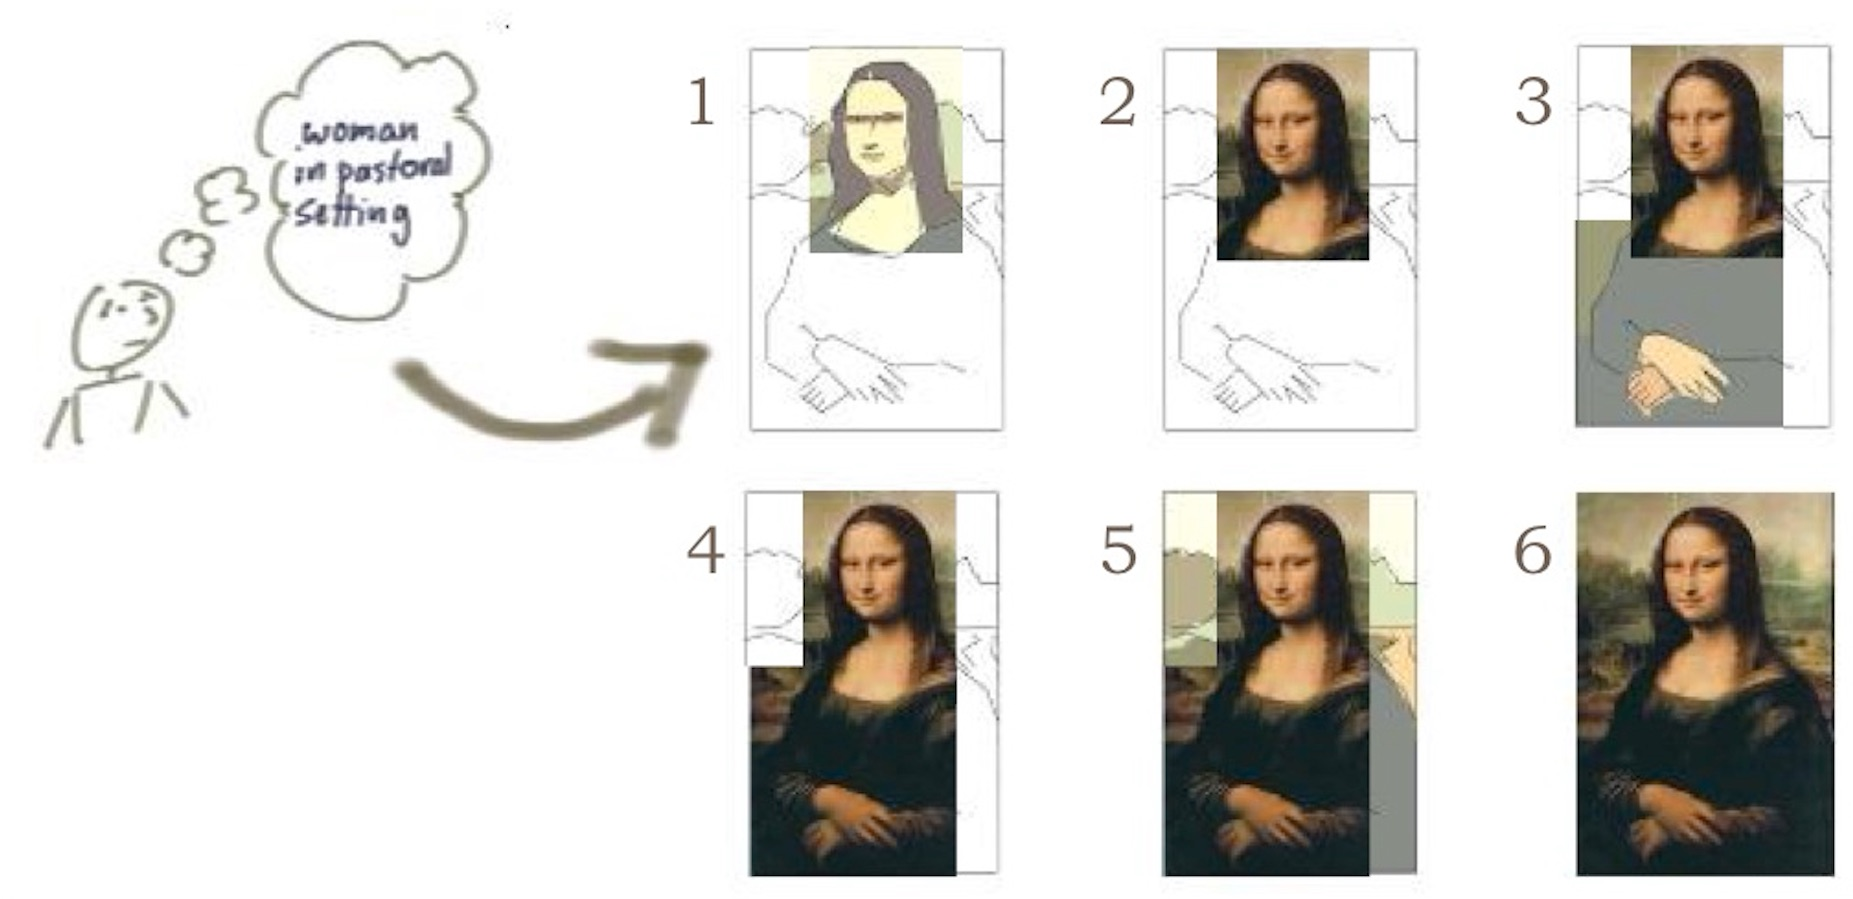
\includegraphics[width=0.8\textwidth]{Ilustraciones/metodologia/iterative-incremental-mona-lisa.jpeg}
    \caption{Dibujo incremental e iterativo de la Mona Lisa por Steven Thomas~\cite{monalisast}}\label{fig:mona_iterativa_incremental}
\end{figure}

Una vez definidos los conceptos que conforman la metodología iterativa e incremental, podemos elaborar el proceso de desarrollo. Este debe incluir las principales \textbf{fases de desarrollo software}; análisis, diseño, desarrollo, pruebas y entrega. Llamaremos \textbf{incremento} a cada repetición del proceso, que implica la implementación o mejora de una funcionalidad. Una vez finalizado el incremento, se entregará al usuario y se decidirá si es necesaria una nueva iteración \figref{fig:flujo_it_inc}.

\begin{figure}[H]
    \centering
    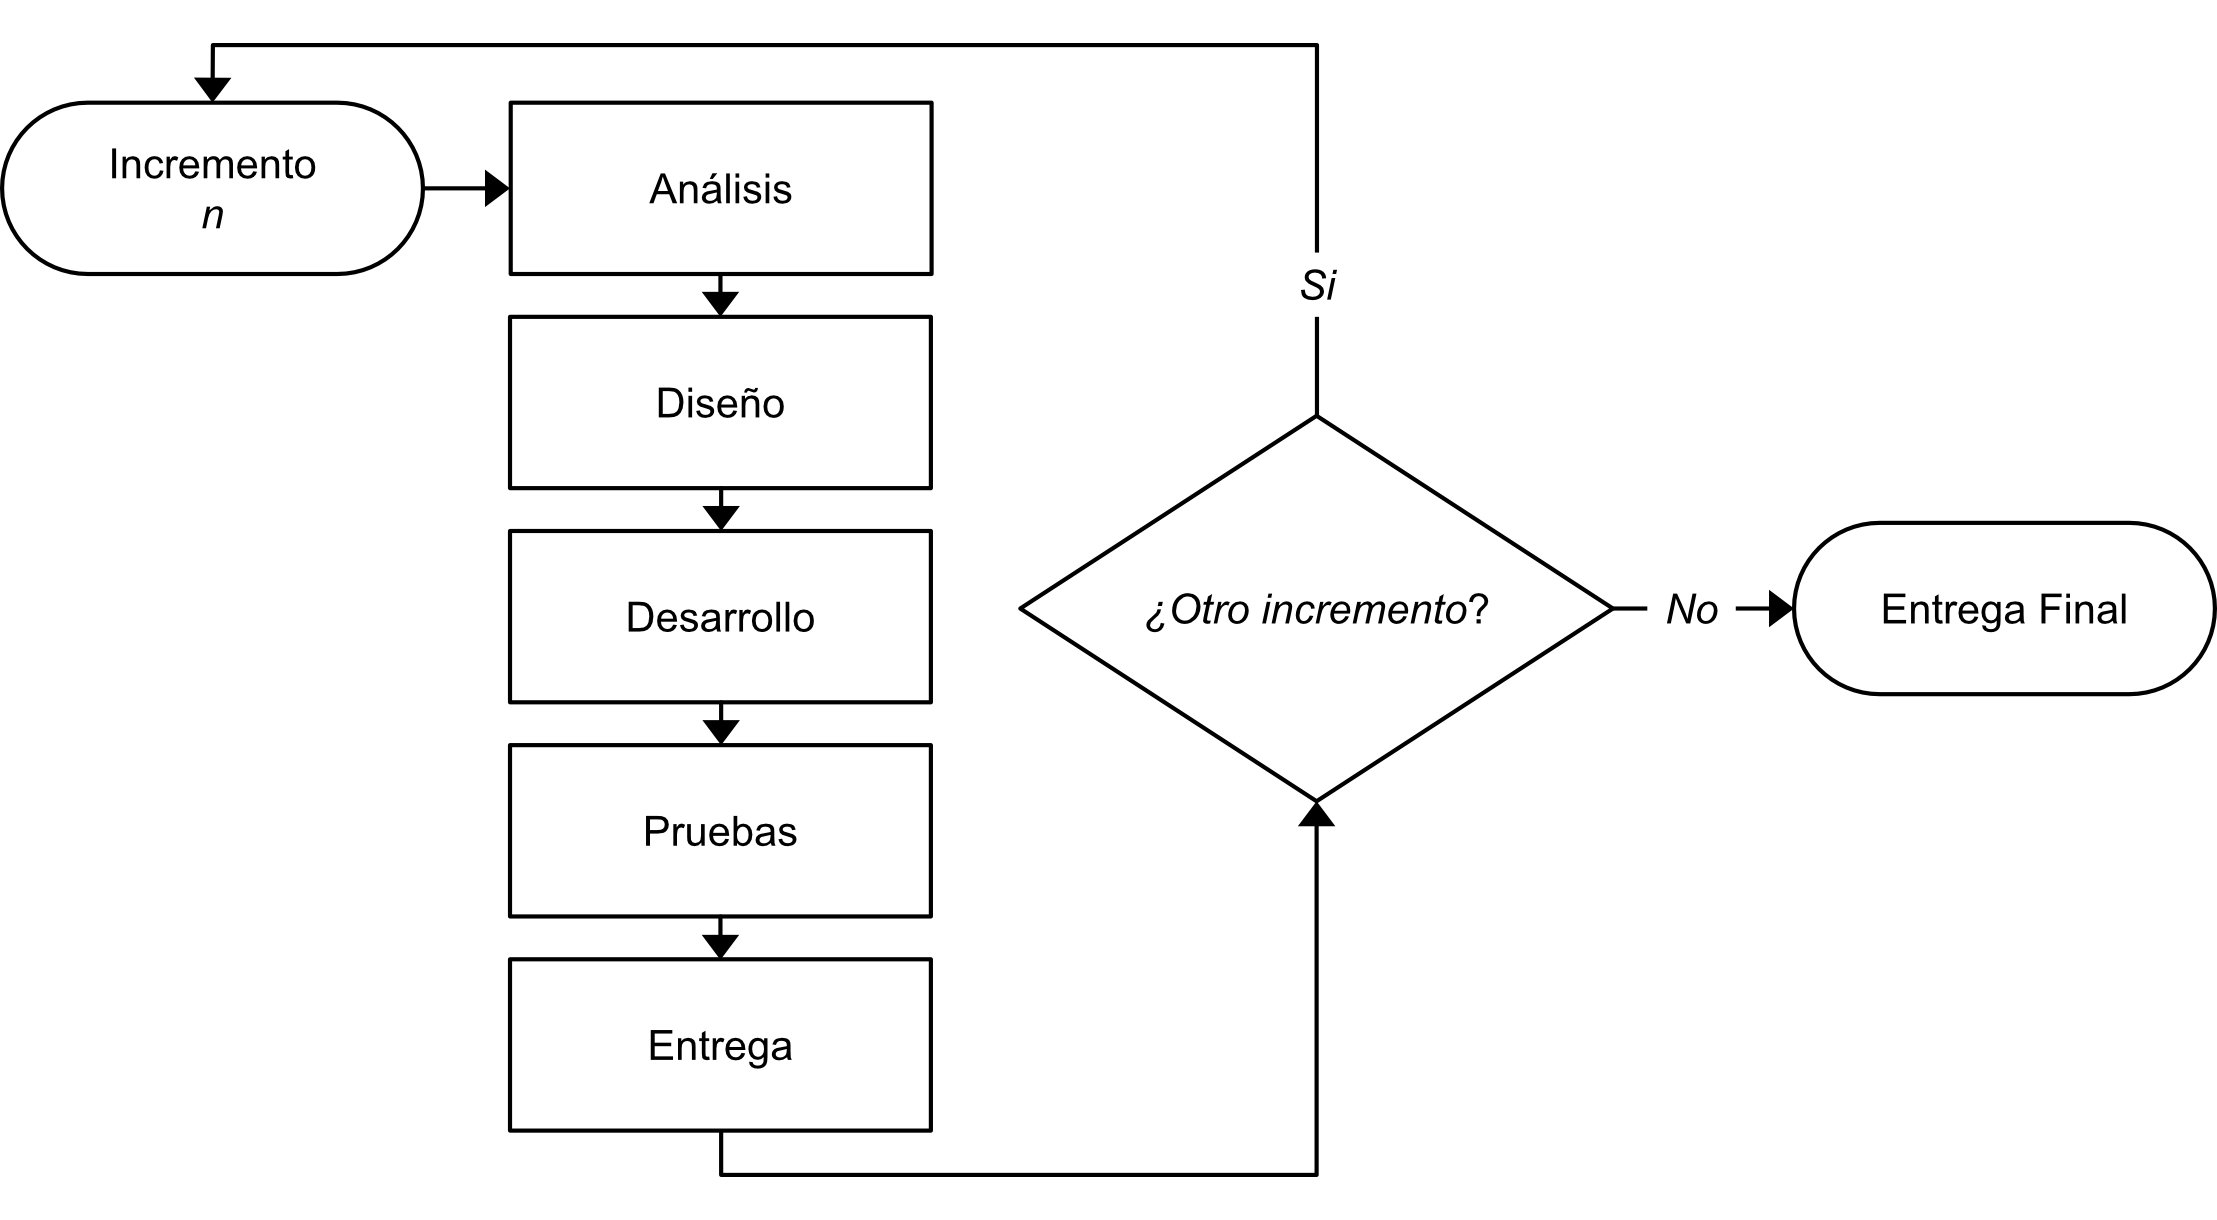
\includegraphics[width=0.8\textwidth]{Ilustraciones/metodologia/flujo_it_inc.jpg}
    \caption{Proceso de desarrollo de la metodología iterativa e incremental}\label{fig:flujo_it_inc}
\end{figure}

\section{Planificación}

El proyecto se desarrolló en tres fases: preproducción, desarrollo y postproducción. Cada fase contiene una serie de tareas a realizar, con una estimación en horas para cada fase \tabref{tab:fases_tareas}.

\begin{table}[H]
    \caption{Fases, estimación y tareas.}\label{tab:fases_tareas}
    \scriptsize
    \centering
    \begin{tabular}{lllp{0.45\textwidth}}
        \hline

        \textbf{Fase} & \textbf{Estimación} & \textbf{Tarea} & \textbf{Descripción} \\ \hline
        
        \multirow{2}{*}{Preproducción} 
        & 12h & 1.1 & Investigación de estado del arte. \\ 
        & 4h & 1.2 & Selección de tecnologías y herramientas. \\ \hline
        
        \multirow{6}{*}{Desarrollo} 
        & 50h & 2.1 & Configuración del proyecto, implementación de estructura básica de la web, autenticación y perfil de usuario. \\ 
        & 50h & 2.2 & Desarrollo de algoritmo de cálculo de acordes. \\ 
        & 50h & 2.3 & Implementación de páginas para la visualización y creación de publicaciones. \\ 
        & 36h & 2.4 & Desarrollo de biblioteca de publicaciones. \\ 
        & 24h & 2.5 & Implementación de componentes sociales. \\ 
        & 24h & 2.6 & Desarrollo de páginas informativas. \\ \hline
        
        \multirow{2}{*}{Postproducción} 
        & 46h & 3.1 & Redacción de memoria. \\ 
        & 4h & 3.2 & Elaboración de presentación. \\ \hline
        
    \end{tabular}
\end{table}

Además, durante la fase de \textbf{desarrollo} se aplicó la \textbf{metodología iterativa e icremental}, siendo cada tarea equivalente a un incremento \tabref{tab:incrementos}.

\begin{table}[H]
    \centering
    \scriptsize
    \caption{Fase de desarrollo; incrementos y descripción.}\label{tab:incrementos}
    \begin{tabular}{cp{0.6\textwidth}}
        \hline
        \textbf{Incremento} & \textbf{Descripción} \\ \hline
        1 & Configuración del proyecto, implementación de estructura básica de la web, autenticación y perfil de usuario. \\ 
        2 & Desarrollo de algoritmo de cálculo de acordes. \\
        3 & Implementación de páginas para la visualización y creación de publicaciones. \\
        4 & Desarrollo de biblioteca de publicaciones. \\
        5 & Implementación de componentes sociales. \\ 
        6 & Desarrollo de páginas informativas. \\ \hline
    \end{tabular}
\end{table}

Finalmente, durante la ejecución de cada incremento se siguió una variación del flujo de desarrollo mencionado anteriormente, sustituyendo al entrega por el despliegue del incremento, y añadiendo las fases de preproducción y postproducción como actividades de inicio y final respectivamente. \figref{fig:flujo_met}.

\begin{figure}[H]
    \centering
    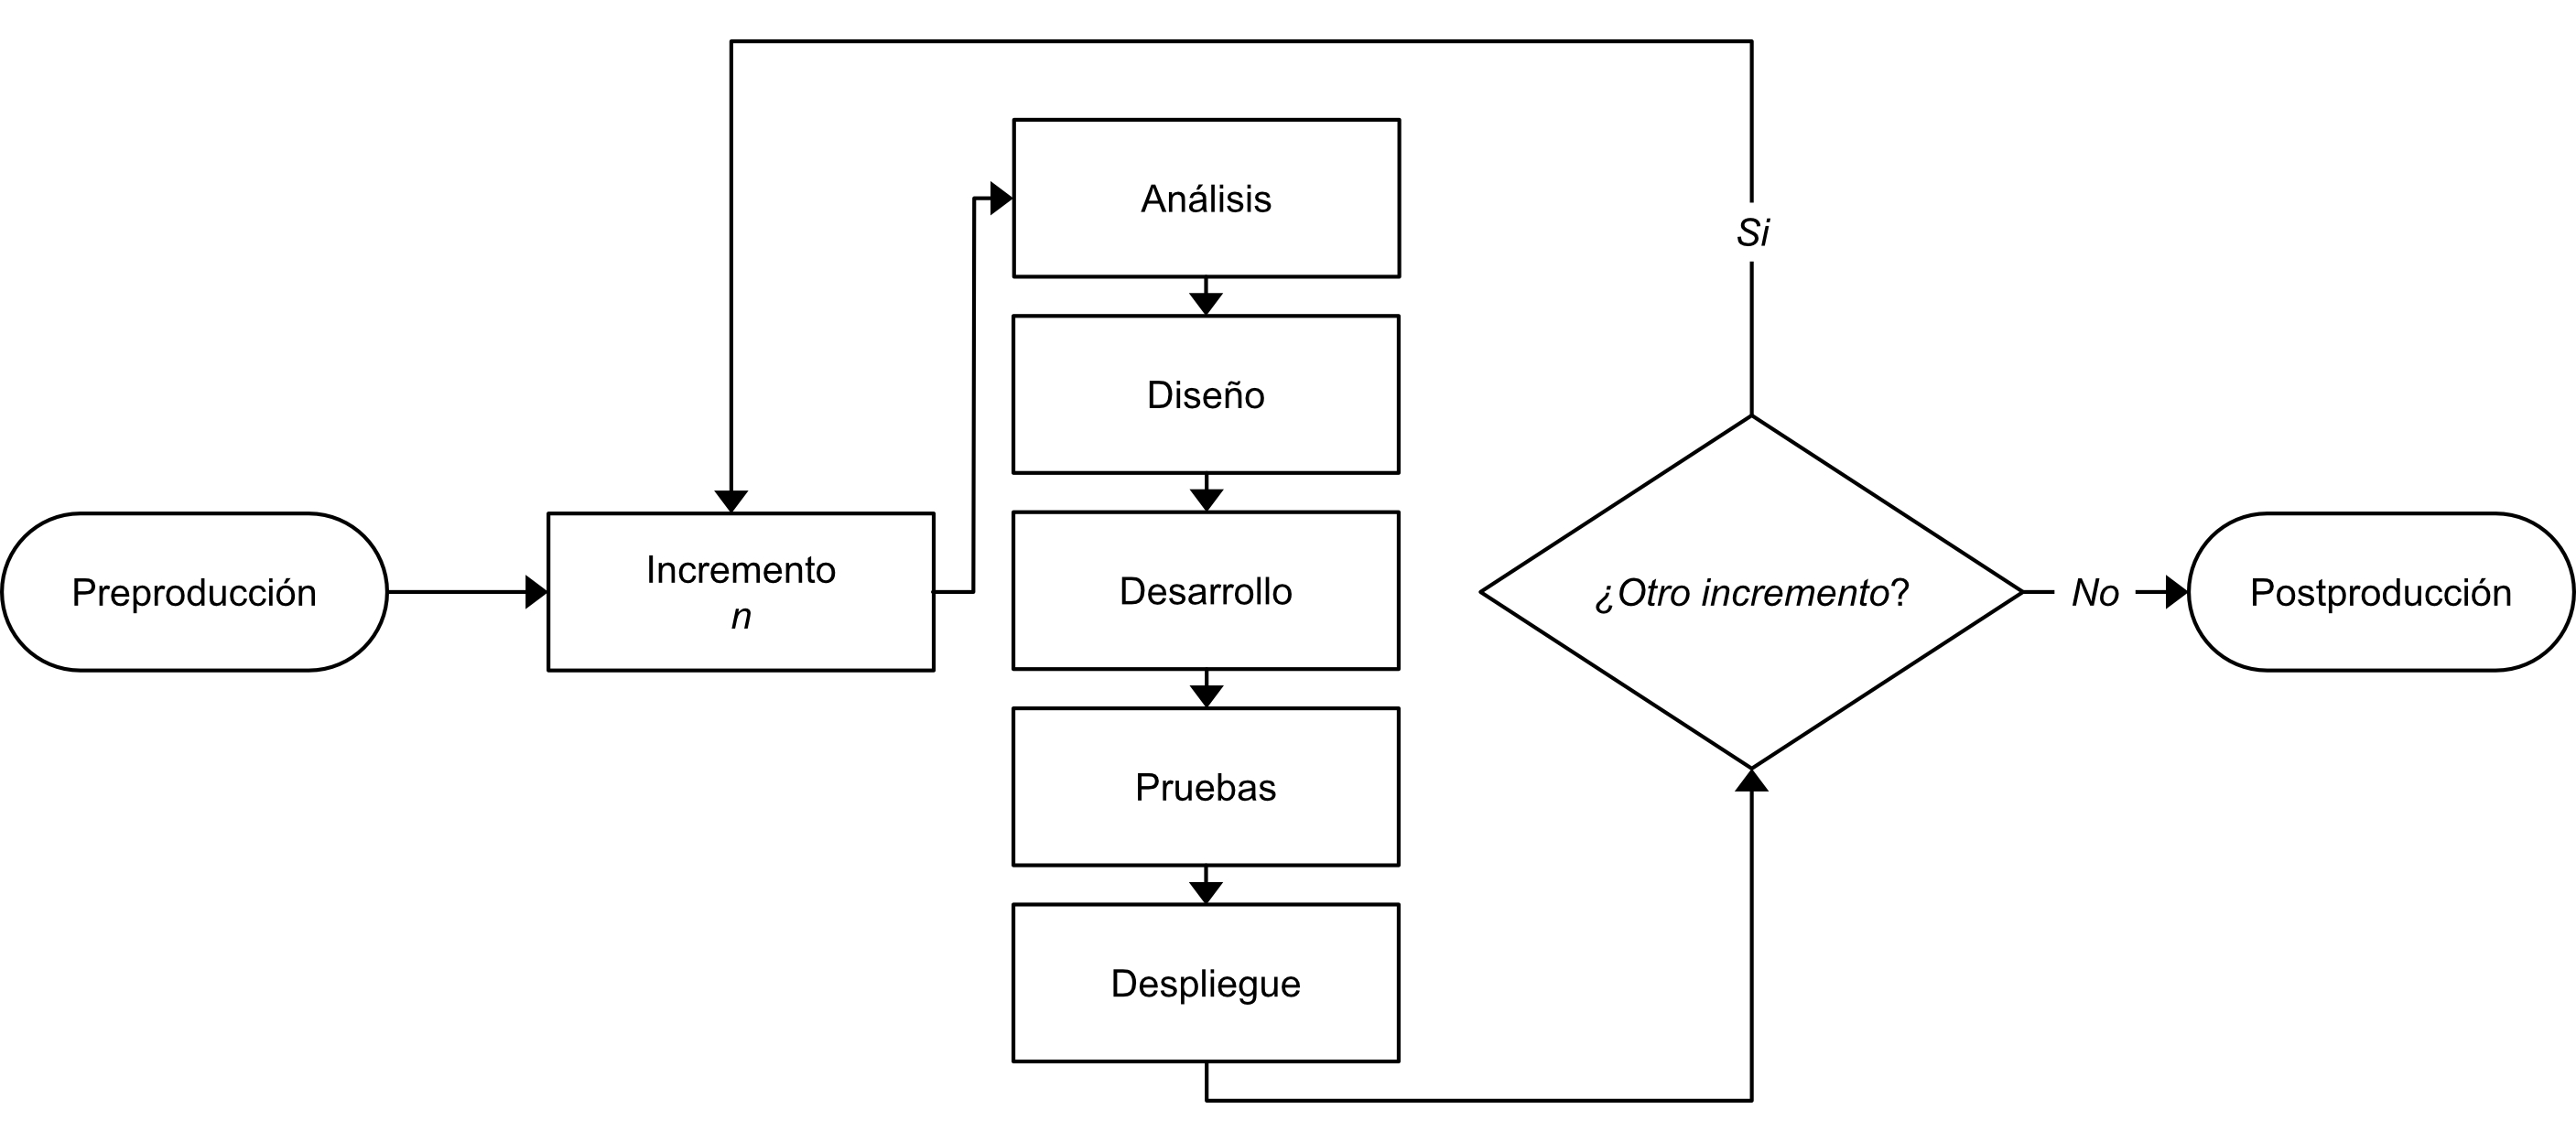
\includegraphics[width=1\textwidth]{Ilustraciones/metodologia/flujo_met.jpg}
    \caption{Proceso de desarrollo adaptado al proyecto}
    \label{fig:flujo_met}
\end{figure}

\chapter{Estado del Arte}
Este capítulo abarca aspectos como los fundamentos musicales necesarios para el desarrollo del proyecto, el estado actual, análisis de competencia y alcance del proyecto.

\section{Fundamentos musicales}

Para el desarrollo de este proyecto es imprescindible familiarizarse con ciertos aspectos fundamentales de la música. A continuación se describen los conceptos básicos sobre: musicología, instrumentos de cuerda pulsada y música digital.

\subsection{Conceptos básicos}
\label{c:fundamentos_musicales}

%----------------------------------------------------------------------------
% NOTACIÓN MUSICAL
%----------------------------------------------------------------------------
\subsubsection{Notación musical}
La \textbf{\gls{notación musical}}~\cite{wikipedia_notacion_musical} es el sistema de escritura que se utiliza con el fin de representar las notas musicales que conforman una canción. Estas pueden ser gráficas o alfabeticas, siendo las mas populares la \textbf{notación en pentagrama} \figref{fig:pentagrama}, la \textbf{\gls{notación latina}} y la \textbf{\gls{notación anglosajona}} \tabref{tab:equivalencia_notacion_ang_lat}.

\begin{figure}[H]
    \scriptsize
    %\centering
    % --- Figura a la izquierda ---
    \begin{minipage}[t]{0.48\textwidth}
        \vspace{0pt} % fuerza la alineación superior
        \centering
        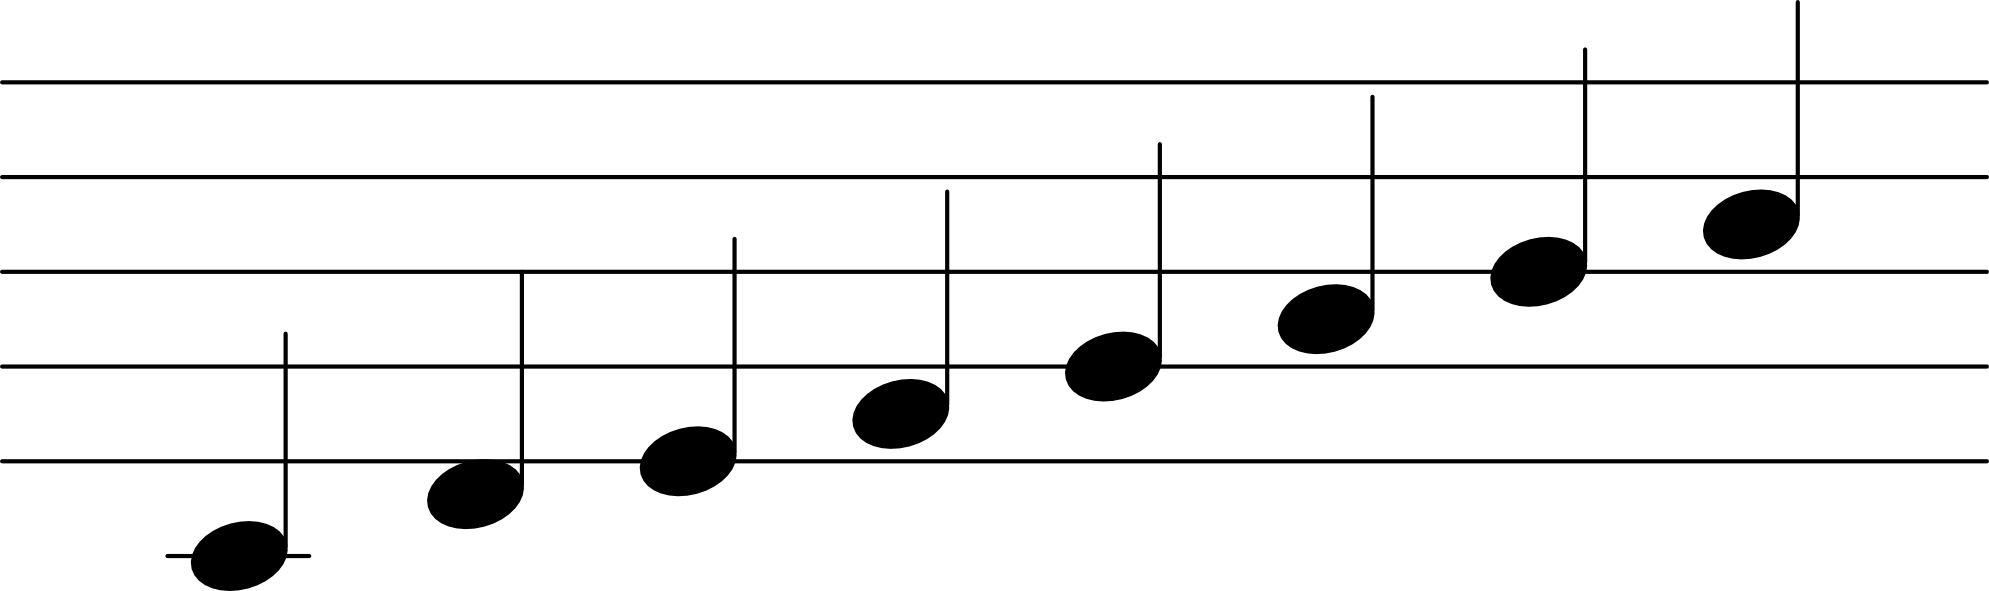
\includegraphics[width=\textwidth]{Ilustraciones/estado/pentagrama.jpg}
        \caption{Notación en pentagrama}\label{fig:pentagrama}
    \end{minipage}
    \hfill
    % --- Tabla a la derecha ---
    \begin{minipage}[t]{0.48\textwidth}
        % fuerza la alineación superior
        \vspace{23pt} 
        \centering
        \begin{tabular}{l c c c c c c c}
            \hline
            \textbf{Notación} & \multicolumn{7}{c}{\textbf{Notas}} \\
            \hline
            Latina & $Do$ & $Re$ & $Mi$ & $Fa$ & $Sol$ & $La$ & $Si$ \\
            Anglosajona & $C$ & $D$ & $E$ & $F$ & $G$ & $A$ & $B$ \\
            \hline
        \end{tabular}
        \captionof{table}{Notación latina y anglosajona}\label{tab:equivalencia_notacion_ang_lat}
    \end{minipage}
\end{figure}

\subsubsection{Notas musicales}
En teoría musical se identifican 7 notas naturales \textit{(e.g. teclas blancas del piano)}, entre las cuales se encuentran 5 notas llamadas \textbf{alteraciones} \textit{(e.g. teclas negras del piano)}. Distinguimos dos tipos de:

\begin{itemize}
    \item \textbf{Sostenido}, representado generalmente con el simbolo $\sharp$, se refiere a la nota contigua aguda \emph{(e.g. en el piano Do$\sharp$ es la tecla negra a la derecha de Do)}.
    
    \item \textbf{Bemol}, representado generalmente con el simbolo $\flat$, se refiere la la nota contigua grave \emph{(e.g. en el piano Re$\flat$ es la tecla negra a la izquierda de Re)}.
\end{itemize}

De este modo, podemos afirmar la existencia de 12 notas \figref{fig:piano_notas}.

\begin{figure}[H]
    \centering
    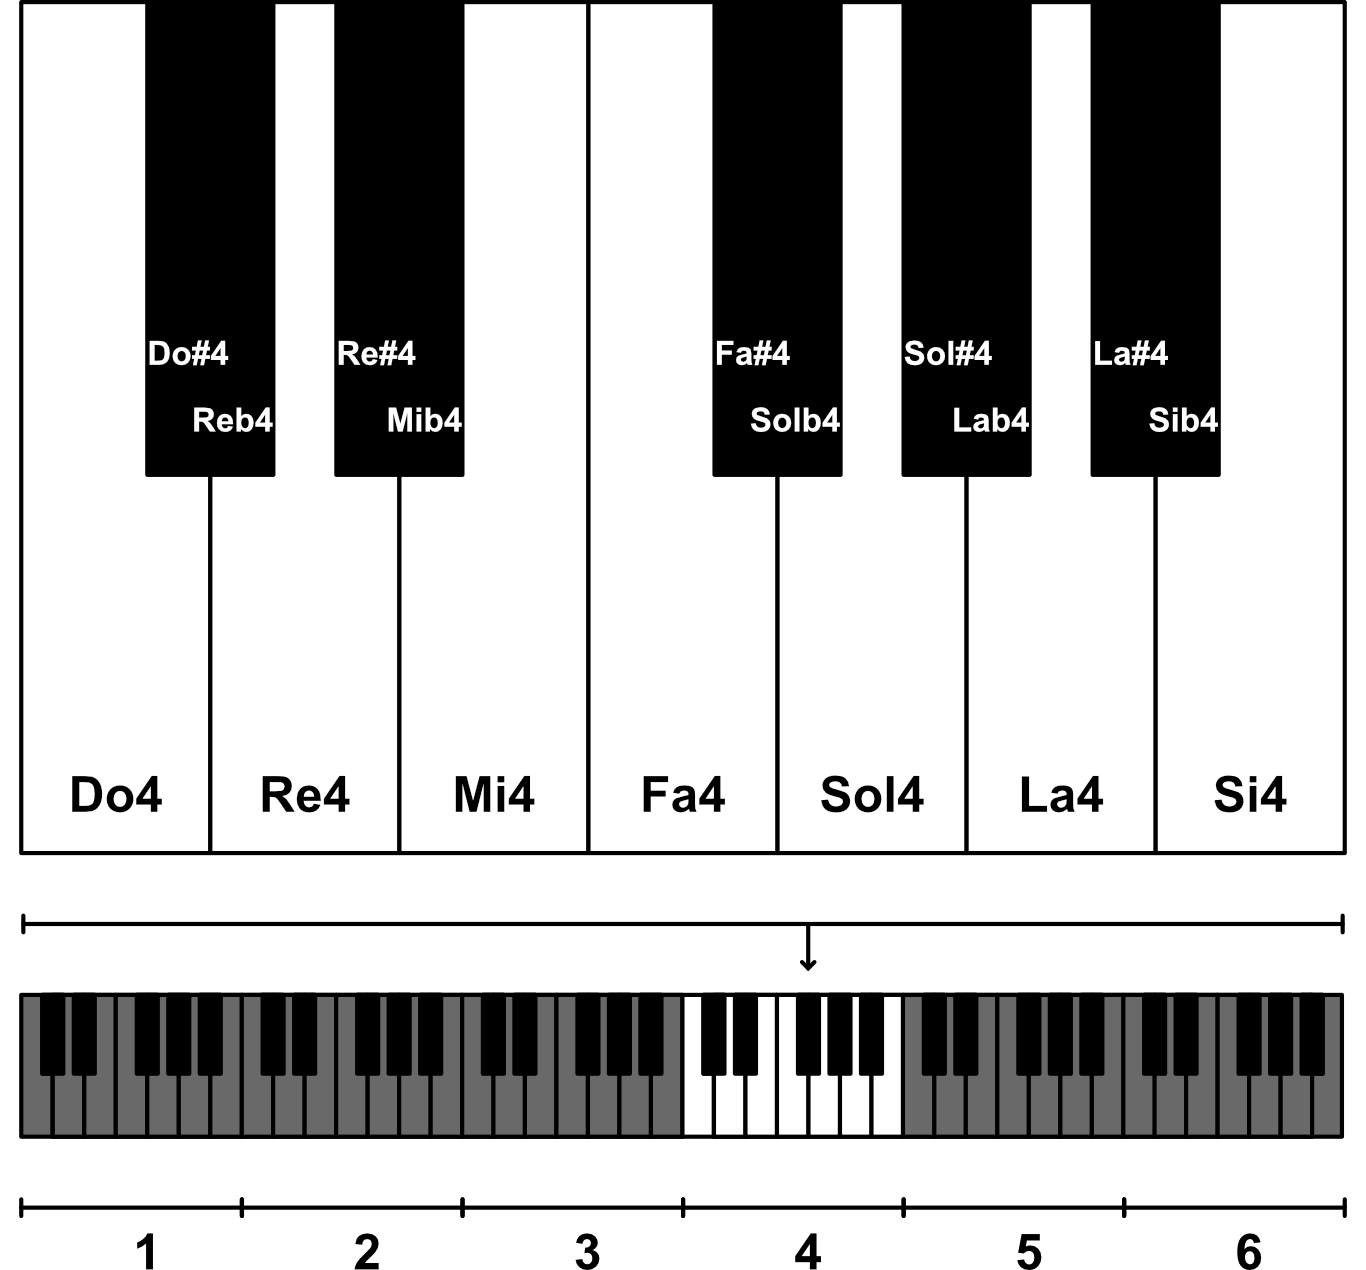
\includegraphics[width=0.5\textwidth]{Ilustraciones/estado/piano_cromatica.jpg}
    \caption{Notas en un piano}\label{fig:piano_notas}
\end{figure}

La distribución de las alteraciones no es arbitraria y debemos introducir el concepto de distancia entre notas:

\begin{itemize}
    \item El \textbf{\gls{semitono}}, que es la distancia mínima entre dos notas contiguas \emph{(e.g. la distancia entre dos teclas adyacentes del piano)}.

    \item El \textbf{\gls{tono}}, equivalente a dos semitonos \emph{(e.g. la distancia entre dos teclas blancas que tienen una tecla negra entre ellas)}.
\end{itemize}

Una alteración se ubicará entre dos notas naturales con una distancia de 1 tono \textit{(i.e. dos semitonos)} \tabref{tab:notas}.

\begin{table}[H]
        \centering
        \scriptsize
        \caption{Notas naturales, alteraciones y semitonos}\label{tab:notas}
        \begin{tabular}{l c c c c c c c c c c c c c}
        \hline
        \textbf{Naturales} & $Do$ & & $Re$ & & $Mi$ & $Fa$ & & $Sol$ & & $La$ & & $Si$ \\
        \textbf{Alteraciones} & & $Do\sharp$ & & $Re\sharp$ & & & $Fa\sharp$ & & $Sol\sharp$ & & $La\sharp$ & \\
        \textbf{Semitono} & 0 & 1 & 2 & 3 & 4 & 5 & 6 & 7 & 8 & 9 & 10 & 11 \\
        
        \hline
    \end{tabular}
\end{table}

%----------------------------------------------------------------------------
% ESCALA MUSICAL
%----------------------------------------------------------------------------
\subsubsection{Escala musical}
Dado un conjunto de notas, su orden en una secuencia se conoce como \textbf{\gls{escala musical}}~\cite{wikipedia_escala_musical}, caracterizada por:

\begin{itemize}
    \item Poseer un orden en sentido ascendente (de grave a agudo) o descendente (de agudo a grave).
    \item Definir una nota inicial o \textbf{tónica}.
    \item Seguir un patrón de distancias.
\end{itemize}

Además, podemos distinguir el concepto de \textbf{octava} que es el intervalo de notas entre dos iguales \emph{e.g. de Do a Do'}. Este invervalo puede variar según la escala:

\begin{itemize}
    \item La \textbf{escala diatónica}, conformada por 7 notas siguiendo el patrón: tono, tono, semitono, tono, tono, tono y semitono. Cada nota posee un \textbf{grado} que actúa como índice y indicador de la distancia a la tónica. Cada grado posee también un nombre propio \tabref{tab:escala_diatonica}.

    \begin{table}[H]
        \centering
        \scriptsize
        \caption{Escalas diatónicas y octavas con tónicas en $Do$ y en $Re$}\label{tab:escala_diatonica}
        \begin{tabular}{l c c c c c c c c}
            \hline
            & \textbf{I} & \textbf{II} & \textbf{III} & \textbf{IV} & \textbf{V} & \textbf{VI} & \textbf{VII} & \textbf{VIII} \\
            & {\tiny Tónica} & {\tiny Supertónica} & {\tiny Mediante} & {\tiny Subdominante} & {\tiny Dominante} & {\tiny Supermediante} & {\tiny Sensible} & {\tiny Octava}  \\
            \hline
            Escala & $Do$ & $Re$ & $Mi$ & $Fa$ & $Sol$ & $La$ & $Si$ &  \\
            Octava & $Do$ & $Re$ & $Mi$ & $Fa$ & $Sol$ & $La$ & $Si$ & $Do'$  \\
            \hline
            Escala & $Re$ & $Mi$ & $Fa\sharp$ & $Sol$ & $La$ & $Si$ & $Do$ &  \\
            Octava & $Re$ & $Mi$ & $Fa\sharp$ & $Sol$ & $La$ & $Si$ & $Do$ & $Re'$  \\
            \hline
        \end{tabular}
    \end{table}
    
    \item La \textbf{escala cromática}, conformada por 12 notas siguiendo un patrón de 12 semitonos \tabref{tab:escala_cromatica}
    
    \begin{table}[H]
        \centering
        \caption{Escalas cromáticas y octavas con tónicas en $Do$ y en $Re$}\label{tab:escala_cromatica}
        \scriptsize
        \begin{tabular}{l c c c c c c c c c c c c c}
            \hline
            Escala & $Do$ & $Do\sharp$ & $Re$ & $Re\sharp$ & $Mi$ & $Fa$ & $Fa\sharp$ & $Sol$ & $Sol\sharp$ & $La$ & $La\sharp$ & $Si$ \\
            Octava & $Do$ & $Do\sharp$ & $Re$ & $Re\sharp$ & $Mi$ & $Fa$ &
            $Fa\sharp$ & $Sol$ & $Sol\sharp$ & $La$ & $La\sharp$ & $Si$ & $Do'$ \\
            \hline
            Escala & $Re$ & $Re\sharp$ & $Mi$ & $Fa$ & $Fa\sharp$ & $Sol$ & $Sol\sharp$ & $La$ & $La\sharp$ & $Si$ & $Do$ & $Do\sharp$ \\
            Octava & $Re$ & $Re\sharp$ & $Mi$ & $Fa$ & $Fa\sharp$ & $Sol$ & $Sol\sharp$ & $La$ & $La\sharp$ & $Si$ & $Do$ & $Do\sharp$ & $Re'$ \\
            \hline
        \end{tabular}
    \end{table}
\end{itemize}

%----------------------------------------------------------------------------
% ACORDES
%----------------------------------------------------------------------------
\subsubsection{Acordes}
Un \textbf{\gls{acorde}}~\cite{wikipedia_acorde} es un conjunto de tres o más notas diferentes que conforman una unidad armónica. Entre los más populares encontramos las \textbf{tríadas} y \textbf{cuatríadas} (o \textbf{séptima}), construídos con tres y cuatro notas respectivamente. 

Para construir un acorde debemos seleccionar una \textbf{\gls{cualidad}} que indicará las distancias en semitonos de las notas \tabref{tab:acordes_cualidades}.

\begin{table}[H]
    \centering
    \caption{Modalidades de acordes}\label{tab:acordes_cualidades}
    \scriptsize
    \begin{tabular}{l c l}
        \hline
        \textbf{Cualidad} & \textbf{Símbolo} & \textbf{Semitonos} \\
        \hline
        Mayor & M & 0, 4, 7 \\
        Menor & m & 0, 3, 7 \\
        Aumentado & aug & 0, 4, 8 \\
        Disminuido & dim & 0, 3, 6 \\
        Séptima & 7 & 0, 4, 7, 10 \\
        Séptima mayor & M7 & 0, 4, 7, 11 \\
        Menor séptima & m7 & 0, 3, 7, 10 \\
        Menor séptima mayor & mM7 & 0, 3, 7, 11 \\
        \hline
    \end{tabular}
\end{table}

Por tanto, para tocar el acorde de $Do Mayor$ (también conocido como DoM o simplemente $Do$), establecemos como tónica la nota $Do$, y seleccionamos las notas correspondientes a las distancias en semitonos 0, 4, 7: es decir, $Do$, $Mi$ y $Sol$ \figref{fig:piano_acorde_doM}.

\begin{figure}[H]
    \centering
    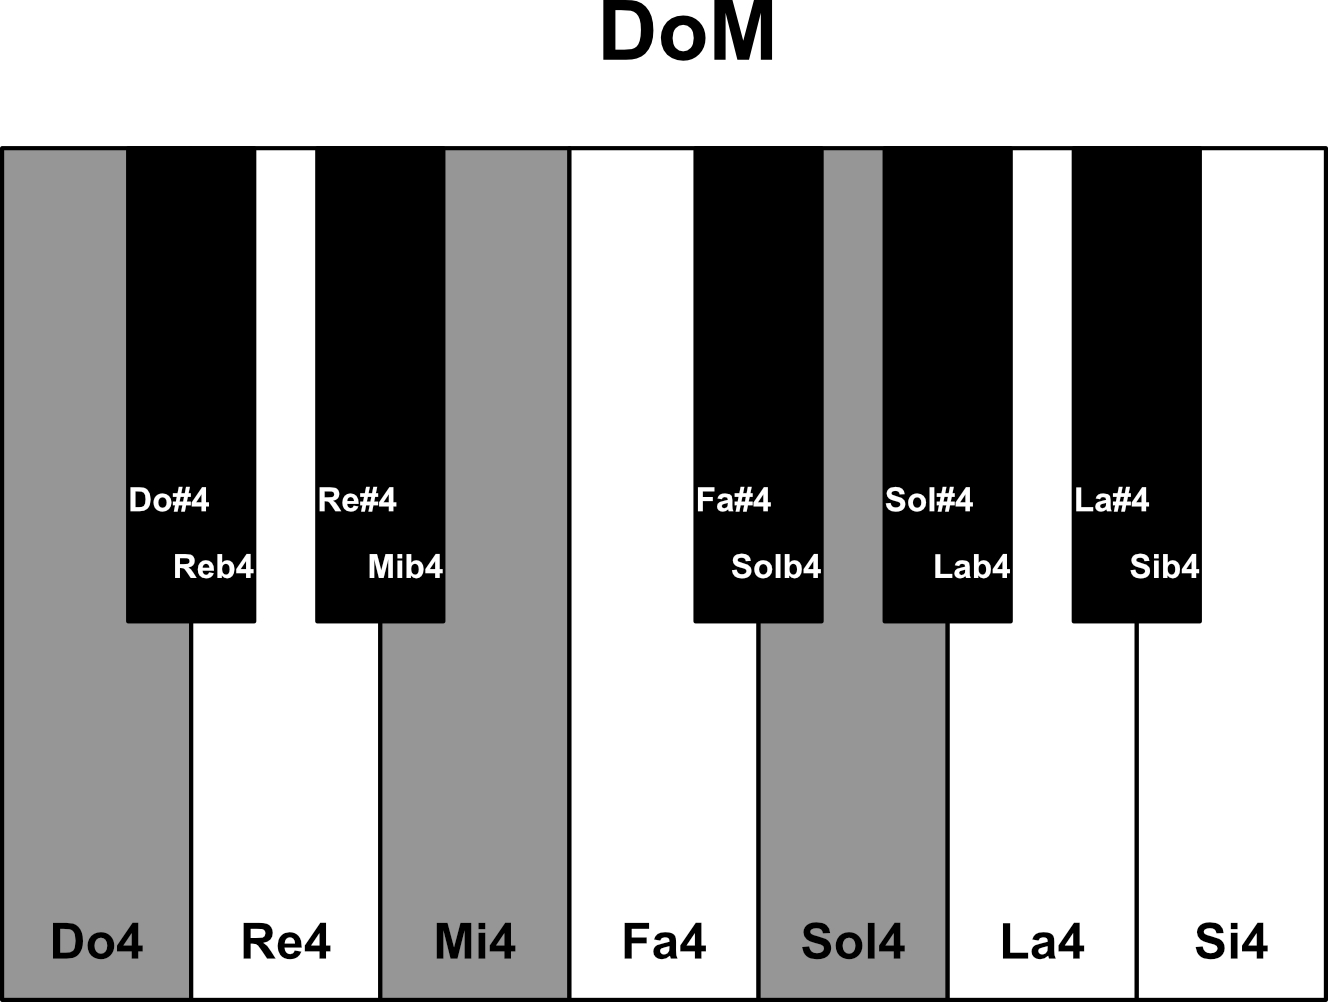
\includegraphics[width=0.5\textwidth]{Ilustraciones/estado/piano_doM.jpg}
    \caption{Acorde de $Do Mayor$ en piano}\label{fig:piano_acorde_doM}
\end{figure}

A una sucesión de acordes lo llamamos \textbf{\gls{progresión}}~\cite{wikipedia_progresion} \emph{(e.g. una progresión popular en el folclore canario es ReM, SolM y LaM)}.

Conocidos los conceptos de acorde y progresión, podemos introducir la \textbf{\gls{transposición}}. Dado un \textbf{acorde raiz}, podemos mover la tónica un semitono a la izquierda o a la derecha para obtener el acorde traspuesto. Si hablamos de una progresión, se realizará la operación anterior en todos los acordes que lo conforman \tabref{tab:transposicion_acordes_progresiones}.

\begin{table}[H]
    \centering
    \caption{Transposición un acorde y una progresión}\label{tab:transposicion_acordes_progresiones}
    \scriptsize
    \begin{tabular}{l l l}
        \hline
        \textbf{Transposición} & \textbf{Acorde} & \textbf{Progresión} \\
        \hline
        Raíz & $DoM$ & $DoM–FaM–SolM$ \\
        +1 & \textit{Do$\sharp$M} & \textit{Do$\sharp$M–Fa$\sharp$M–Sol$\sharp$M} \\
        +2 & \textit{ReM} & \textit{ReM–SolM–LaM} \\
        \hline
    \end{tabular}
\end{table}

%----------------------------------------------------------------------------
% TONALIDAD
%----------------------------------------------------------------------------
\subsubsection{Tonalidad}
La \textbf{tonalidad}~\cite{wikipedia_tonalidad} es un conjunto de notas que, relaciona una escala diatónica con acordes. De este modo podemos realizar asociaciones como:

\begin{itemize}
    \item \textbf{¿A qué tonalidad pertenece un acorde?} 
      El acorde de \textit{Re menor}, construido con las notas $Re$, $Mi$ y $Sol$, 
      pertenece a la tonalidad de \textit{DoM}, ya que todas sus notas forman parte de dicha tonalidad.
    \item \textbf{¿Que acordes pertenecen a una tonalidad?}
      Para la tonalidad de \textit{Do Mayor}, perteneceran solo los acordes cuyas notas se encuentre en su escala, como \textit{DoM}, \textit{Rem}\dots
\end{itemize}

Además, la tonalidad nos permite ordenar los acordes utilizando los grados de la escala diatónica \tabref{tab:ejemplos_tonalidades}, abriendo un gran abaníco de posibilidades como facilitar la creación de progresiones.

\begin{table}[H]
    \centering
    \caption{Acordes y notas en las tonalidades de $Do$ y $Re$ Mayor}\label{tab:ejemplos_tonalidades}
    \scriptsize
    \begin{tabular}{l c c c c c c c}
        \hline
        \multicolumn{8}{c}{\textbf{Tonalidad de Do Mayor}} \\
        \hline
        \multirow{2}{*}{\textbf{Acorde}} & \multicolumn{7}{c}{\textbf{Notas}} \\
         & \textit{Do} & \textit{Re} & \textit{Mi} & \textit{Fa} & \textit{Sol} & \textit{La} & \textit{Si} \\
        \hline
        
        % --- Tonalidad de Do mayor ---
        \textit{DoM (I)} & \ding{51} &  & \ding{51} &  & \ding{51} &  &  \\
        \textit{Rem (II)} &  & \ding{51} &  & \ding{51} &  & \ding{51} &  \\
        \textit{Mim (III)} &  &  & \ding{51} &  & \ding{51} &  & \ding{51} \\
        \textit{FaM (IV)} & \ding{51} &  &  & \ding{51} &  & \ding{51} &  \\
        \textit{SolM (V)} &  & \ding{51} &  &  & \ding{51} &  & \ding{51} \\
        \textit{Lam (VI)} & \ding{51} &  & \ding{51} &  &  & \ding{51} &  \\
        \textit{Sidim (VII)} &  & \ding{51} &  & \ding{51} &  &  & \ding{51} \\
        \hline
        \hline
        % --- Tonalidad de Re mayor ---
        \multicolumn{8}{c}{\textbf{Tonalidad de Re Mayor}} \\
        \hline
        \multirow{2}{*}{\textbf{Acorde}} & \multicolumn{7}{c}{\textbf{Notas}} \\
         & \textit{Re} & \textit{Mi} & \textit{Fa$\sharp$} & \textit{Sol} & \textit{La} & \textit{Si} & \textit{Do$\sharp$} \\
        \hline
        \textit{ReM (I)} & \ding{51} &  & \ding{51} &  & \ding{51} &  &  \\
        \textit{Mim (II)} &  & \ding{51} &  & \ding{51} &  & \ding{51} &  \\
        \textit{Fa$\sharp$m (III)} &  &  & \ding{51} &  & \ding{51} &  & \ding{51} \\
        \textit{SolM (IV)} & \ding{51} &  &  & \ding{51} &  & \ding{51} &  \\
        \textit{LaM (V)} &  & \ding{51} &  &  & \ding{51} &  & \ding{51} \\
        \textit{Sim (VI)} & \ding{51} &  & \ding{51} &  &  & \ding{51} &  \\
        \textit{Do$\sharp$dim (VII)} &  & \ding{51} &  & \ding{51} &  &  & \ding{51} \\
        \hline
    \end{tabular}
\end{table}




\subsection{Instrumentos de cuerda pulsada}
\label{c:fundamentos_cuerda}
Los \textbf{instrumentos de cuerda pulsada}~\cite{wikipedia_cuerdapulsada}, son aquellos que se tocan utilizando los dedos, las uñas o una púa. Podemos identificar dos elementos comunes:

\begin{itemize}
    \item Las \textbf{cuerdas}, normalmente nombradas con un índice comenzando por la derecha. Cada cuerda posee una \textbf{\gls{afinación}}, es decir, se le ha aplicado cierta tensión, de modo que seá capaz de reproducir una nota.
    \item Los \textbf{trastes}, unas tiras metálicas perpendiculares al mástil que, al igual que las cuerdas, reciben un nombre a modo de índice, comenzando desde arriba. Al presionar una cuerda sobre un traste se puede reproducir una nota más aguda a la afinada. Si tocamos la cuerda sin presionar ningún traste lo llamaremos \textbf{\gls{cuerda al aire}}.
\end{itemize}

La configuración de cuerdas y trastes \figref{fig:timple_partes} es equivalente a las teclas de un piano, es decir, si afinamos una cuerda en $Do$, los trastes bajo la misma serán equivalentes a las teclas de un piano comenzando en $Do$ \figref{fig:timple_notas_piano}

\begin{figure}[H]
    \centering
    \begin{subfigure}[t]{0.56\textwidth}
        \centering
        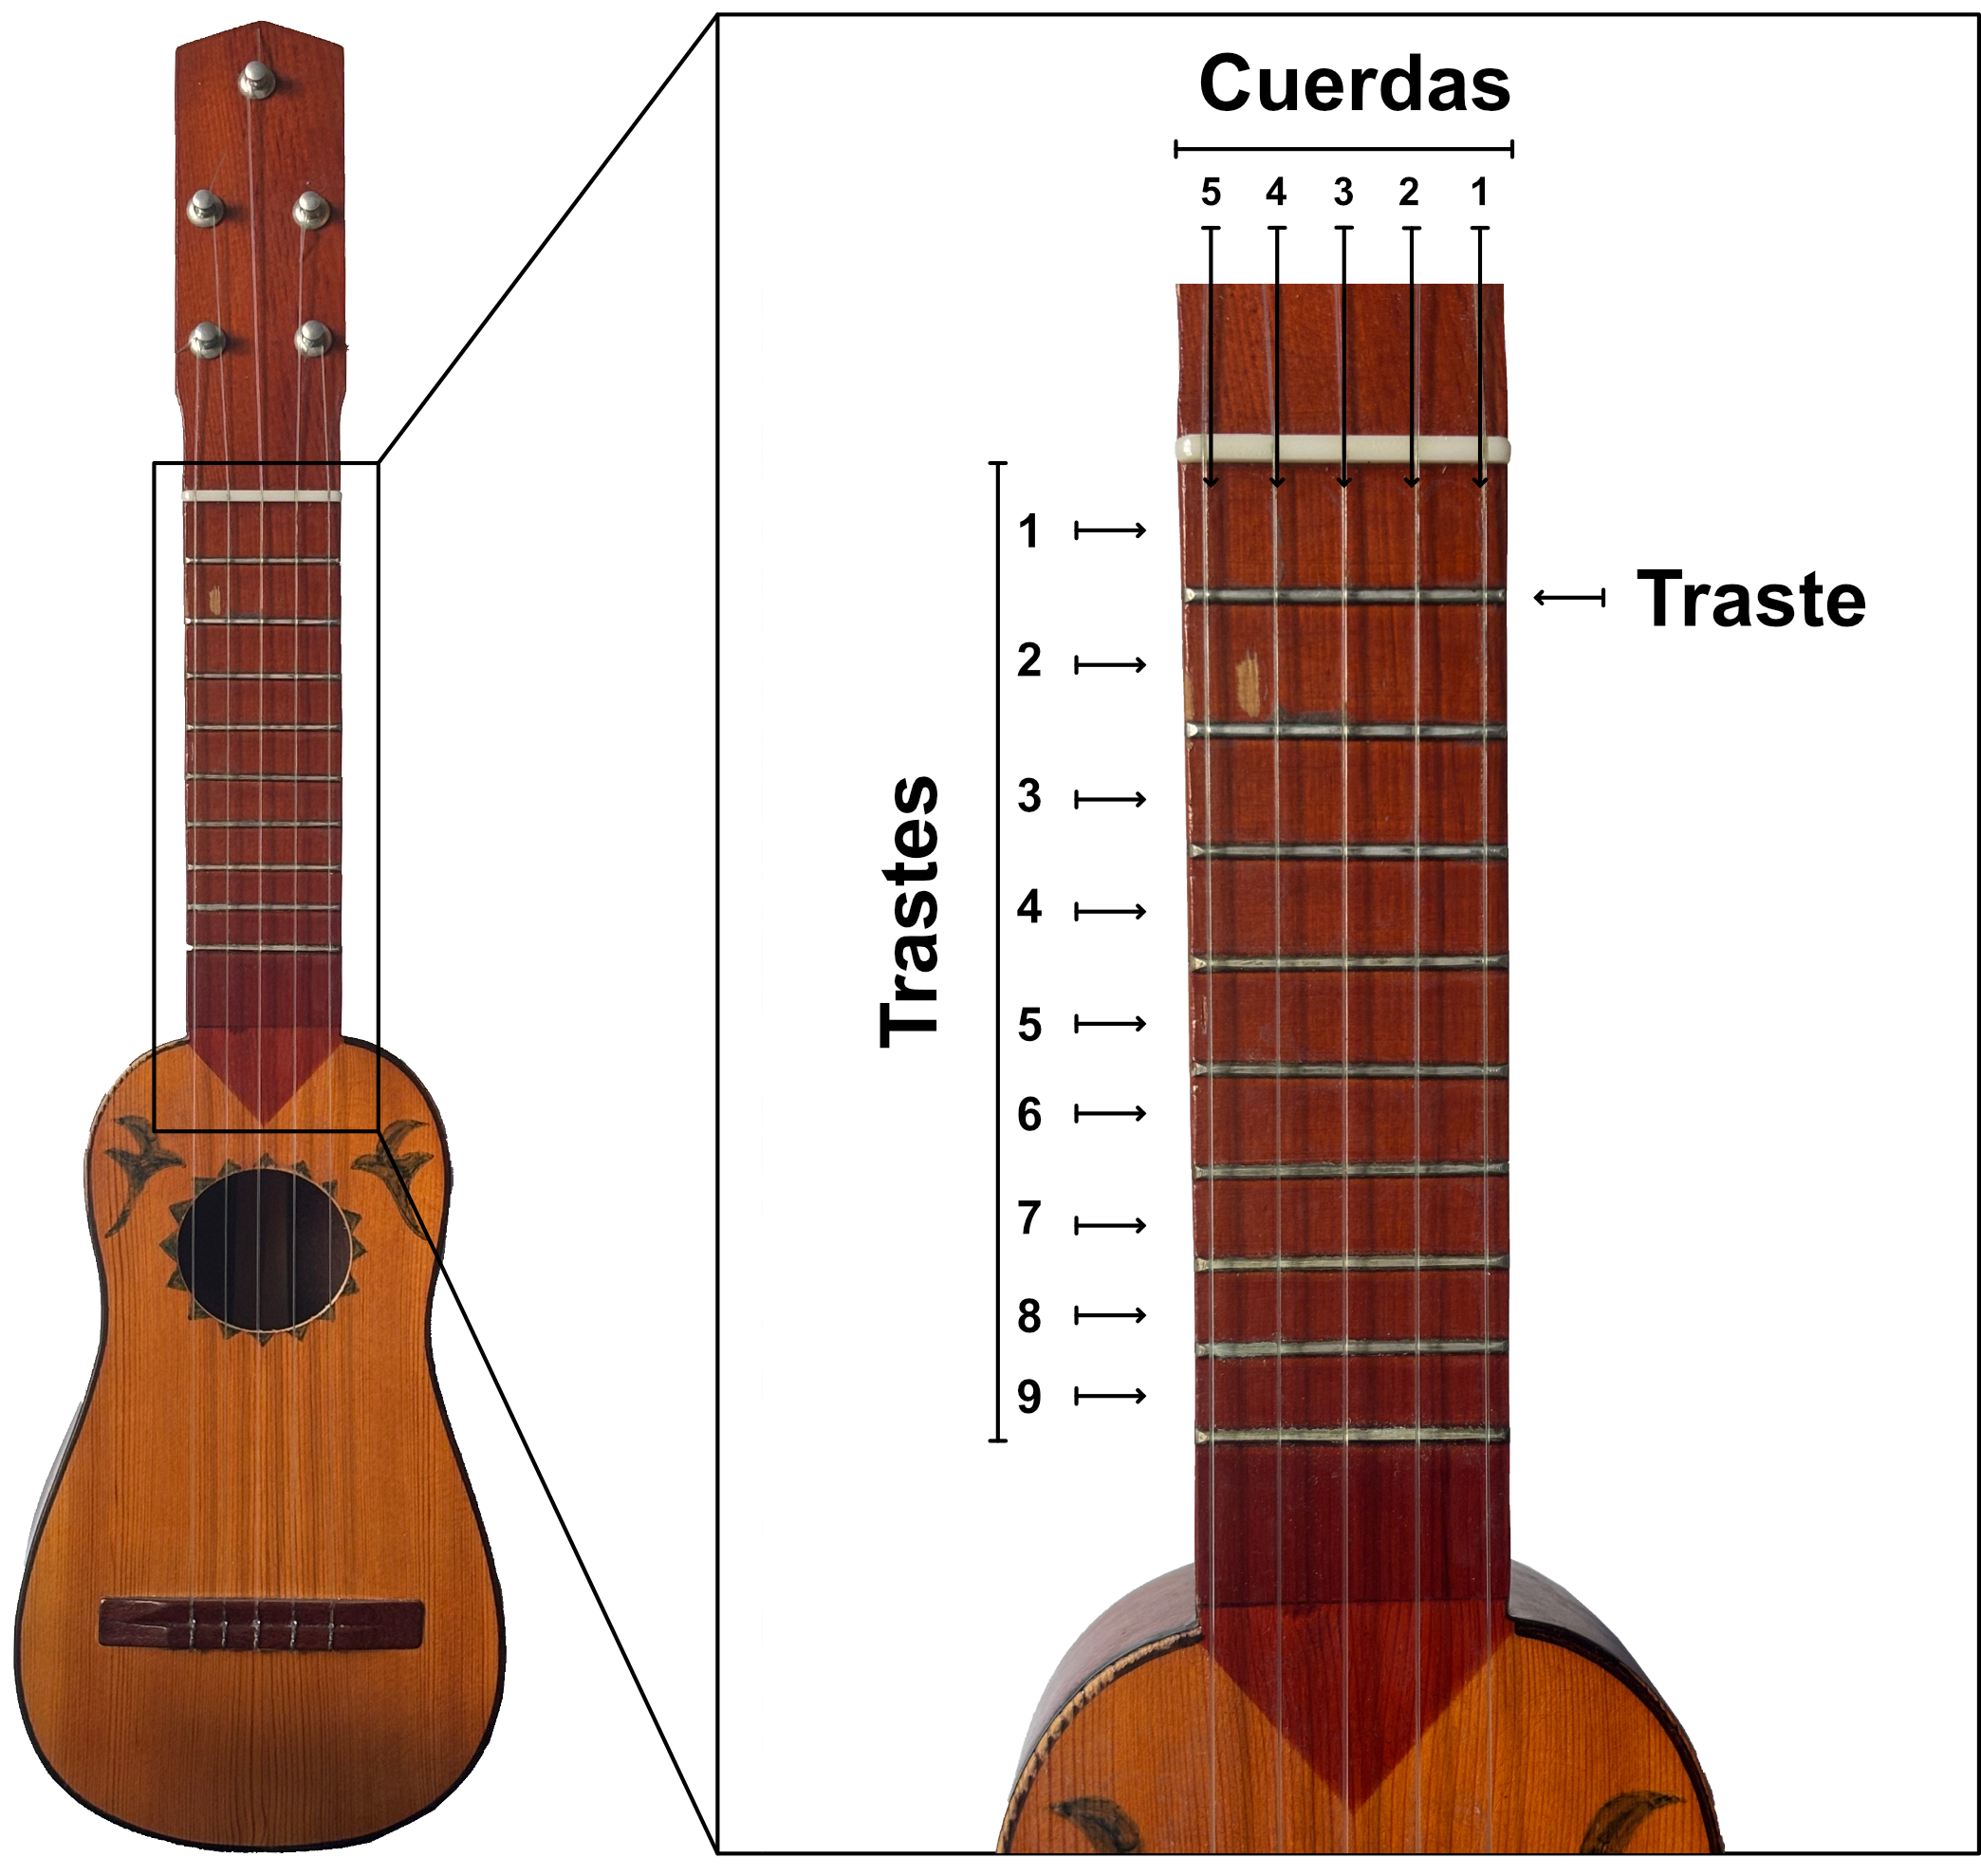
\includegraphics[width=\textwidth]{Ilustraciones/estado/timple_partes.jpg}
        \caption{Trastes y cuerdas en un timple}
        \label{fig:timple_partes}
    \end{subfigure}
    \hfill
    \begin{subfigure}[t]{0.40\textwidth}
        \centering
        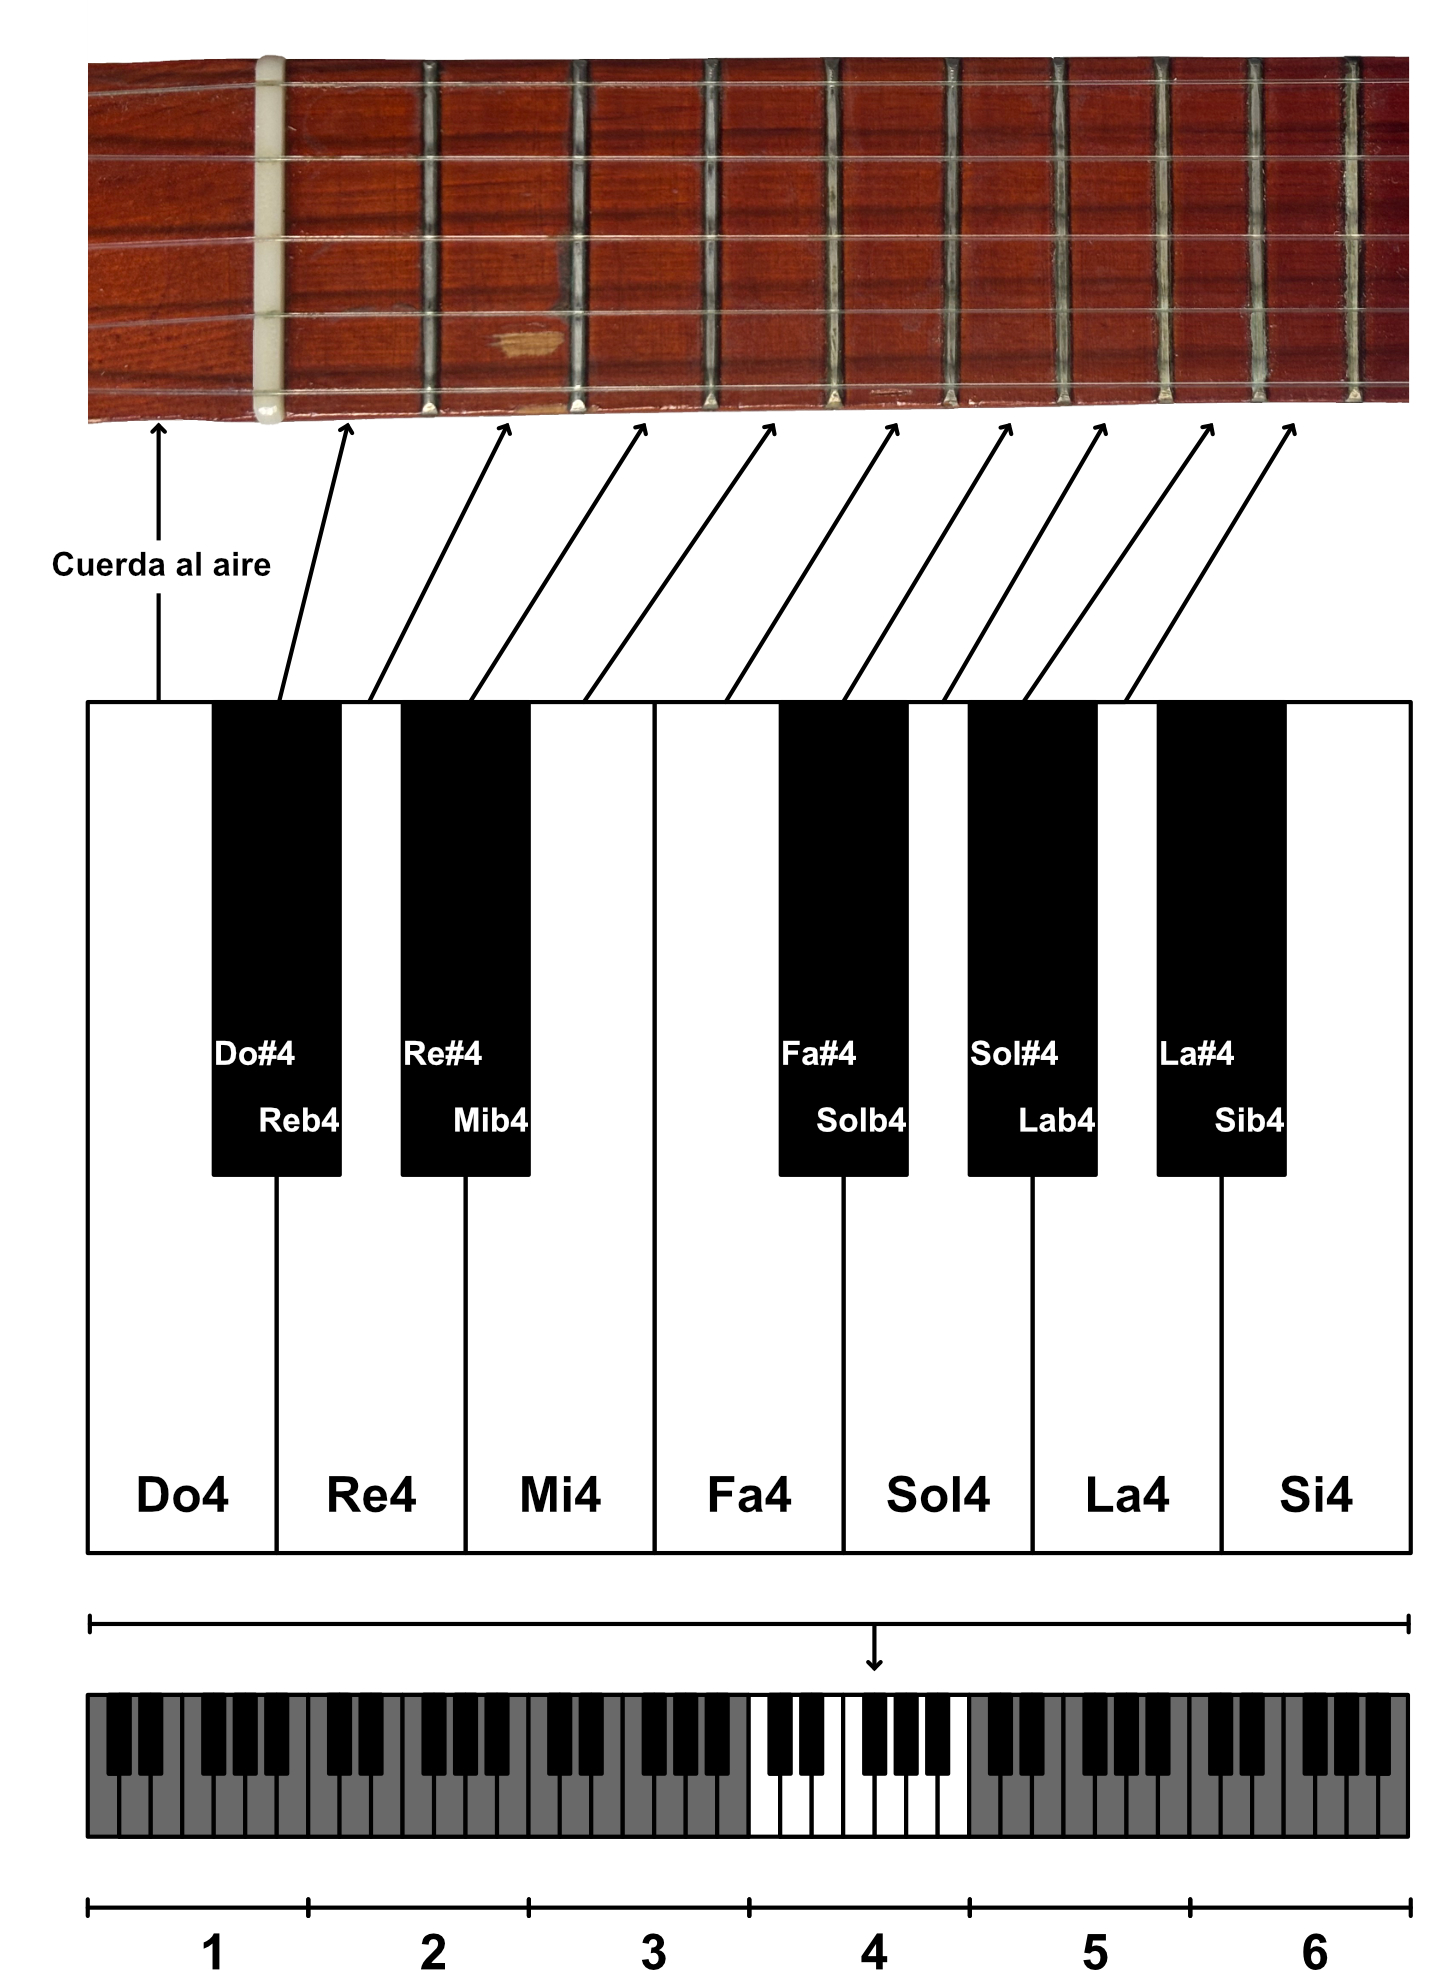
\includegraphics[width=\textwidth]{Ilustraciones/estado/timple_notas_piano.jpg}
        \caption{Relación entre notas del timple y el piano}
        \label{fig:timple_notas_piano}
    \end{subfigure}
    \caption{Comparación visual entre las partes del timple y su correspondencia con el piano.}
    \label{fig:timple_comparacion}
\end{figure}

Además, podemos instroducir el concepto \textbf{transposición de un instrumento}, que consiste en la transposición de todas las cuerdas al aire en un mismo número de semitonos.

Con respecto al toque de los instrumentos de cuerda pulsada, podemos distinguir dos técnicas:

\begin{itemize}
    \item El \textbf{\gls{punteo}}~\cite{wikipedia_punteo}, que consiste en el toque de notas individualmente.
    \item El \textbf{\gls{rasgueo}}~\cite{wikipedia_rasgueo}, que consiste en la reproducción de varias notas en forma de barrido, utilizando uno o mas dedos. Estos barridos se ejecutan siguiendo un patrón, existiendo una forma de representación a través de símbolos que indican la acción a ejecutar \tabref{tabla:simbolos_rasgueo}.
    \begin{table}[H]
        \centering
        \scriptsize
        \begin{tabular}{l c c c l}
            \hline
            \textbf{Rasgueo} & \multicolumn{3}{c}{\textbf{Símbolos}} & \textbf{Descripción} \\
            Abajo & $\downarrow$ & D & $\sqcap$ & Rasgueo hacia abajo (de cuerdas graves a agudas) \\
            Arriba & $\uparrow$ & U & $\vee$ & Rasgueo hacia arriba (de cuerdas agudas a graves) \\
            Percusión & $\times$ & $\times$ & $\times$ & Golpe de percusión o mute sobre la cuerda; se puede combinar con cualquier rasgueo \\
            \hline
        \end{tabular}
        \caption{Símbolos de rasgueo en instrumentos de cuerda pulsada}
        \label{tabla:simbolos_rasgueo}
    \end{table}
\end{itemize}

Finalmente, para la reproducción de canciones la notación en pentagrama es comunmente utilizada, pero existen ciertas notaciones diseñadas especificamente para este tipo de instrumentos:

\begin{itemize}
    \item La \textbf{\gls{tablatura}}~\cite{wikipedia_tablatura}, consiste en la representación gráfica de notas a través de una tabla \figref{fig:tablatura} donde cada linea horizontal equivale a una cuerda, los números equivalen a un traste y los simbolos indican efectos \tabref{tab:simbolos_tablatura}.
    
    \begin{table}[H]
        \centering
        \scriptsize
        \caption{Ejemplo de tablatura para timple}\label{fig:tablatura}
        \ttfamily
        \begin{tabular}{l l}
            Sol & |--0--2h--3--2--0-----------| \\
            Do  & |--2------------0-----------| \\
            Mi  & |--1------------2--2--2--2--| \\
            La  & |--2------------2-----------| \\
            Re  & |--0------------2-----------| \\
        \end{tabular}
    \end{table}

    \begin{table}[H]
        \centering
        \scriptsize
        \caption{Símbolos comunes de tablatura}\label{tab:simbolos_tablatura}
        \begin{tabular}{c l l}
            \hline
            \textbf{Símbolo} & \textbf{Nombre} & \textbf{Descripción} \\
            \hline
            h & Hammer & Se pulsa una nota martilleando con otro dedo sin volver a pulsar la cuerda \\
            p & Pull-off & Se suelta una nota dejando sonar una inferior ya pulsada \\
            / & Slide up & Deslizamiento hacia una nota más aguda \\
            \textbackslash & Slide down & Deslizamiento hacia una nota más grave \\
            b & Bend & Se estira la cuerda para subir la altura del sonido \\
            r & Release & Liberación del bend hacia la nota original \\
            $\sim$ & Vibrato & Pequeña oscilación continua en la nota \\
            t & Tapping & Percusión directa con un dedo de la mano derecha en el mástil \\
            \hline
        \end{tabular}
    \end{table}

    \item El \textbf{\gls{diagrama de acordes}}~\cite{imusicschool_diagramadeacordes}, consiste en la representación de los acordes a tocar sobre las palabras clave de la letra de una canción. Suele ir acompañado de una tabla donde las lineas verticales equivalen a las cuerdas y las horizontales a los trastes, utilizando circulos para indicar donde colocar los dedos~\figref{fig:diagrama_acordes}.
    
    \begin{figure}[H]
        \centering
        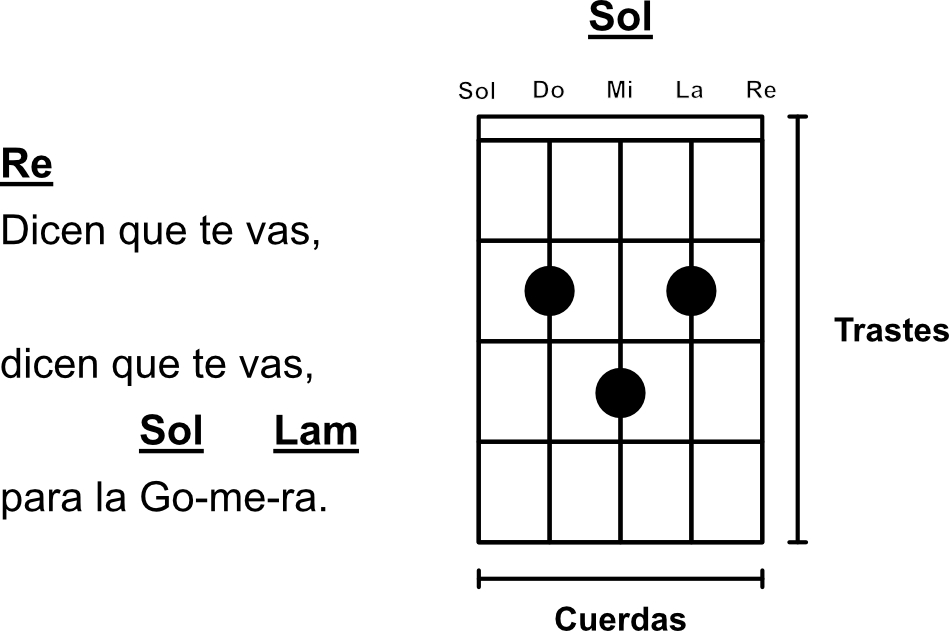
\includegraphics{Ilustraciones/estado/diagrama_acordes.jpg}
        \caption{Ejemplo de diagrama de acordes para timple}\label{fig:diagrama_acordes}
    \end{figure}
\end{itemize}
\subsection{Particularidades del timple}
\label{c:fundamentos_timple}

En su práctica, el timple se caracteriza por dos elementos:

\textbf{En primer lugar}, encontramos dos tipos de rasgueo:
\begin{itemize}
    \item El \textbf{tresillo}~\cite{pedroizquierdo_tresillo}, consistente en tres rasgueos seguidos, normalmente utilizando el índice y el pulgar. La secuencia suele ser: índice abajo, pulgar arriba y índice arriba.
    \item El \textbf{cinquillo}~\cite{pedroizquierdo_cinquillo}, consistente en cinco rasgueos seguidos, normalmente añadiendo a un rasgueo básico el tresillo. La secuencia suele ser: índice abajo, índice arriba, índice abajo, pulgar arriba, índice arriba.
\end{itemize}

\textbf{En segundo lugar}, dentro del folclore canario las \textbf{tonalidades}~\cite{timplismo_tonalidades}\cite{raquel_tonalidades_video} reciben un nombre propio \tabref{tab:tonalidades_timple}, siendo los grados I, IV, V7 los mas utilizados.

\begin{table}[H]
    \centering
    \scriptsize
    \begin{tabular}{l c c c}
    \hline
    \textbf{Nombre} & \textbf{I} & \textbf{IV} & \textbf{V7} \\
    \hline
    Tendío       & $DoM$ & $FaM$ & $Sol7$ \\
    Por el cinco & $ReM$ & $SolM$ & $La7$ \\
    Por el nueve & $MiM$ & LaM & Si7 \\
    La zorra     & $FaM$ & $SibM$ & $Do7$ \\
    Por el uno   & $SolM$ & $DoM$ & $Re7$ \\
    Por el seis  & $LaM$ & $ReM$ & $Mi7$ \\
    \hline
    \end{tabular}
    \caption{Tonalidades, grados y acordes con sus nombres folcloricos}\label{tab:tonalidades_timple}
\end{table}

\textbf{Además}, existe una variante del timple conocido como \textbf{contra} con afinación \textit{La, Mi, Si, Sol y Re}
\section{Estado Actual}
Encontrar información sobre un instrumento suele ser tan sencillo como realizar una búsqueda en internet. En el caso de \textbf{la guitarra y el ukelele}, los recursos son casi ilimitados gracias a la existencia de un gran número de páginas~(véase Figura~\ref{fig:cifra_isadecandidito}) y aplicaciones que cuentan con comunidades que crean y difunden contenido constantemente.

\begin{figure}[H]
    \centering
    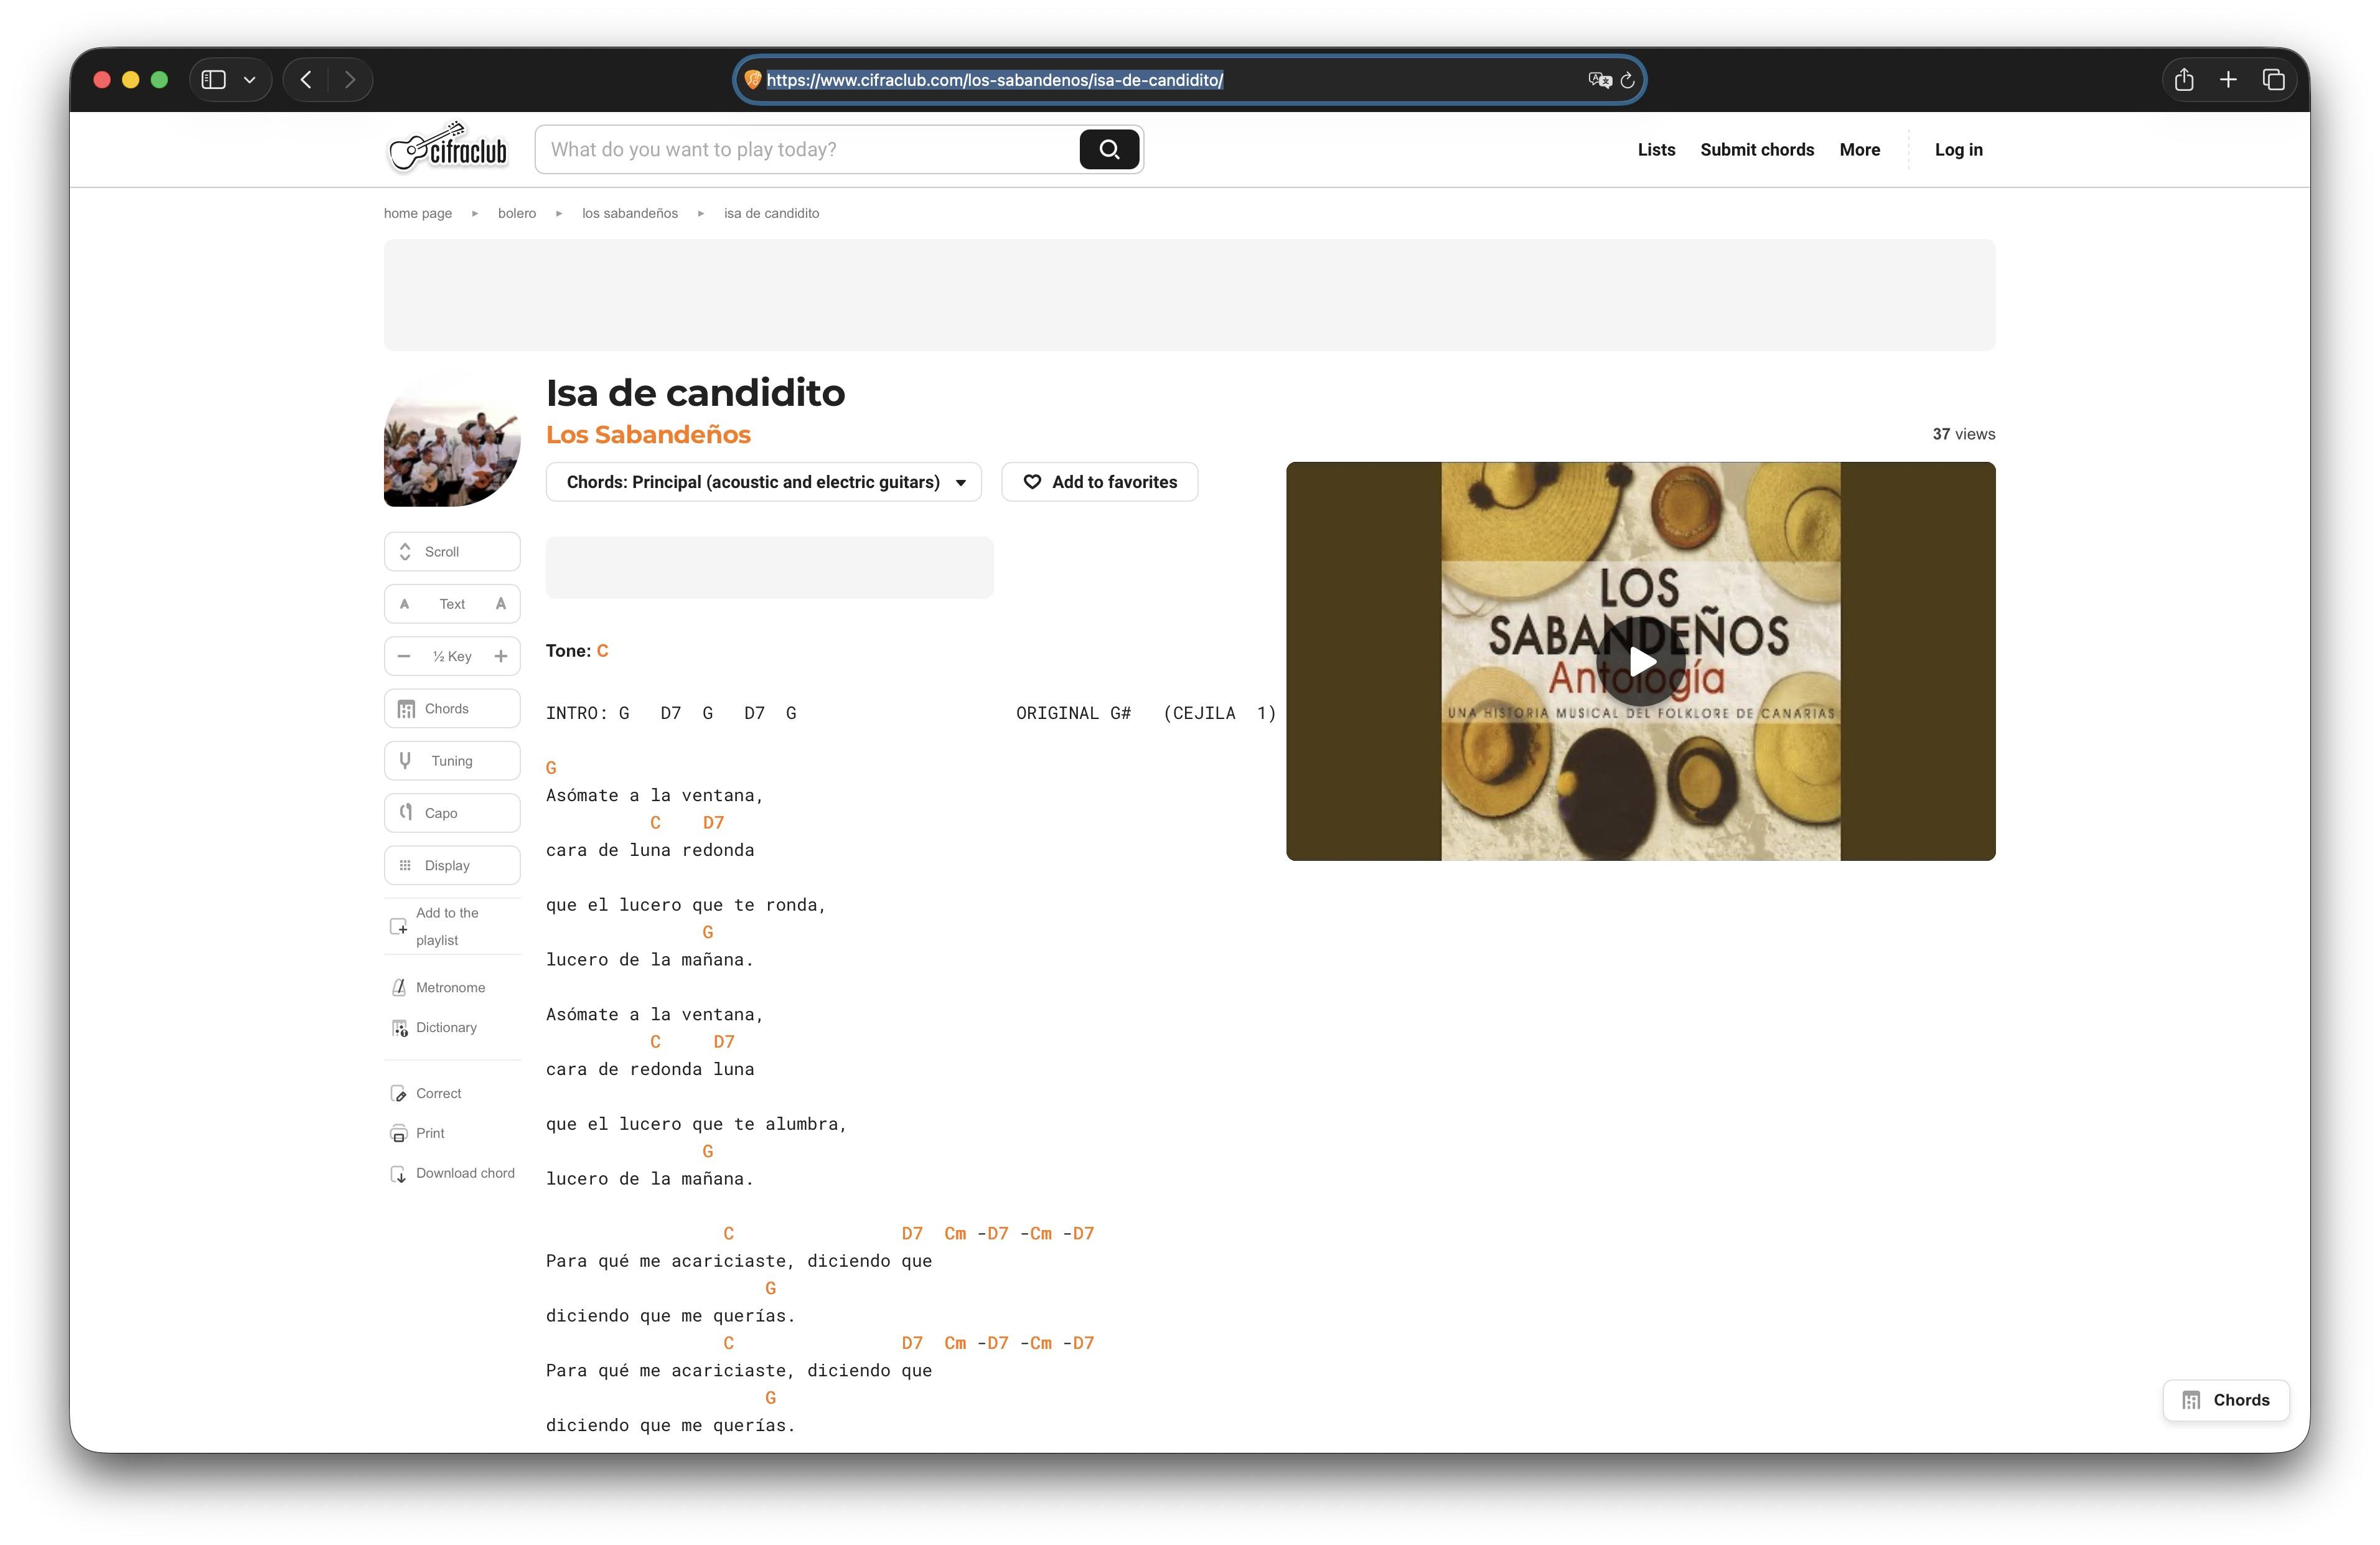
\includegraphics[width=0.80\textwidth]{Ilustraciones/estado/cifra_isadecandidito.jpeg}
    \caption{Letra y acordes de \emph{Isa de candidito} para guitarra en Cifra Club~\cite{cifra_isadecandidito}.}\label{fig:cifra_isadecandidito}
\end{figure}

Sin embargo, \textbf{el timple} no cuenta con las mismas facilidades. A diferencia de los instrumentos mencionados anteriormente, una simple búsqueda muestra cómo la información se encuentra dispersa en distintas plataformas, en su mayoría no especializadas:

\begin{itemize}
    \item \textbf{Redes Sociales}, siendo su principal medio de difusión. Podemos encontrar distintos perfiles, incluyendo comerciales \emph{(i.e. autores promocionando canciones, o profesores dando a conocer recursos o cursos de pago)}, así como perfiles didácticos y de aficionados. Destacamos a Raquel Álvarez que a través de la plataforma \textbf{YouTube} realiza una gran labor divulgativa mediante la enseñanza de técnicas para timple (véase Figura~\ref{fig:raquel_youtube_video}).
    
    \item \textbf{Páginas Web}, donde distinguimos:
    \begin{itemize}
        \item \textbf{Espacios dedicados a otros instrumentos}, con canciones que pueden ser reproducidas en el timple.
        \item \textbf{Páginas promocionales de cursos o recursos}, mayormente de pago. Destacamos a Pedro Izquierdo que a través de su página web ofrece servicios como cursos, herramientas y partituras (algunas gratuitas) (véase Figura~\ref{fig:pedro_izquierdo_pagina_partituras}).
    \end{itemize}
    
    \item \textbf{Libros}, mayormente físicos, de gran antigüedad o incluso inaccesibles actualmente.
\end{itemize}

\begin{figure}[H]
    \centering
    % Primera subfigura
    \begin{subfigure}[b]{0.48\textwidth}
        \centering
        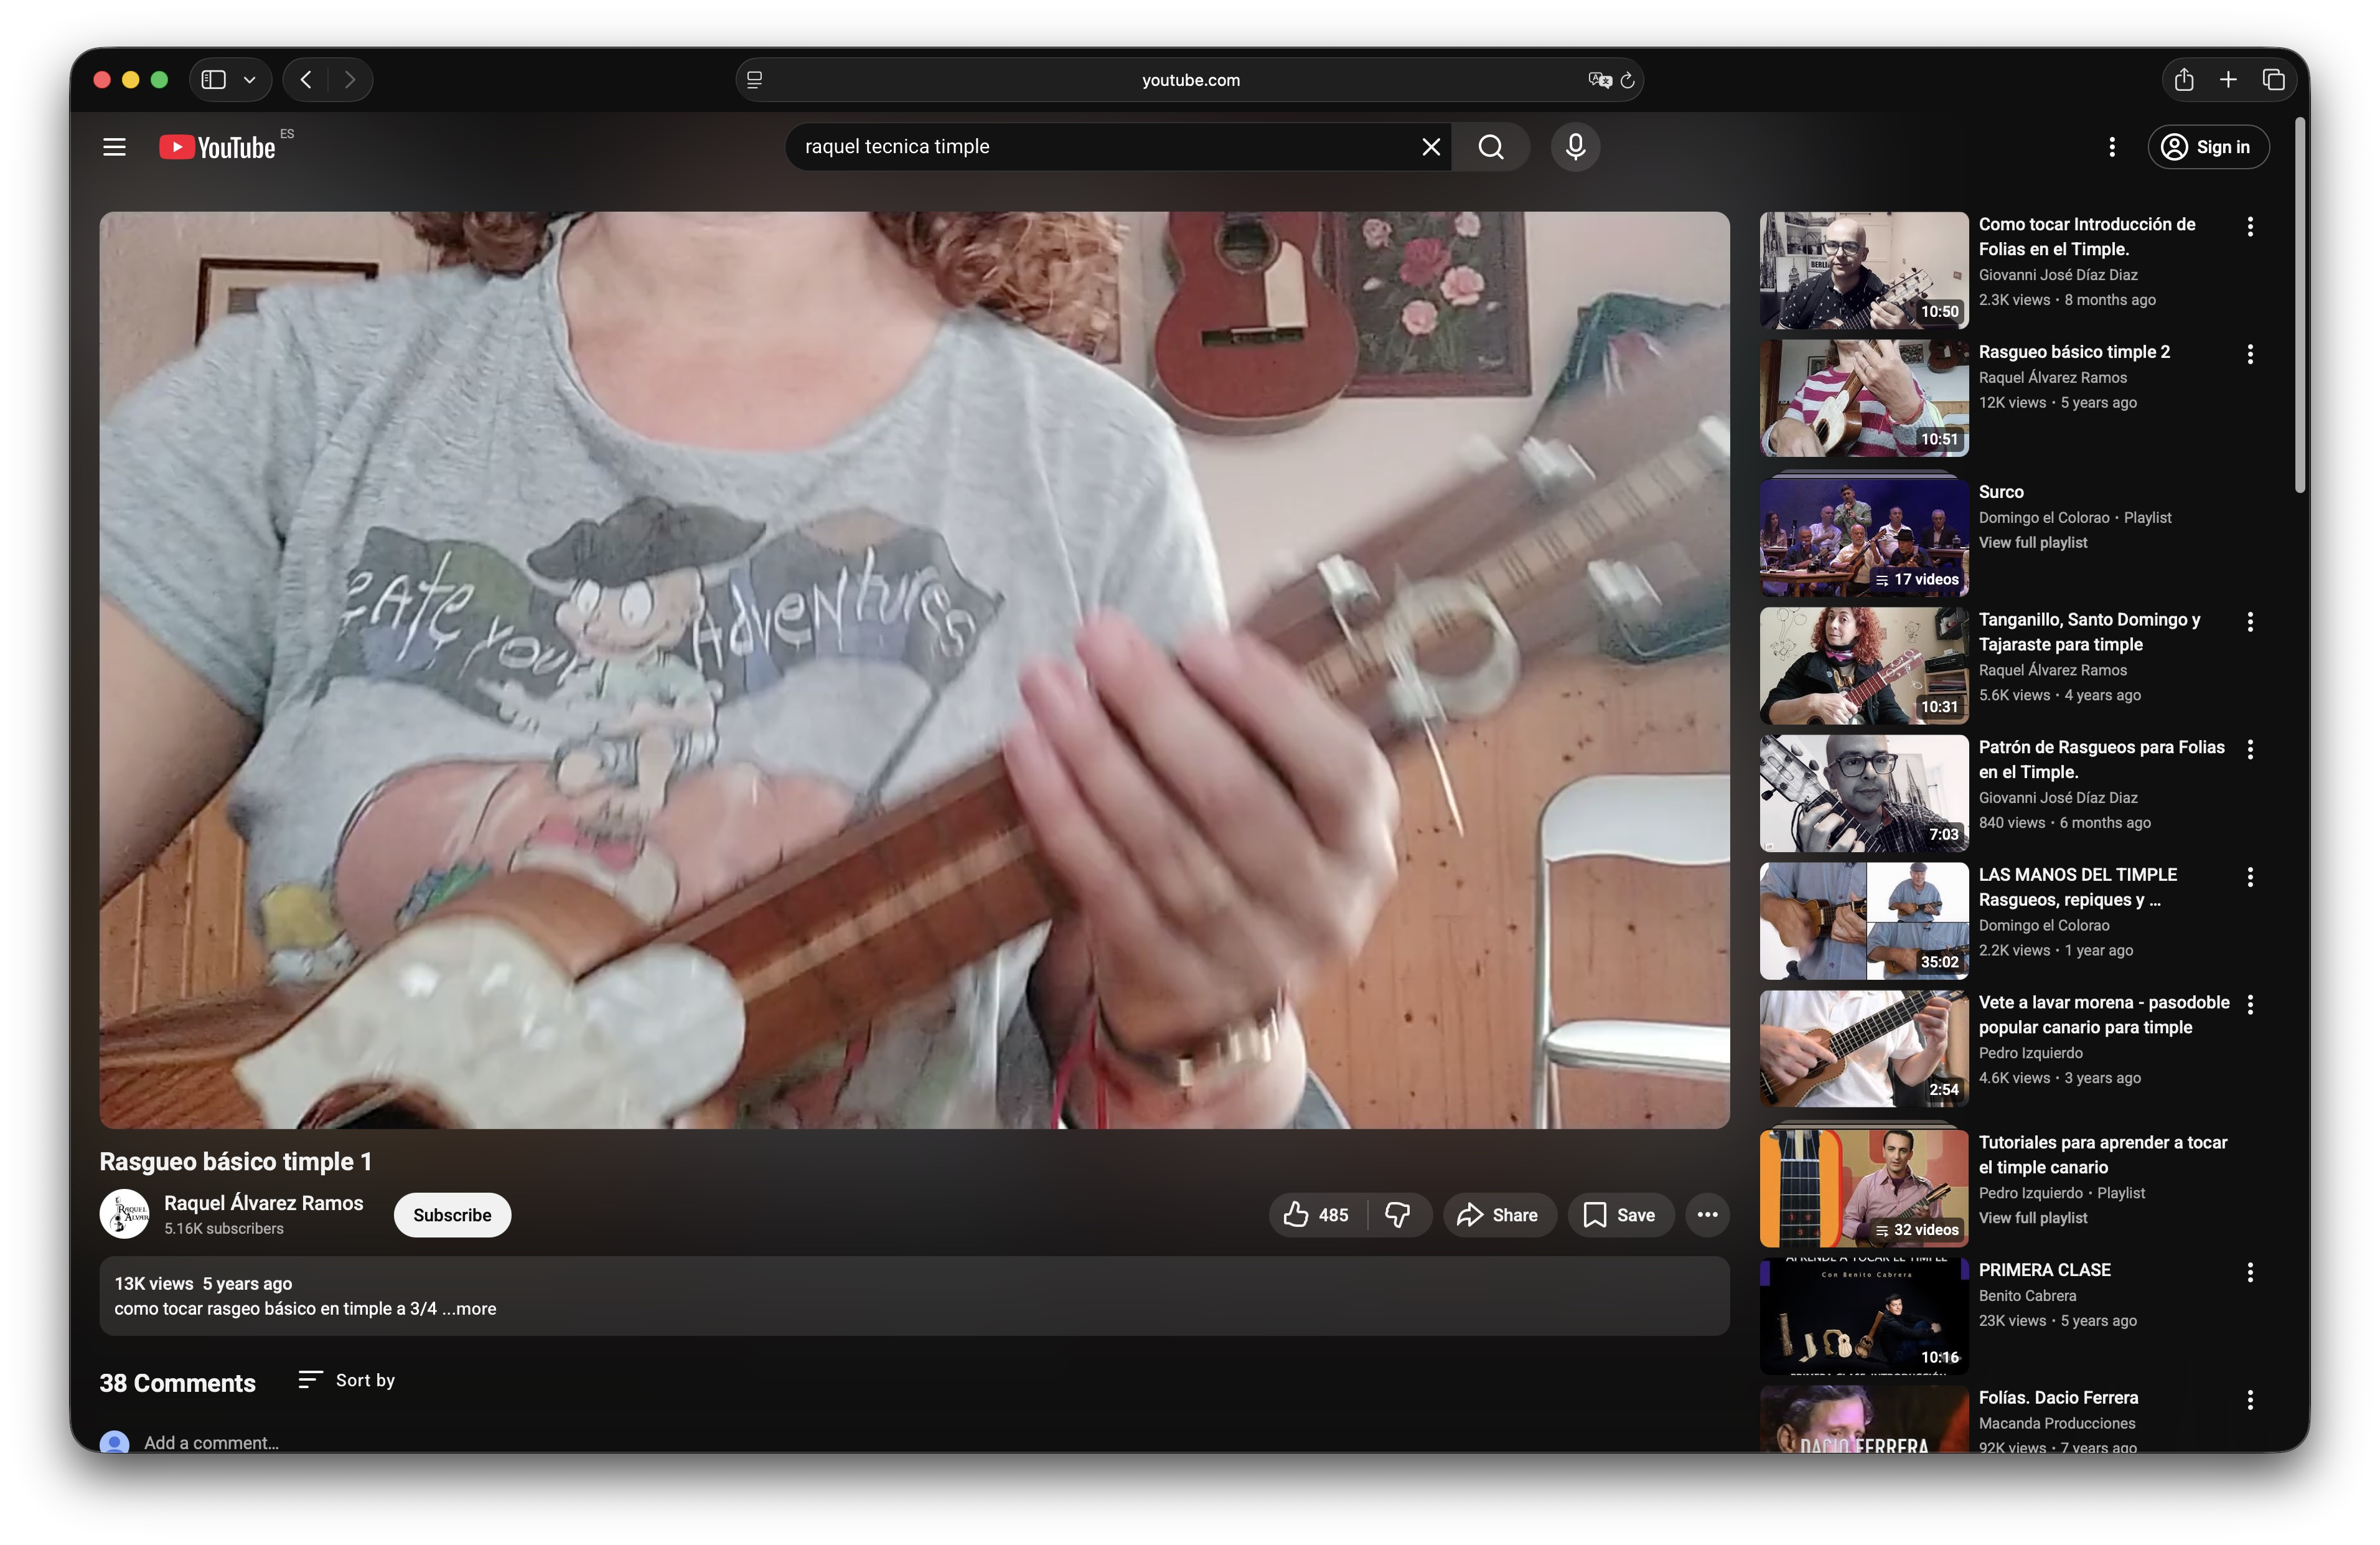
\includegraphics[width=\textwidth]{Ilustraciones/estado/raquel_youtube_video.jpeg}
        \caption{Video de \emph{Rasgueo básico timple 1} por Raquel Álvarez~\cite{raquel_youtube_video}}\label{fig:raquel_youtube_video}
    \end{subfigure}
    \hfill
    % Segunda subfigura
    \begin{subfigure}[b]{0.48\textwidth}
        \centering
        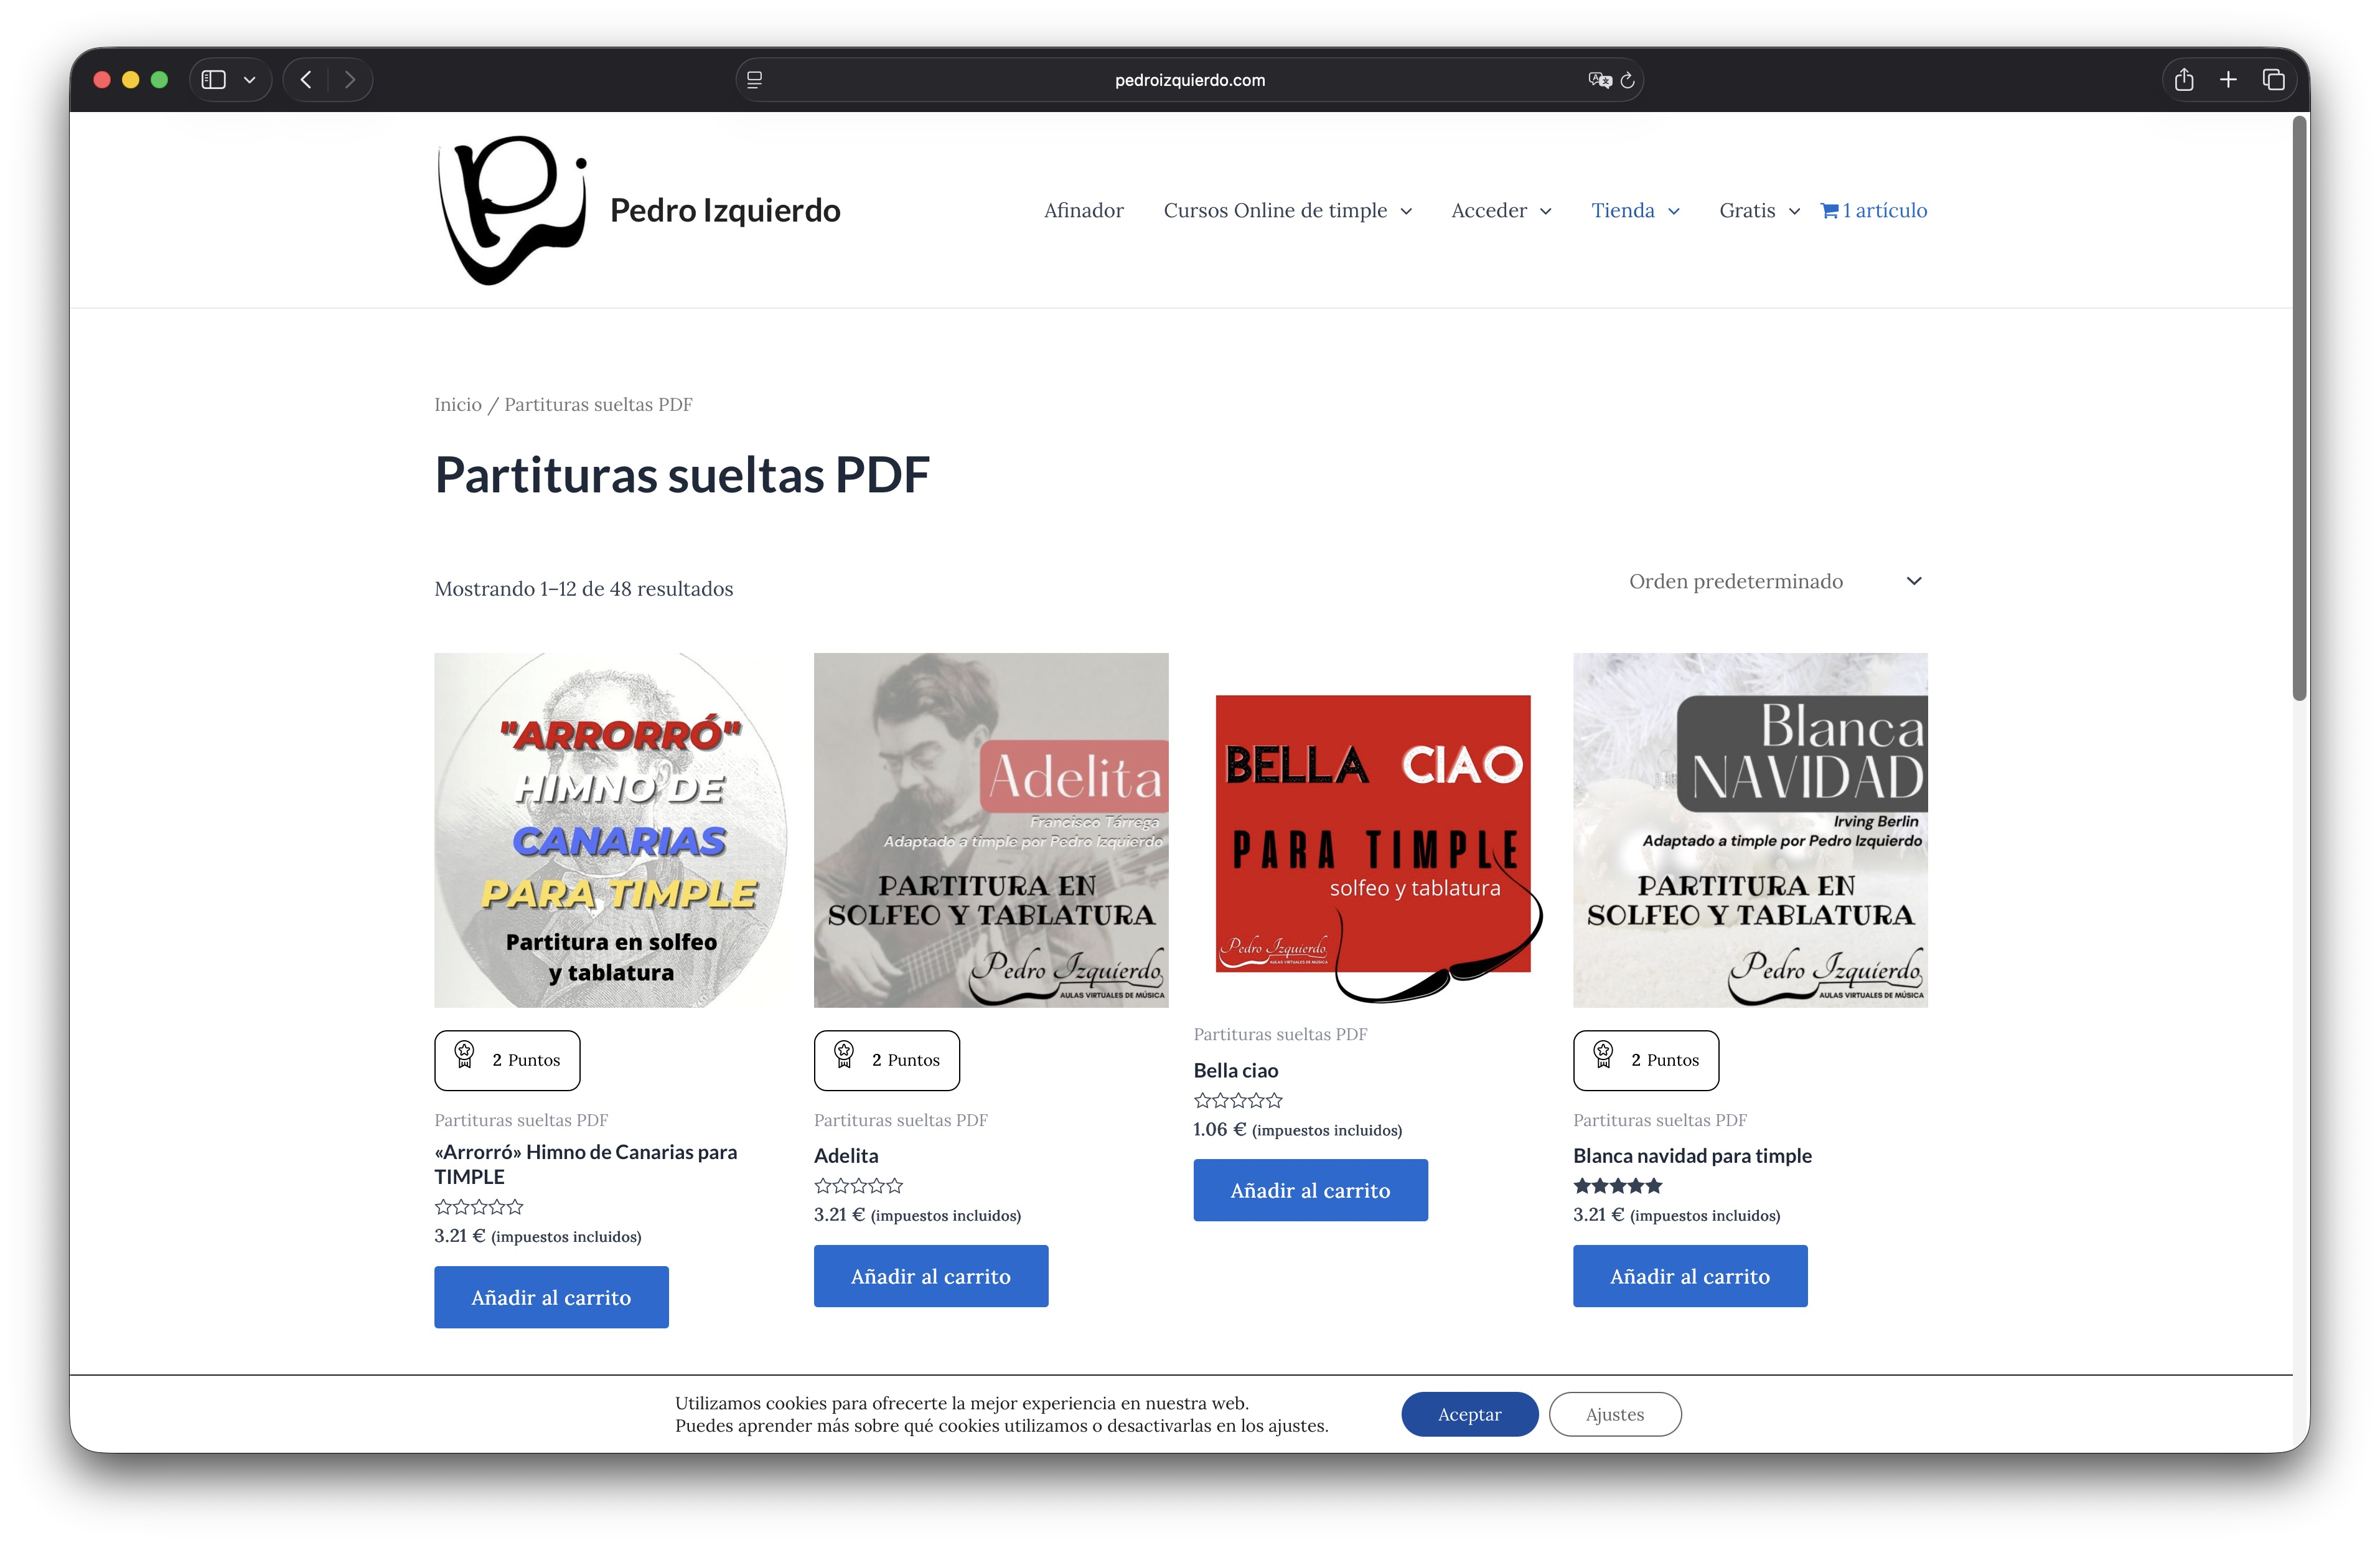
\includegraphics[width=\textwidth]{Ilustraciones/estado/pedro_izquierdo_pagina_partituras.jpeg}
        \caption{Partituras por Pedro Izquierdo en su página web~\cite{pedro_izquierdo_pagina_partituras}}\label{fig:pedro_izquierdo_pagina_partituras}
    \end{subfigure}
    % Caption general
    \caption{Recursos para timple en distintas plataformas digitales.}\label{fig:comparacion_timple}
\end{figure}

%Concluimos que, a diferencia de otros instrumentos, no existe un espacio digital dedicado exclusidamente al timple. Además, su comunidad se encuentra activa, pero dispersa en distintas plataformas. 

%Dada la escasez de alternativas y recursos, se abre la oportunidad de crear una aplicación web diseñada para el timple, poniendo a su comunidad como foco y ofreciendo todas las utilidades necesarias para la creación, difusión y práctica de canciones.

En conclusión, la comunidad del timple se encuentra fragmentada en distintas plataformas, con escasos recursos (en algunos casos antiguos o incluso inaccesibles) y sin un espacio propio. Estas necesidades no cubiertas y la existencia de alternativas exitosas para otros instrumentos, abren paso a la oportunidad para la creación de una aplicación web especificamente diseñada para este instrumento.
\section{Análisis de aplicaciones web}
Aunque no especificamente para el timple, existen un gran número de aplicaciones web dedicadas a la creación difusión y práctica de canciones para otros instrumentos. A continuación se describen algunas de las aplicaciones webs mas populares, dedicadeas especificamente al ukelele y a la guitarra.

\subsection{Ukulele Tabs}

Ukulele Tabs es una aplicación web dedicada exclusivamente al ukelele. Entre las páginas que componen la aplicación distinguimos las relacionadas con canciones, herramientas y las informativas.

En primer lugar, con respecto a las \textbf{páginas relacionadas con canciones}, podemos encontrar:

\begin{itemize}
    \item \textbf{Biblioteca de canciones} (véase Figura~\ref{fig:ukuleletabs_home}), con la posibilidad de realizar búsquedas avanzadas por género, artista, popularidad, dificultad, año o país.
    \item \textbf{Canciones} (véase Figura~\ref{fig:ukuleletabs_somewhereovertherainbow}) que contienen la letra, acordes y utilidades (véase Tabla~\ref{tab:ukuleletabs_utilidades_canciones}) para la práctica de las mismas.
    

    \item \textbf{Solicitudes} de nuevas canciones.
\end{itemize}

En segundo lugar, en cuanto a las \textbf{páginas de herramientas e informativas}, distinguimos:

\begin{itemize}
    \item \textbf{Cursos} (véase Figura~\ref{fig:ukuleletabs_lecciones}), con publicaciones destinadas a la enseñanza del instrumento, principios básicos musicales y técnicas intermedias y avanzadas.
    \item \textbf{Diccionario de acordes}, con un listado de tablas con diagramas de acordes.
    \item \textbf{Calculadora de escalas y notas} (véase Figura~\ref{fig:ukuleletabs_escalas}), que muestra la ubicación de las notas en una simulación del mástil del instrumento.
    \item  \textbf{Bibliotecas de sonido} para escuchar rasgueos y afinar el instrumento a oído.
\end{itemize}

\begin{figure}[H]
    \centering
    % Primera subfigura
    \begin{subfigure}[t]{0.48\textwidth}
        \centering
        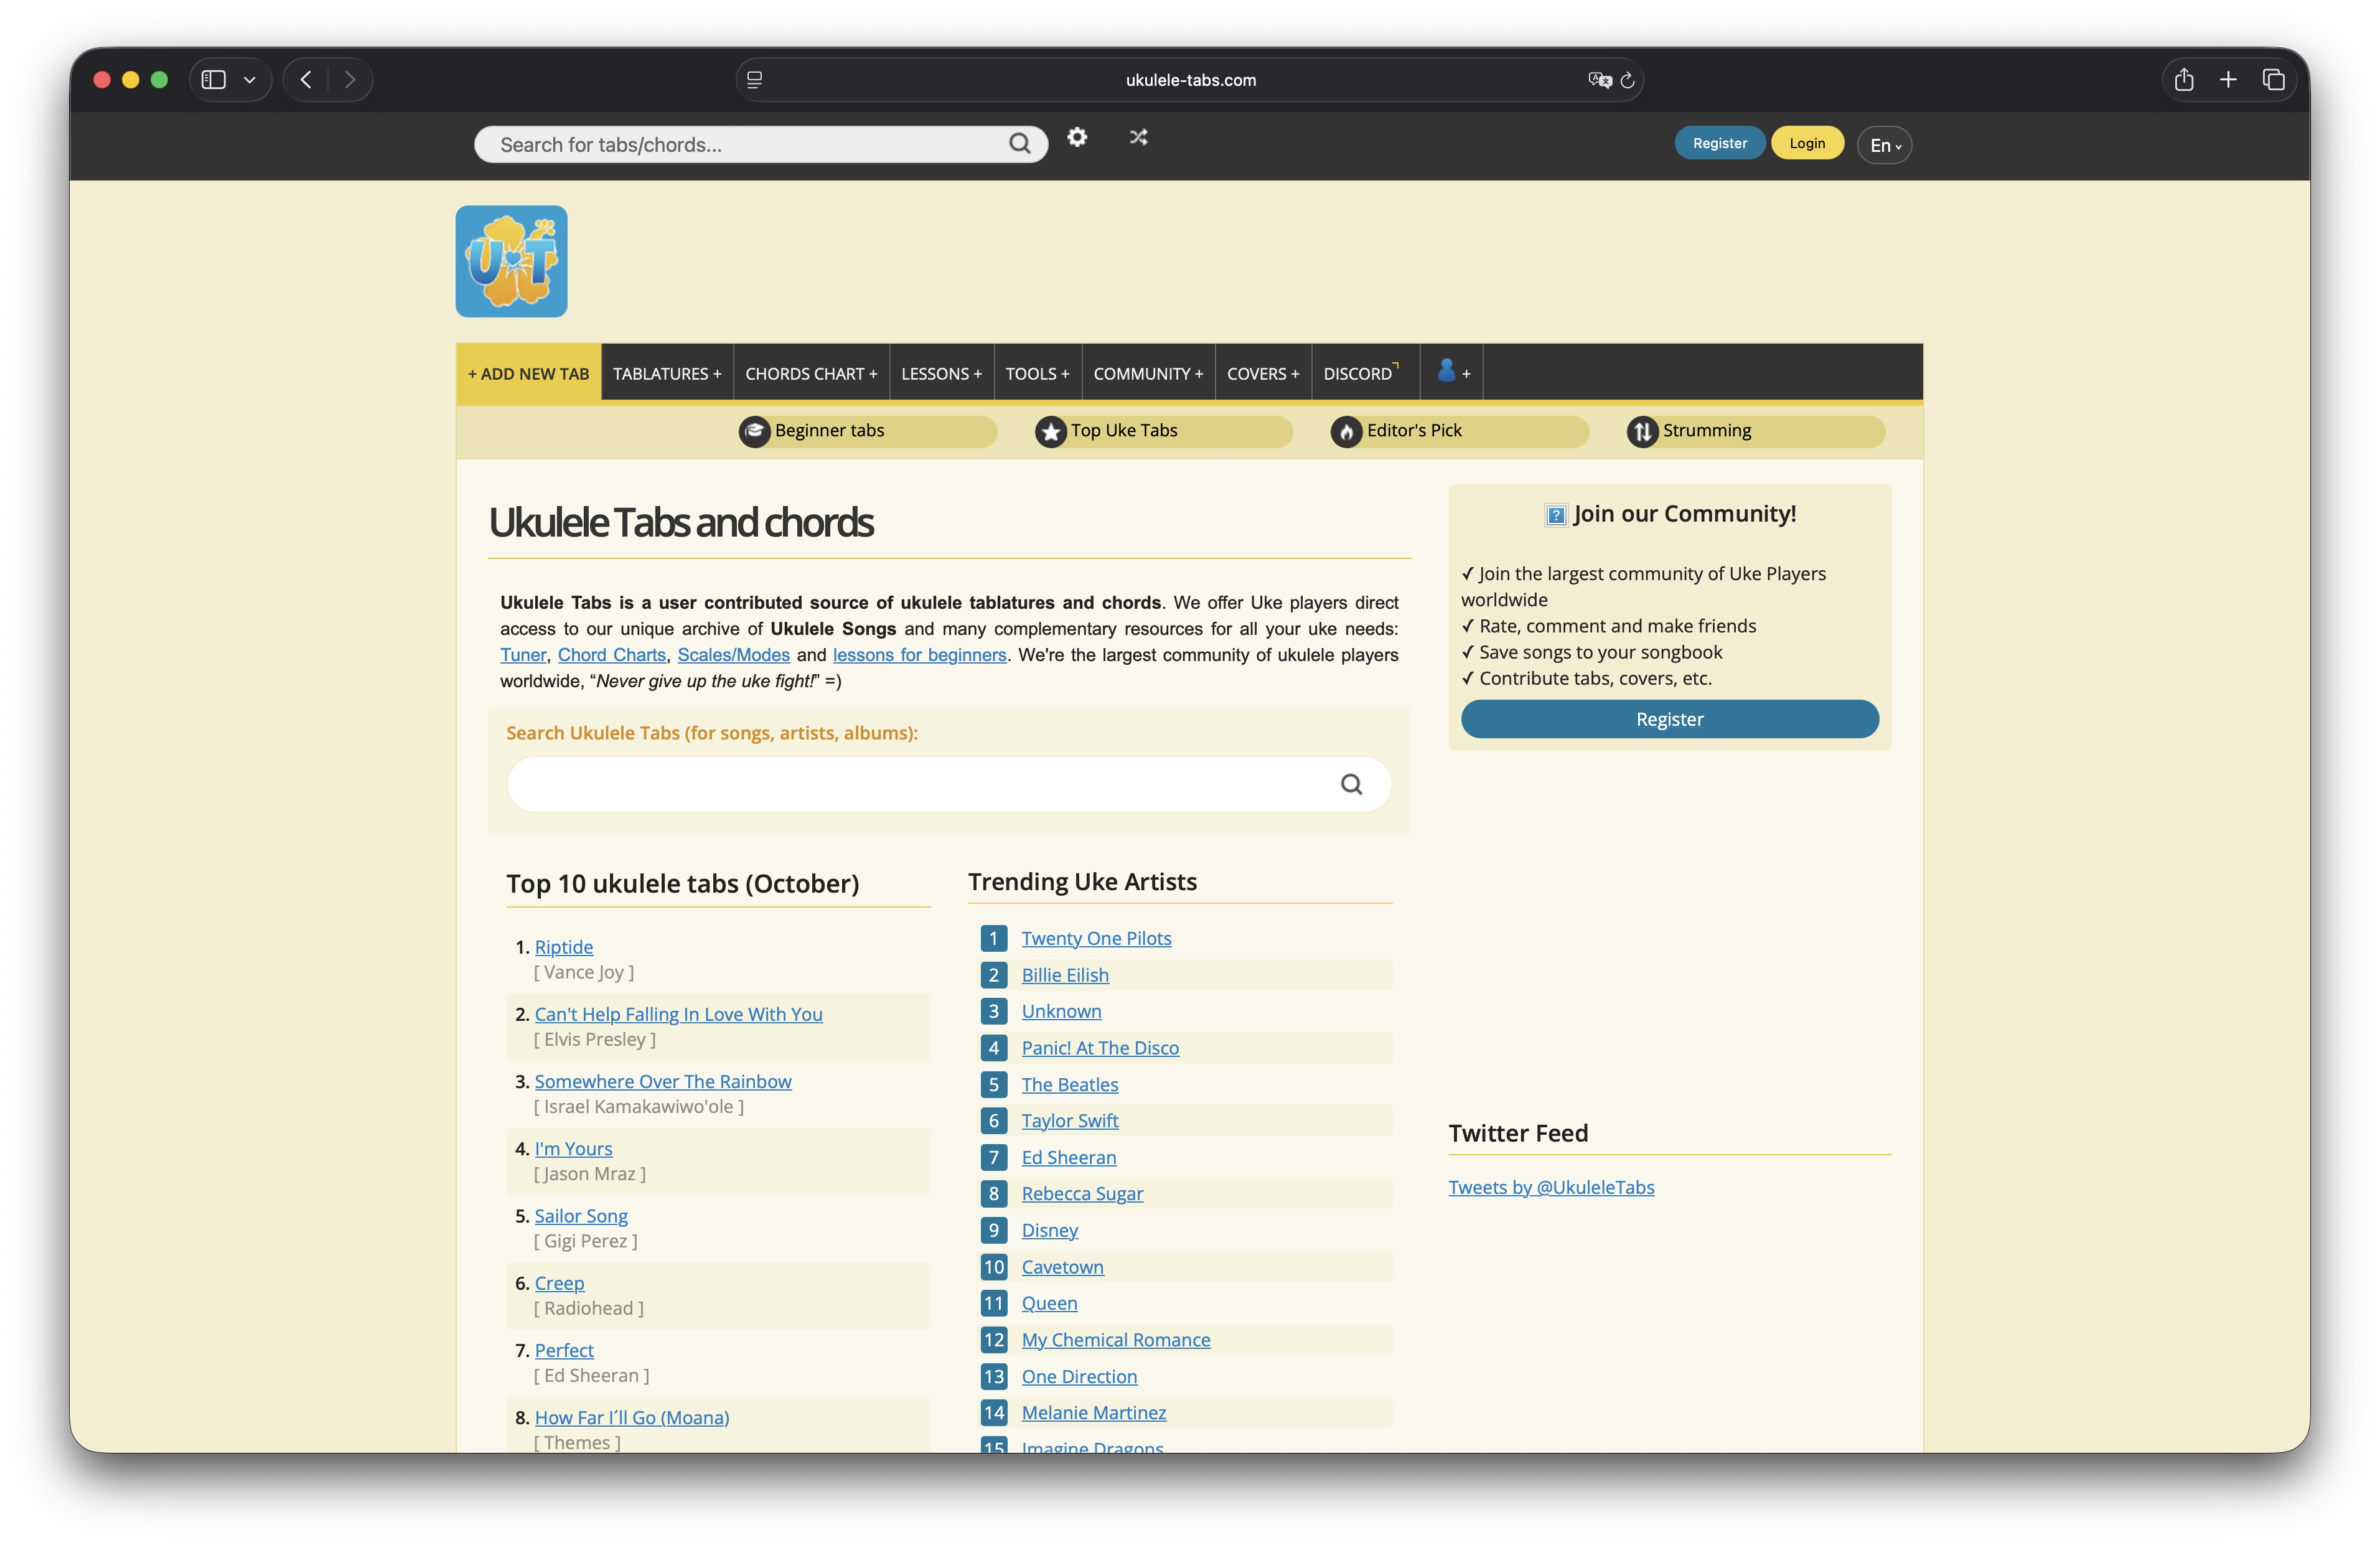
\includegraphics[width=\textwidth]{Ilustraciones/estado/ukuleletabs.jpeg}
        \caption{Página principal de Ukulele Tabs~\cite{ukuleletabs_home}}\label{fig:ukuleletabs_home}
    \end{subfigure}\hfill
    \begin{subfigure}[t]{0.48\textwidth}
        \centering
        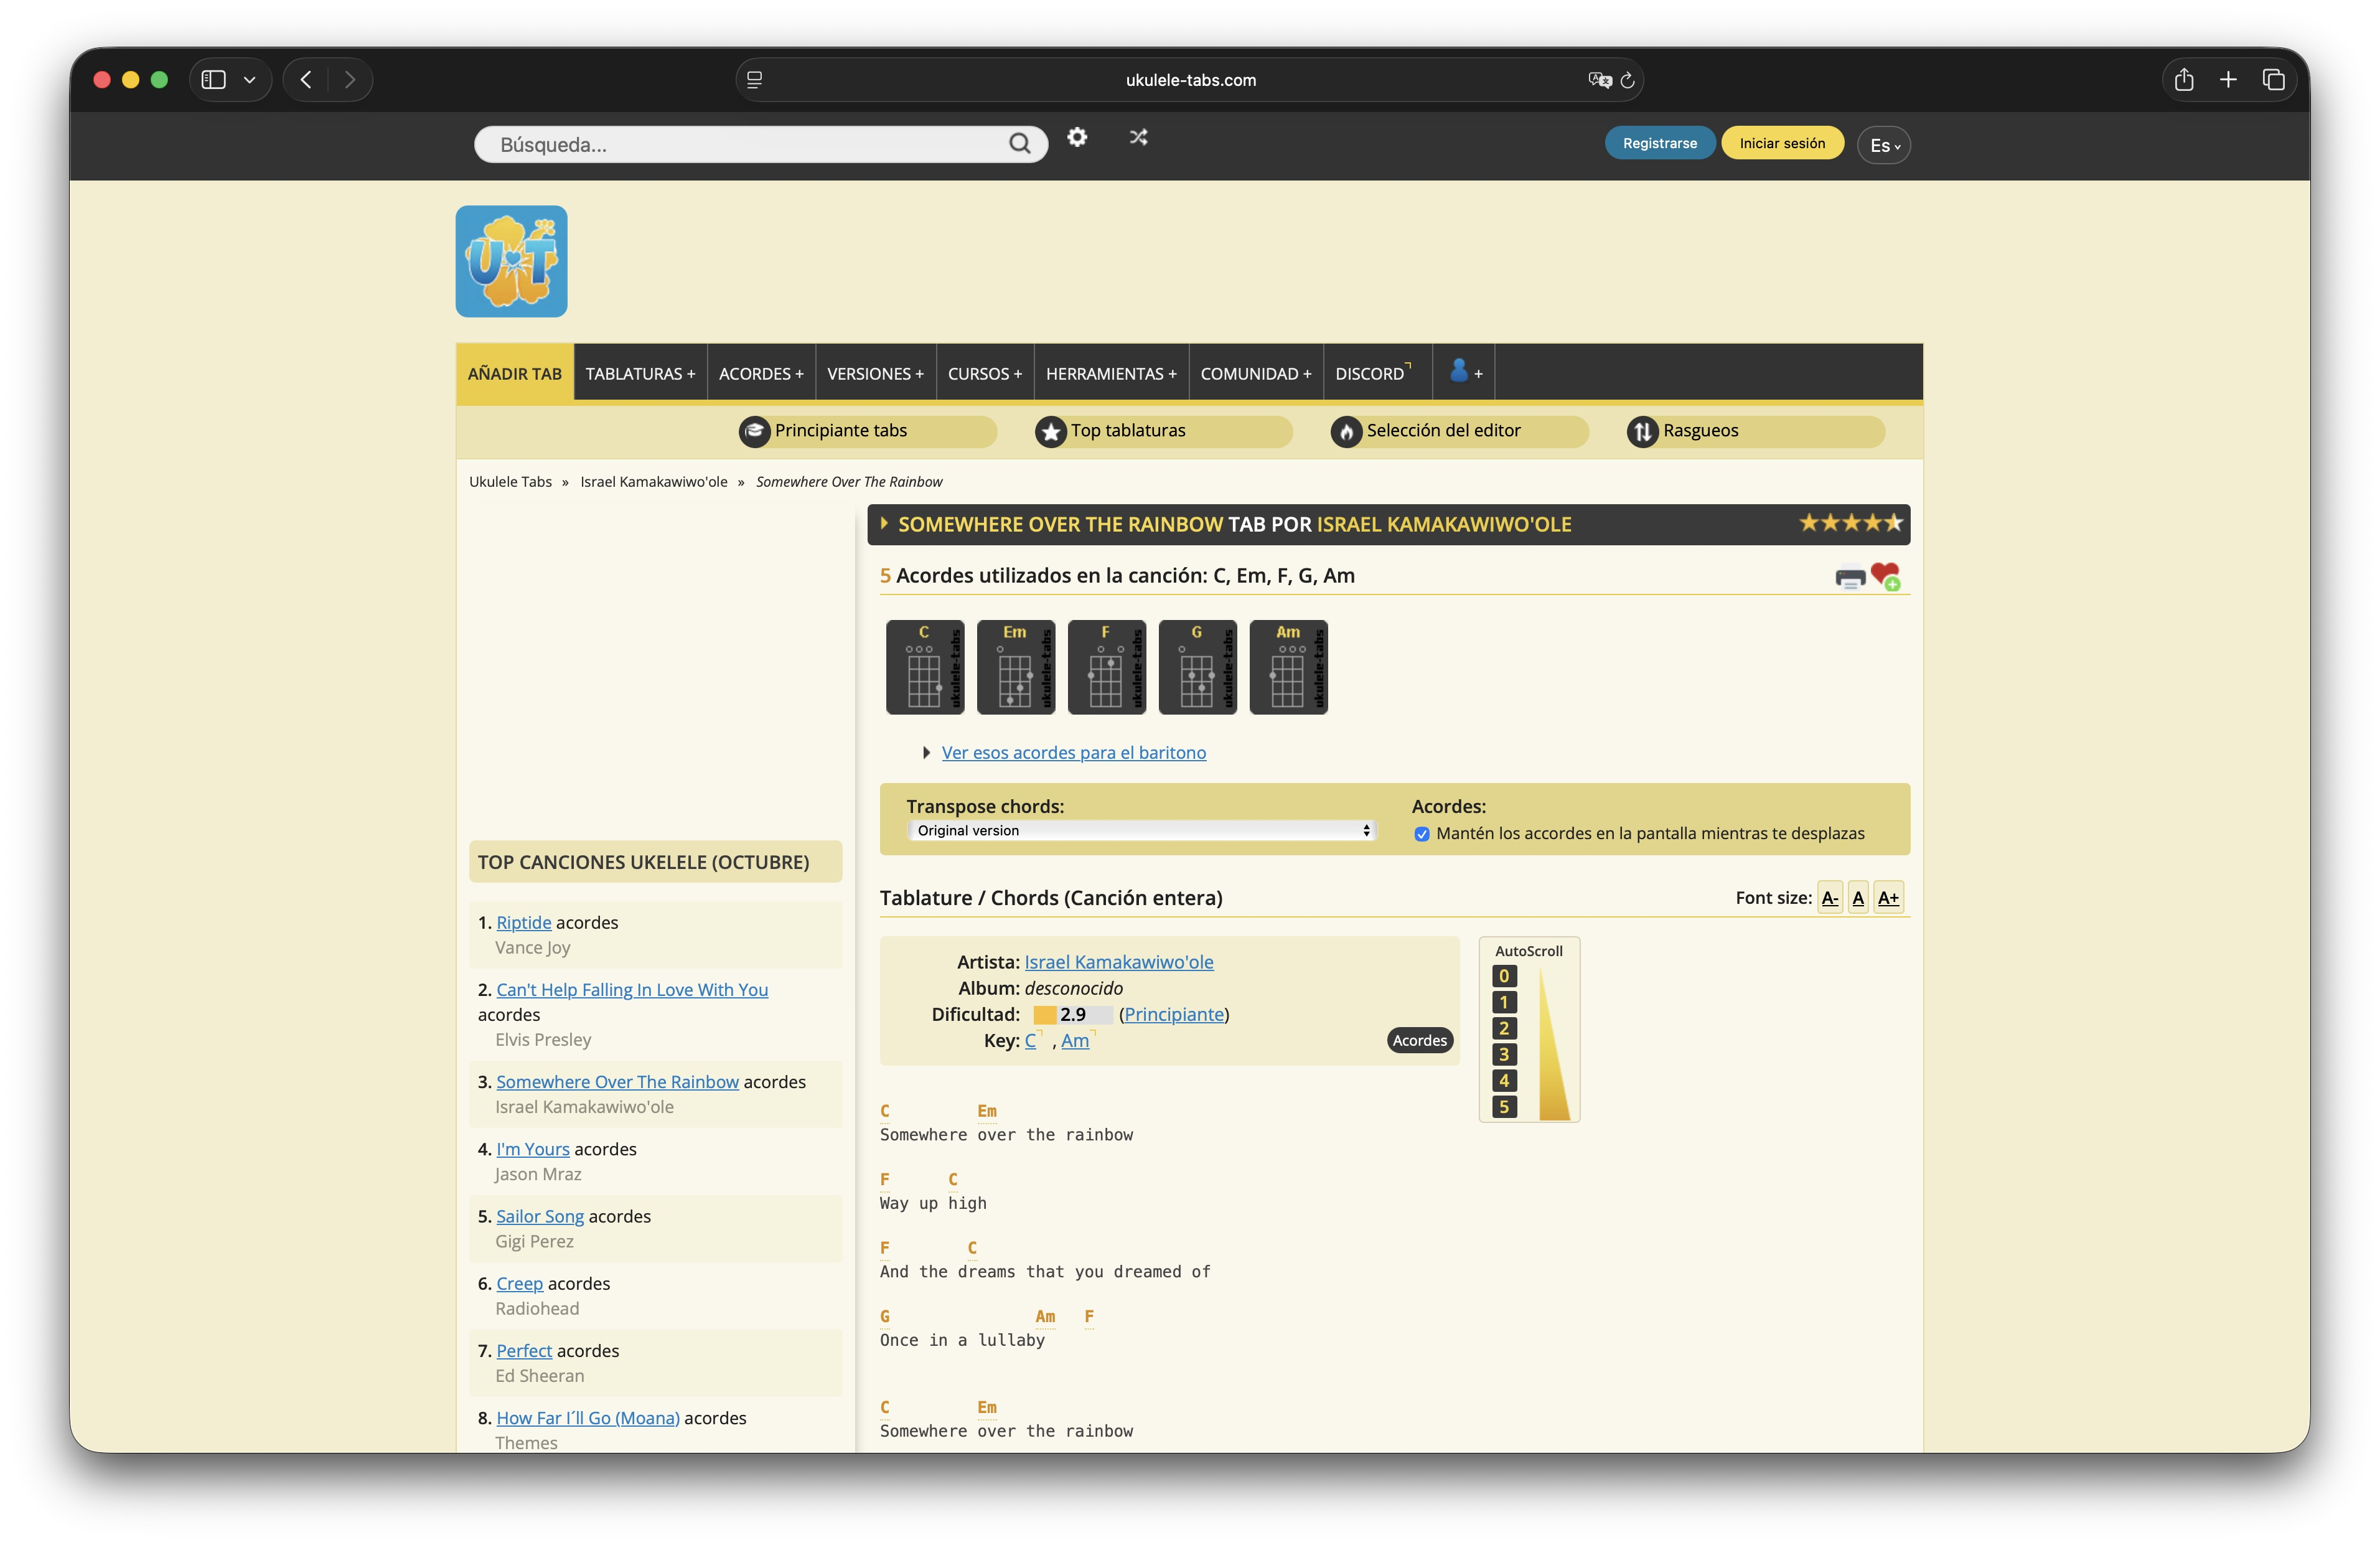
\includegraphics[width=\textwidth]{Ilustraciones/estado/ukuleletabs_somewhereovertherainbow.jpeg}
        \caption{Acordes y letra de \emph{Somewhere over the rainbow} para ukelele en Ukulele Tabs~\cite{ukuleletabs_somewhereovertherainbow}}\label{fig:ukuleletabs_somewhereovertherainbow}
    \end{subfigure}
    \vspace{1em} % Espacio vertical entre filas

    % segunda subfigura
    \begin{subfigure}[t]{0.48\textwidth}
        \centering
        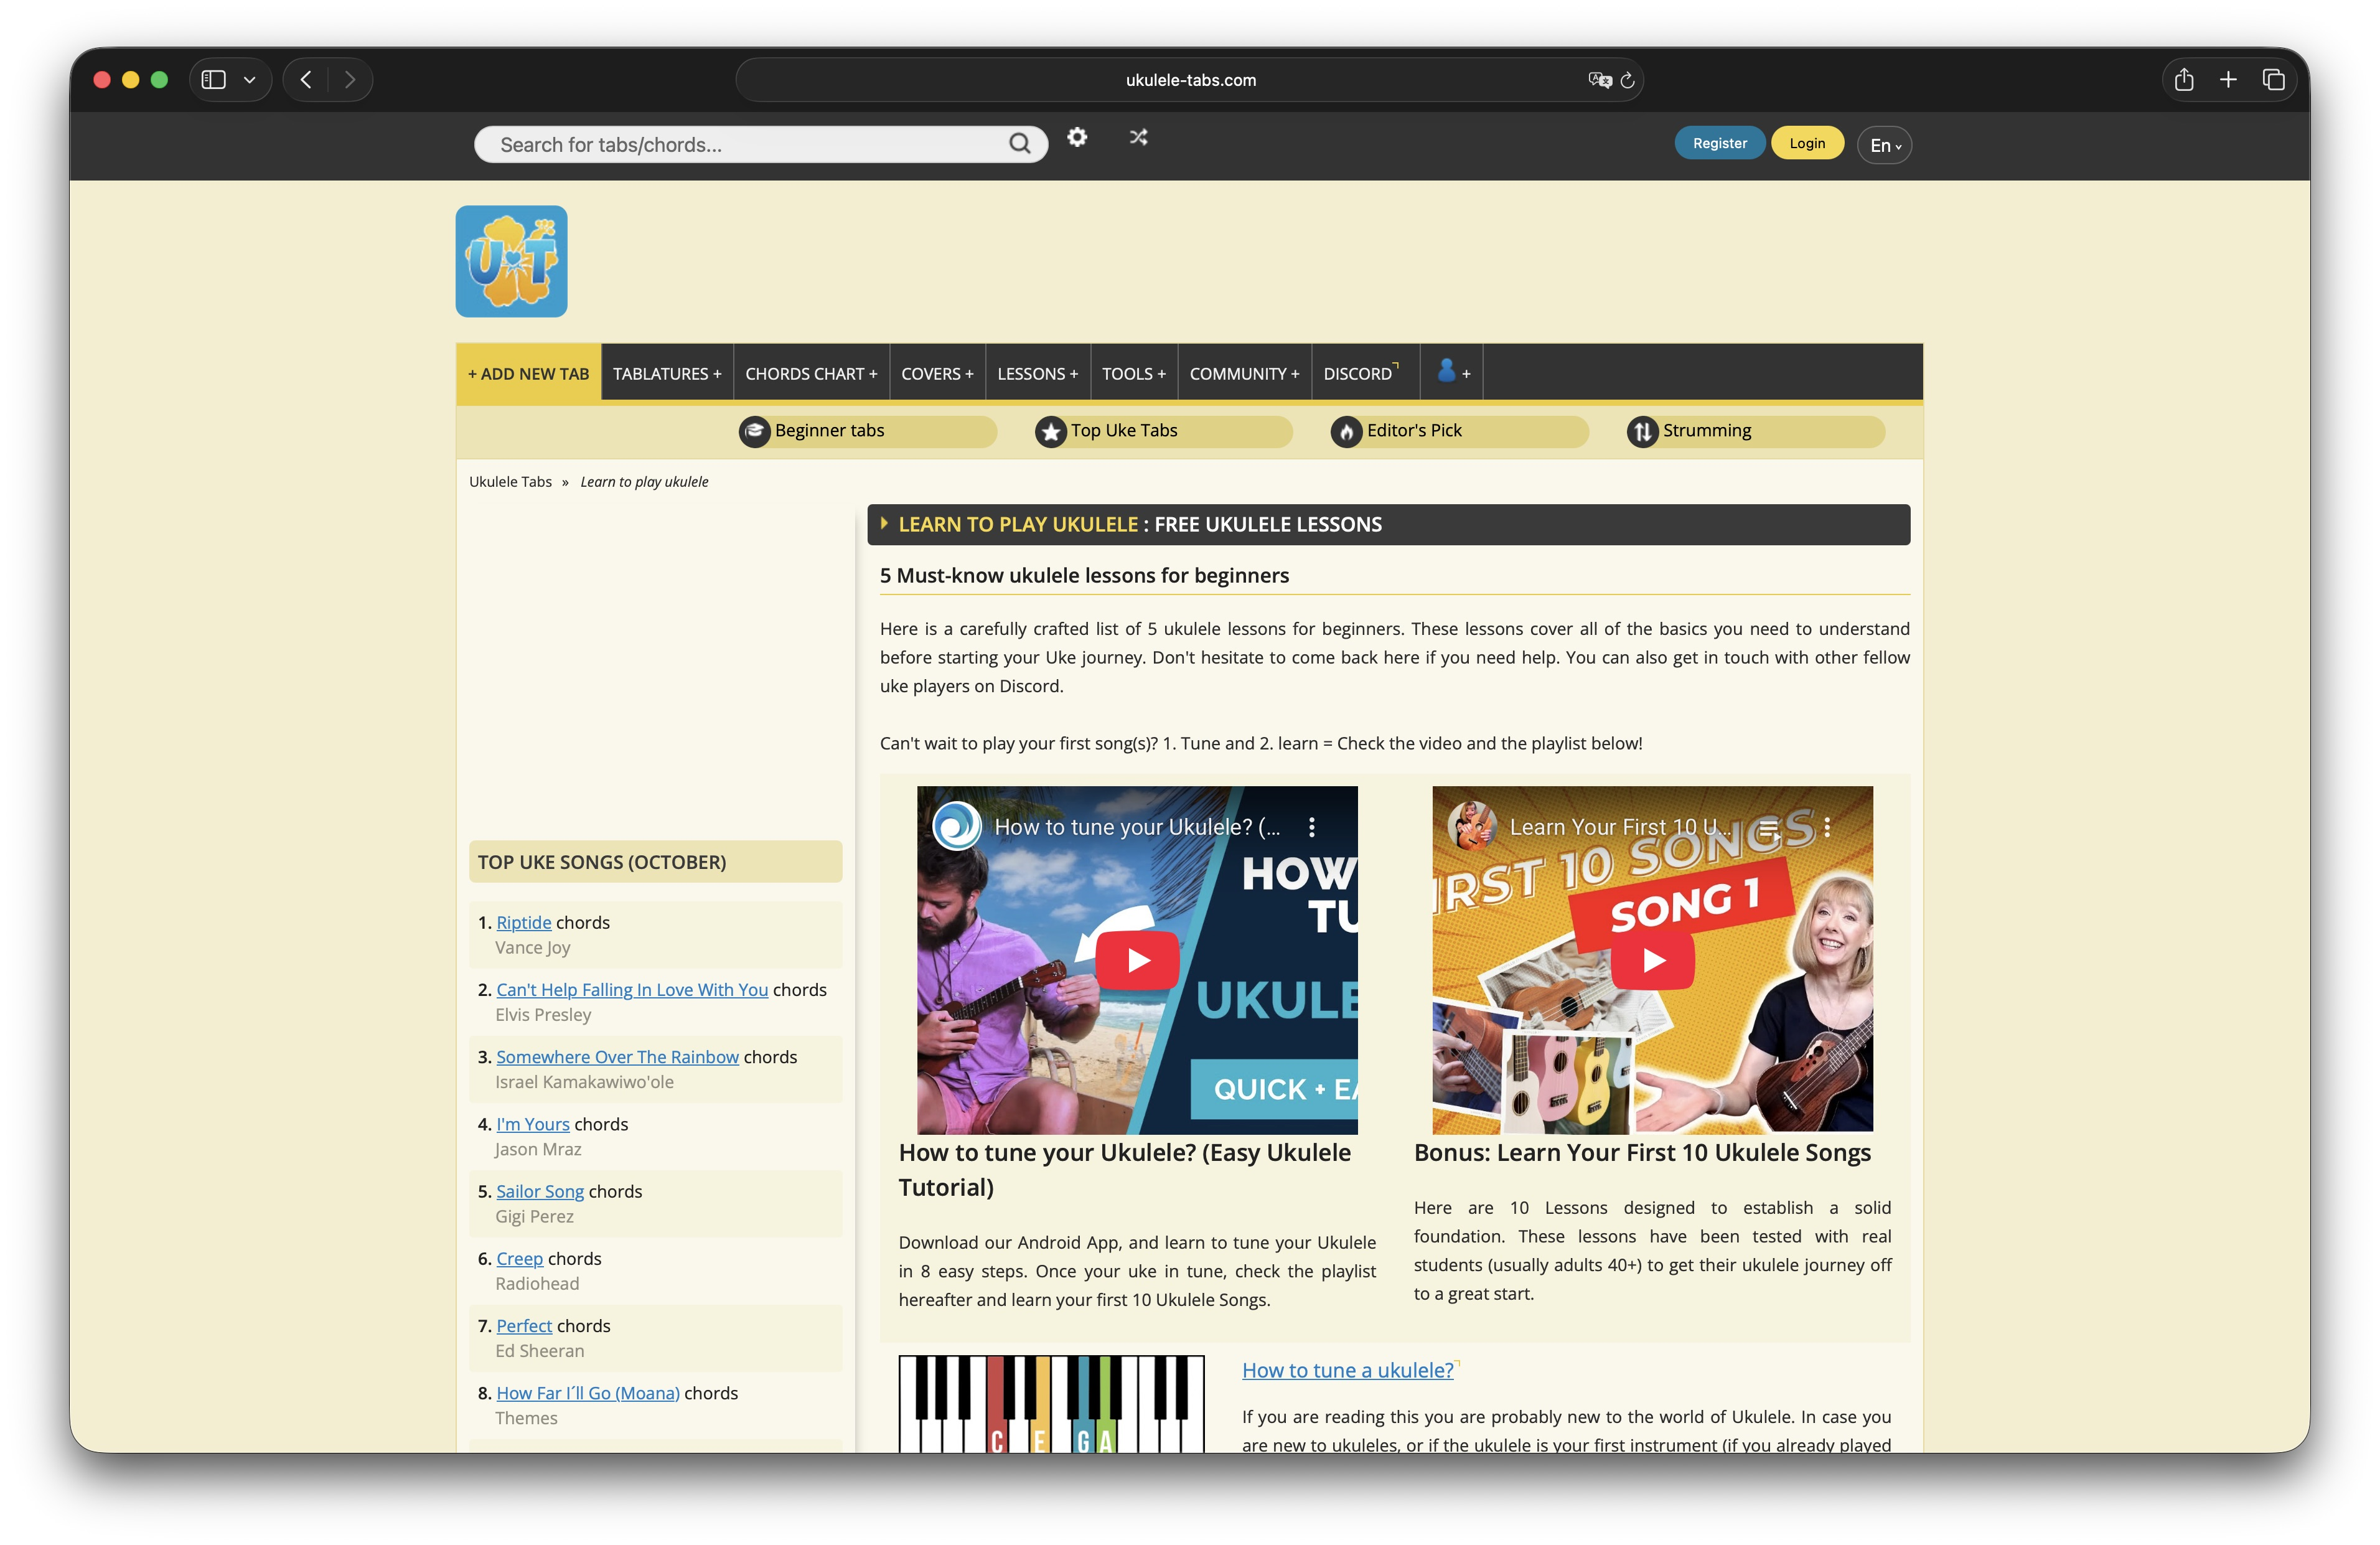
\includegraphics[width=\textwidth]{Ilustraciones/estado/ukuleletabs_lessons.jpeg}
        \caption{Página de cursos de Ukulele Tabs~\cite{ukuleletabs_lecciones}}\label{fig:ukuleletabs_lecciones}
    \end{subfigure}\hfill
    % segunda subfigura
    \begin{subfigure}[t]{0.48\textwidth}
        \centering
        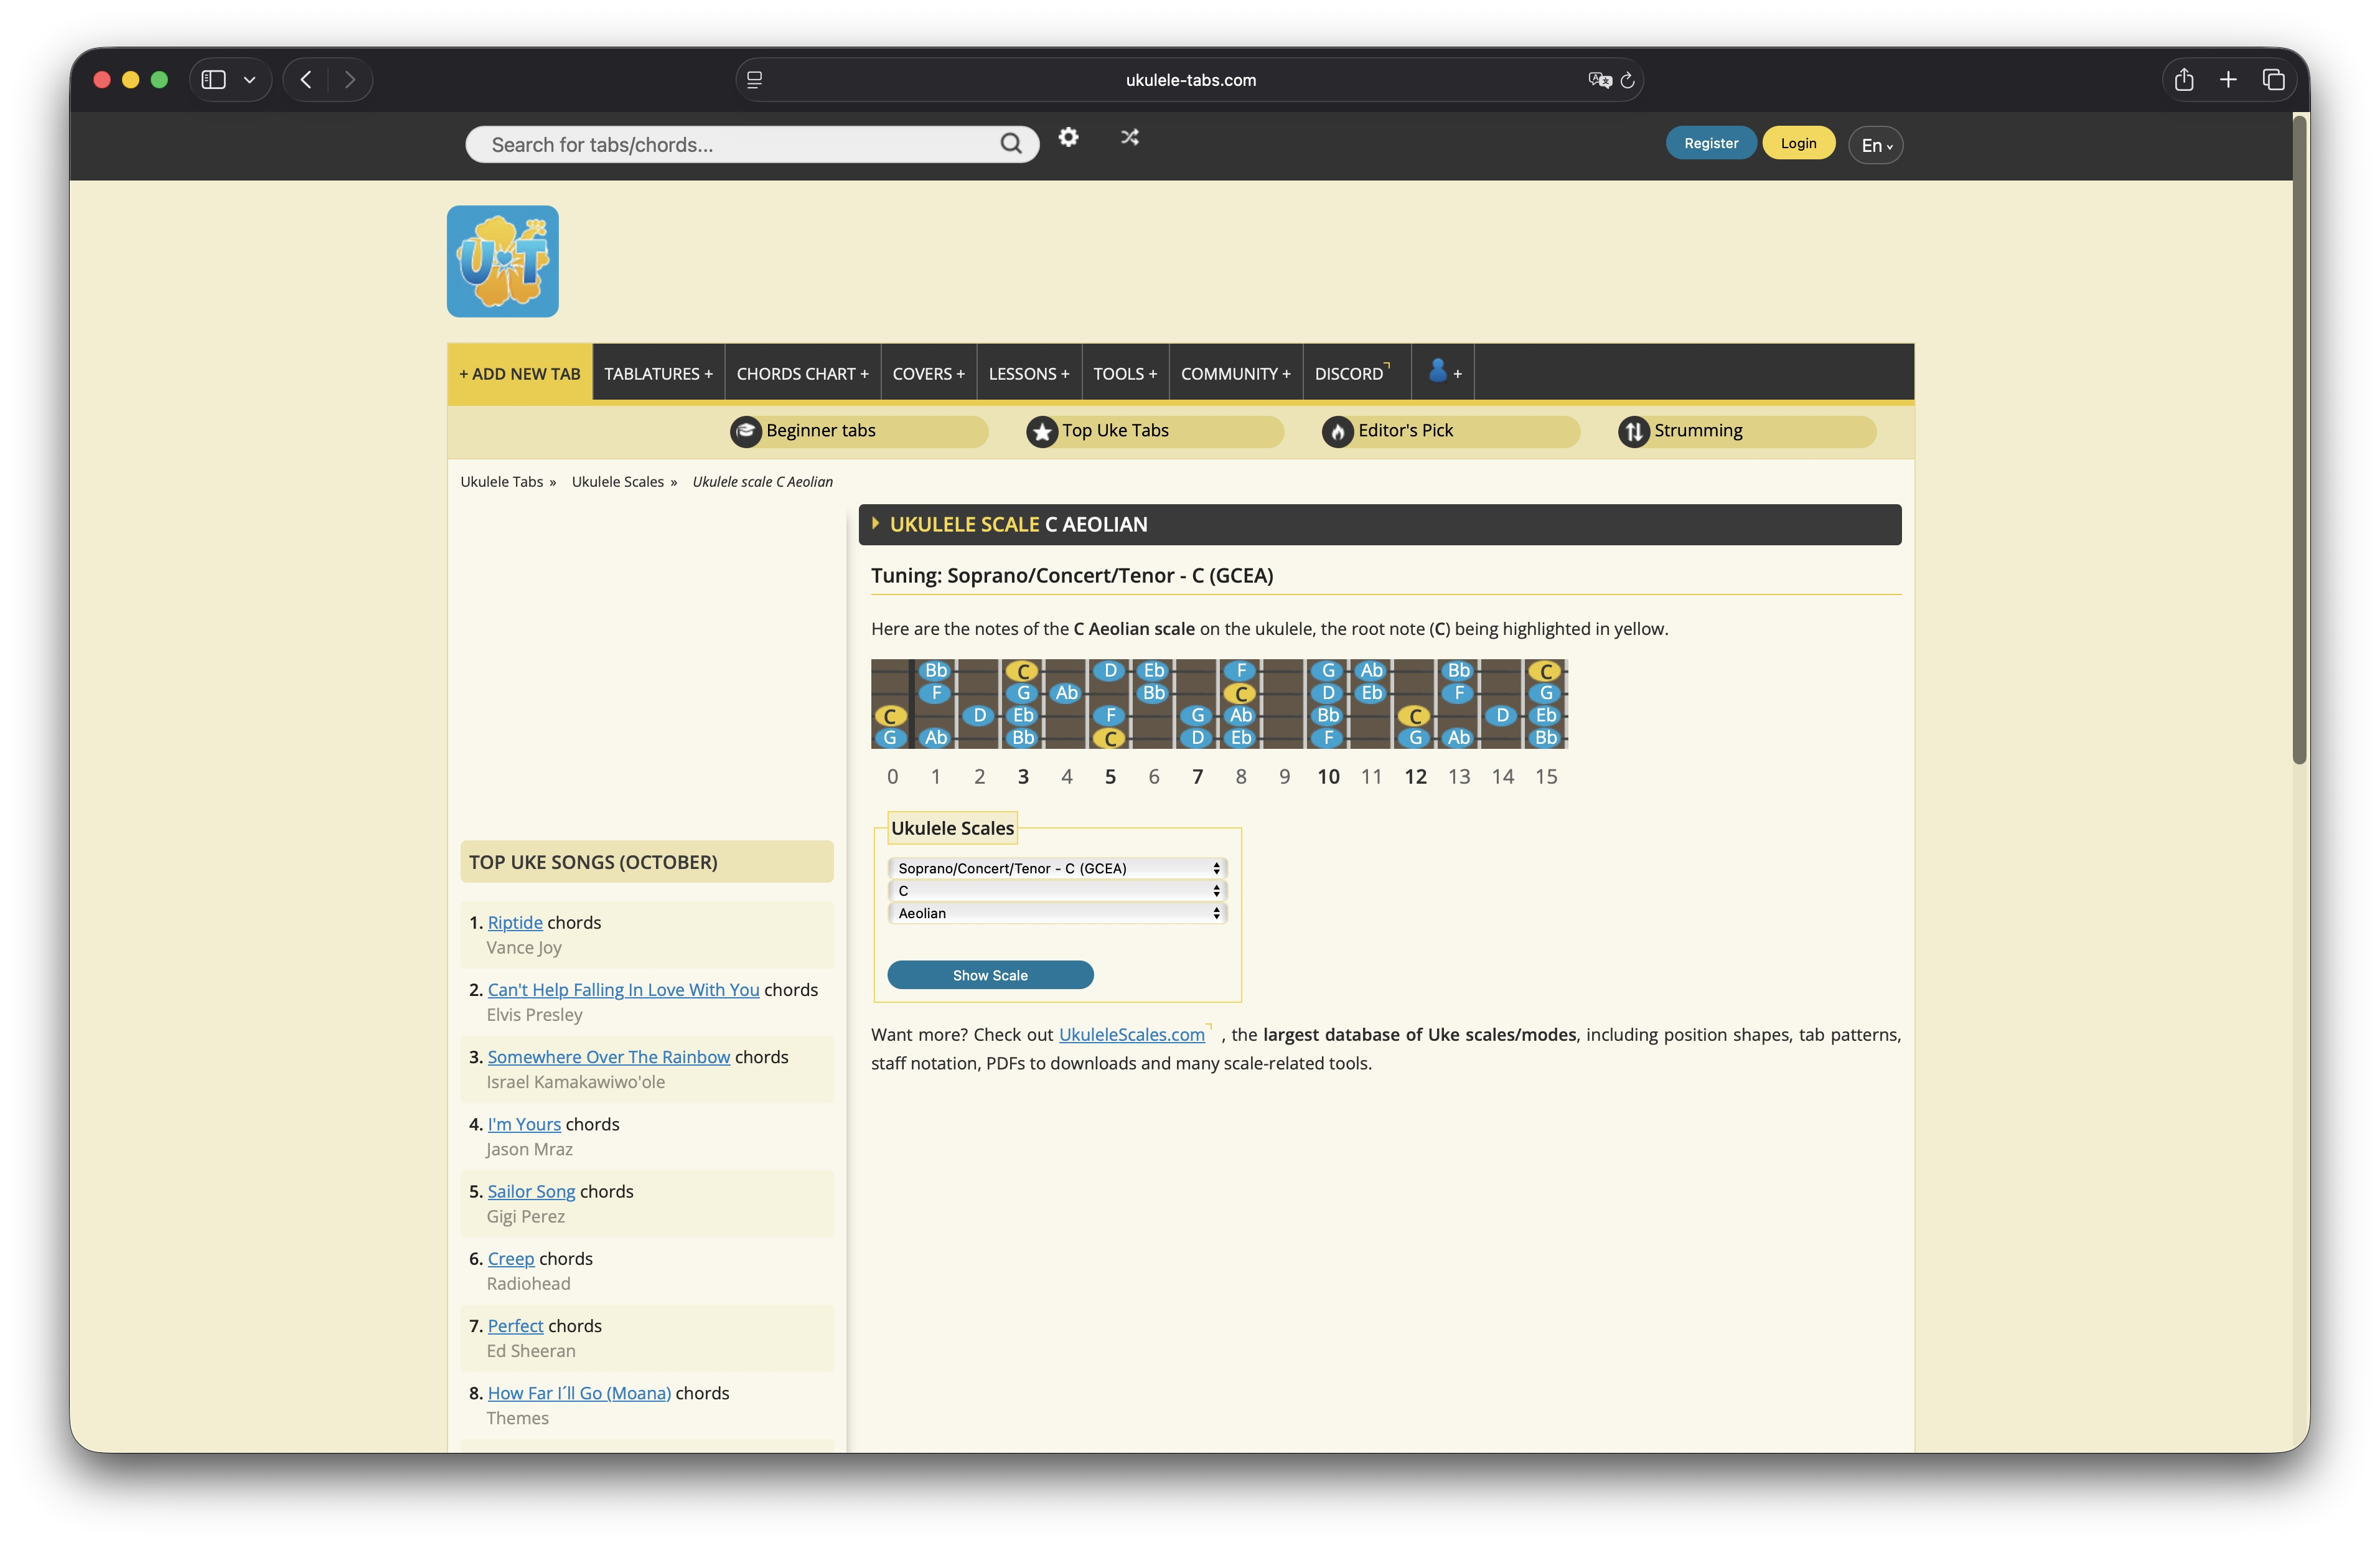
\includegraphics[width=\textwidth]{Ilustraciones/estado/ukuleletabs_escala.jpeg}
        \caption{Página de escalas de Ukulele Tabs~\cite{ukuleletabs_escala}}\label{fig:ukuleletabs_escalas}
    \end{subfigure}

    % caption general
    \caption{Páginas informativas de Ukulele Tabs}\label{fig:ukuleletabs_guias}
\end{figure}

En conclusión, Ukulele Tabs es una aplicación web sencilla y eficaz, con una comunidad activa que contribuye a la verificación del contenido. Aunque no posee un gran número de herramientas y utilidades, sobre todo interactivas, ofrece lo mínimo indispensable para introducirse y practicar con el ukelele. Además, la aplicación se monetiza a través de anuncios publicitarios, lo que permite el acceso gratuito a sus usuarios, poniendo a su disposición la mayoría de sus funcionalidades sin necesidad de registro (veáse Tabla~\ref{tab:ukuleletabs_funcionalidades_usuario}).

\begin{table}[H]
    \centering
    \scriptsize
    \begin{minipage}[t]{0.4\textwidth}
        \centering
        \caption{Utilidades presentes en publicaciones de Ukulele Tabs}\label{tab:ukuleletabs_utilidades_canciones}
        \begin{tabular}{l c}
            \hline
            \textbf{Utilidad} & \textbf{Existe} \\
            \hline
            Transportador & \ding{51} \\
            Lista de acordes & \ding{51} \\
            Autodesplazamiento & \ding{51} \\
            Impresión/Descarga & \ding{51} \\
            Cambio de notación &  \\
            Cambio de instrumento &  \\
            Guardar canción & \ding{51} \\
            Guía de rasgueos & \ding{51} \\
            \hline
        \end{tabular}
    \end{minipage}
    \hfill
    \begin{minipage}[t]{0.56\textwidth}
        \centering
        \caption{Funcionalidades disponibles según el rol del usuario de Ukulele Tabs}\label{tab:ukuleletabs_funcionalidades_usuario}\hfill
        \begin{tabular}{p{0.55\textwidth} c c }
            \hline
            \multirow{2}{*}{\textbf{Funcionalidad}} & \multicolumn{2}{c}{\textbf{Rol Usuario}} \\
             & Visitante & Registrado \\
            \hline
            Biblioteca de canciones & \ding{51} & \ding{51} \\
            Creación y edición de publicaciones &  & \ding{51}  \\
            Utilidades de publicaciones & \ding{51} & \ding{51} \\
            Puntuar publicaciones &  & \ding{51}  \\
            Comentar publicaciones &  & \ding{51}  \\
            Solicitar nuevas canciones &  & \ding{51}  \\
            Cursos y guías & \ding{51} & \ding{51} \\
            Afinador & \ding{51} & \ding{51}  \\
            Calculadora de escalas y notas & \ding{51} & \ding{51}  \\
            Diccionario de acordes & \ding{51} & \ding{51}  \\
            \hline
        \end{tabular}
    \end{minipage}
\end{table}
\subsection{UkuTabs}

UkuTabs\cite{ukuleletabs_home} es una aplicación web diseñada principalmente para el ukelele, aunque también ofrece soporte para otros instrumentos como la guitarra y el mandolín. Entre las páginas que componen la aplicacion destacamos las relacionadas con canciones, herramientas y las informativas.

En primer lugar, con respecto a las \textbf{páginas relacionadas con canciones}, podemos encontrar:

\begin{itemize}
    \item \textbf{Biblioteca de canciones} (véase Figura~\ref{fig:ukutabs_home}), con la posibilidad de realizar búsquedas avanzadas por género, artista, popularidad, dificultad, listas (navideñas, infántiles\ldots) o tipo (acordes, tablaturas o ambas).
    \item \textbf{Canciones} (véase Figura~\ref{fig:ukutabs_somewhereovertherainbow}), que contienen la letra, acordes y utilidades~(véase Tabla \ref{tab:ukutabs_utilidades_canciones}) para la práctica de las mismas.
    \item \textbf{Solicitudes} de nuevas canciones.
\end{itemize}

En segundo lugar, en cuanto a las \textbf{páginas informativas y herramientas}, podemos encontrar:
\begin{itemize}
    \item \textbf{Guías} (véase Figura~\ref{fig:ukutabs_guias}), con un listado de lecciones que abarcan todos los aspectos necesarios para introducirse al ukelele.
    \item \textbf{Diccionario de acordes} (véase Figura~\ref{fig:ukutabs_acordes}), que permite realizar búsquedas de acordes con la posibilidad de ser visualizada a través de un diagrama o en una simulación del mástil del instrumento.
    \item \textbf{Calculadora de escalas o notas}, que al introducir una nota muestra los resultados en una simulación del mástil del instrumento
    \item \textbf{Afinador de instrumento interactivo}, haciendo uso del micrófono integrado en el dispositivo.
\end{itemize}

\begin{figure}[H]
    \centering

    % Primera fila
    \begin{subfigure}[t]{0.48\textwidth}
        \centering
        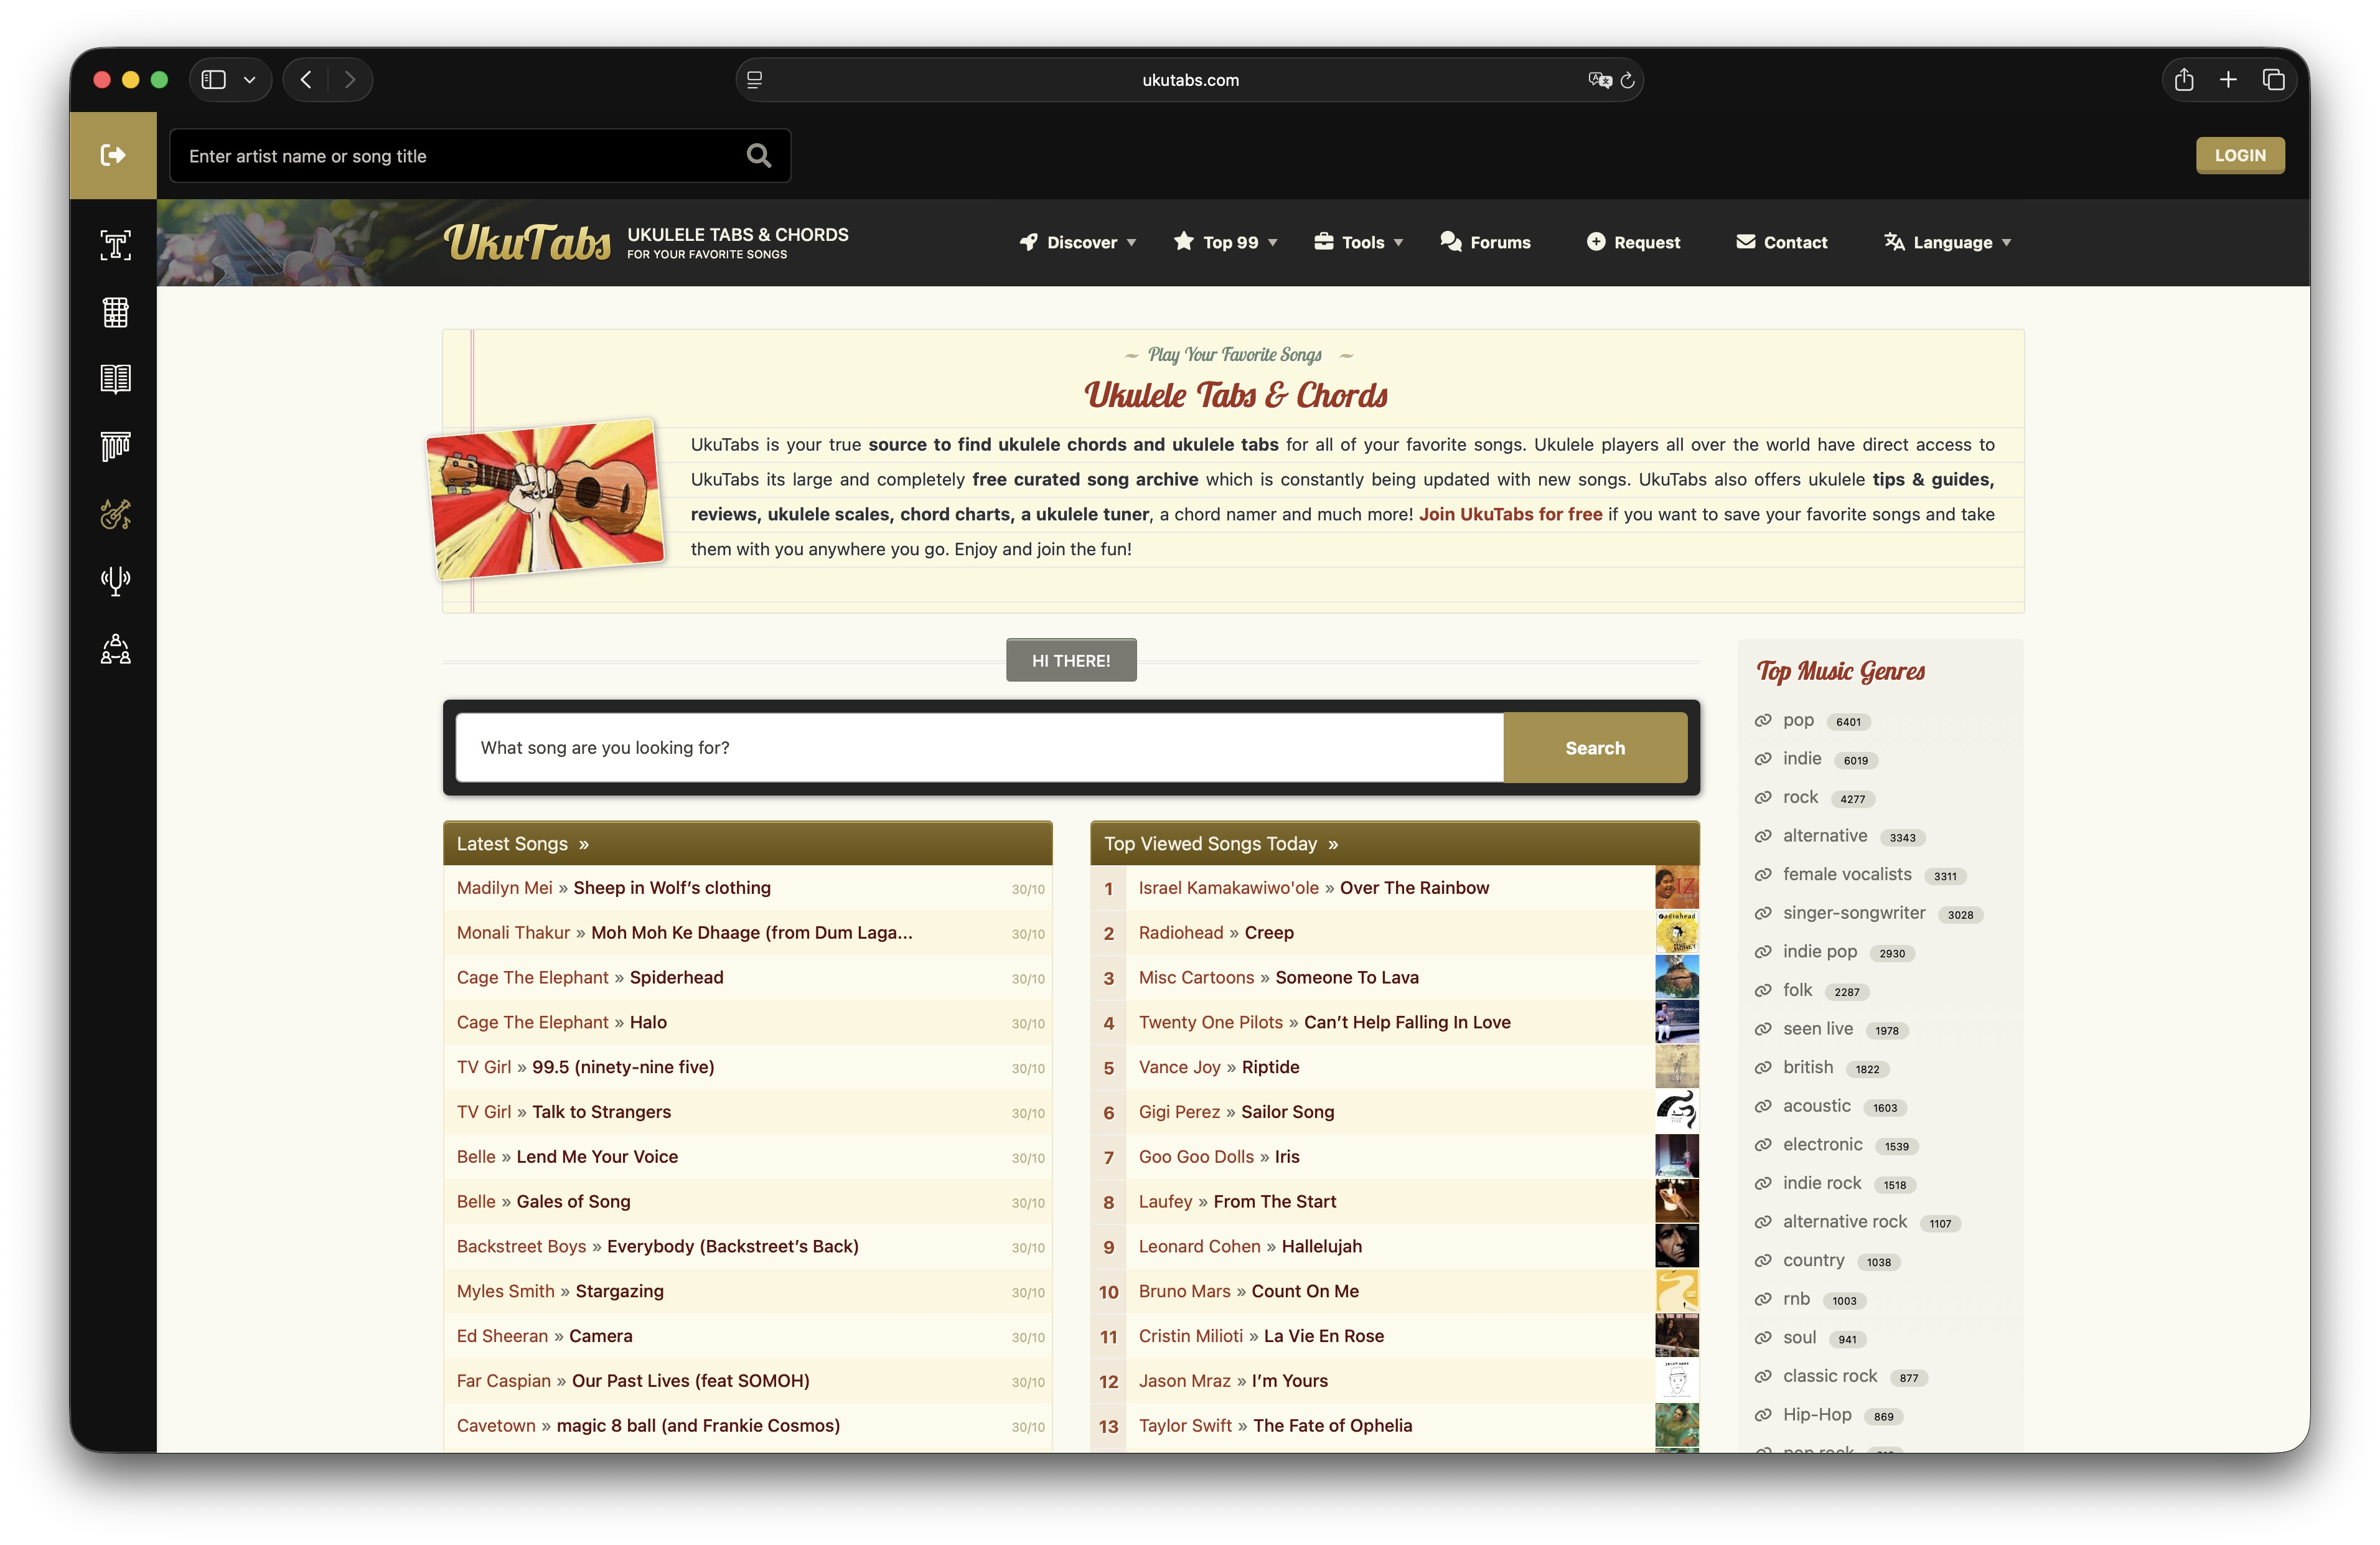
\includegraphics[width=\textwidth]{Ilustraciones/estado/ukutabs.jpeg}
        \caption{Página principal de UkuTabs~\cite{ukutabs_home}}
        \label{fig:ukutabs_home}
    \end{subfigure}
    \hfill
    \begin{subfigure}[t]{0.48\textwidth}
        \centering
        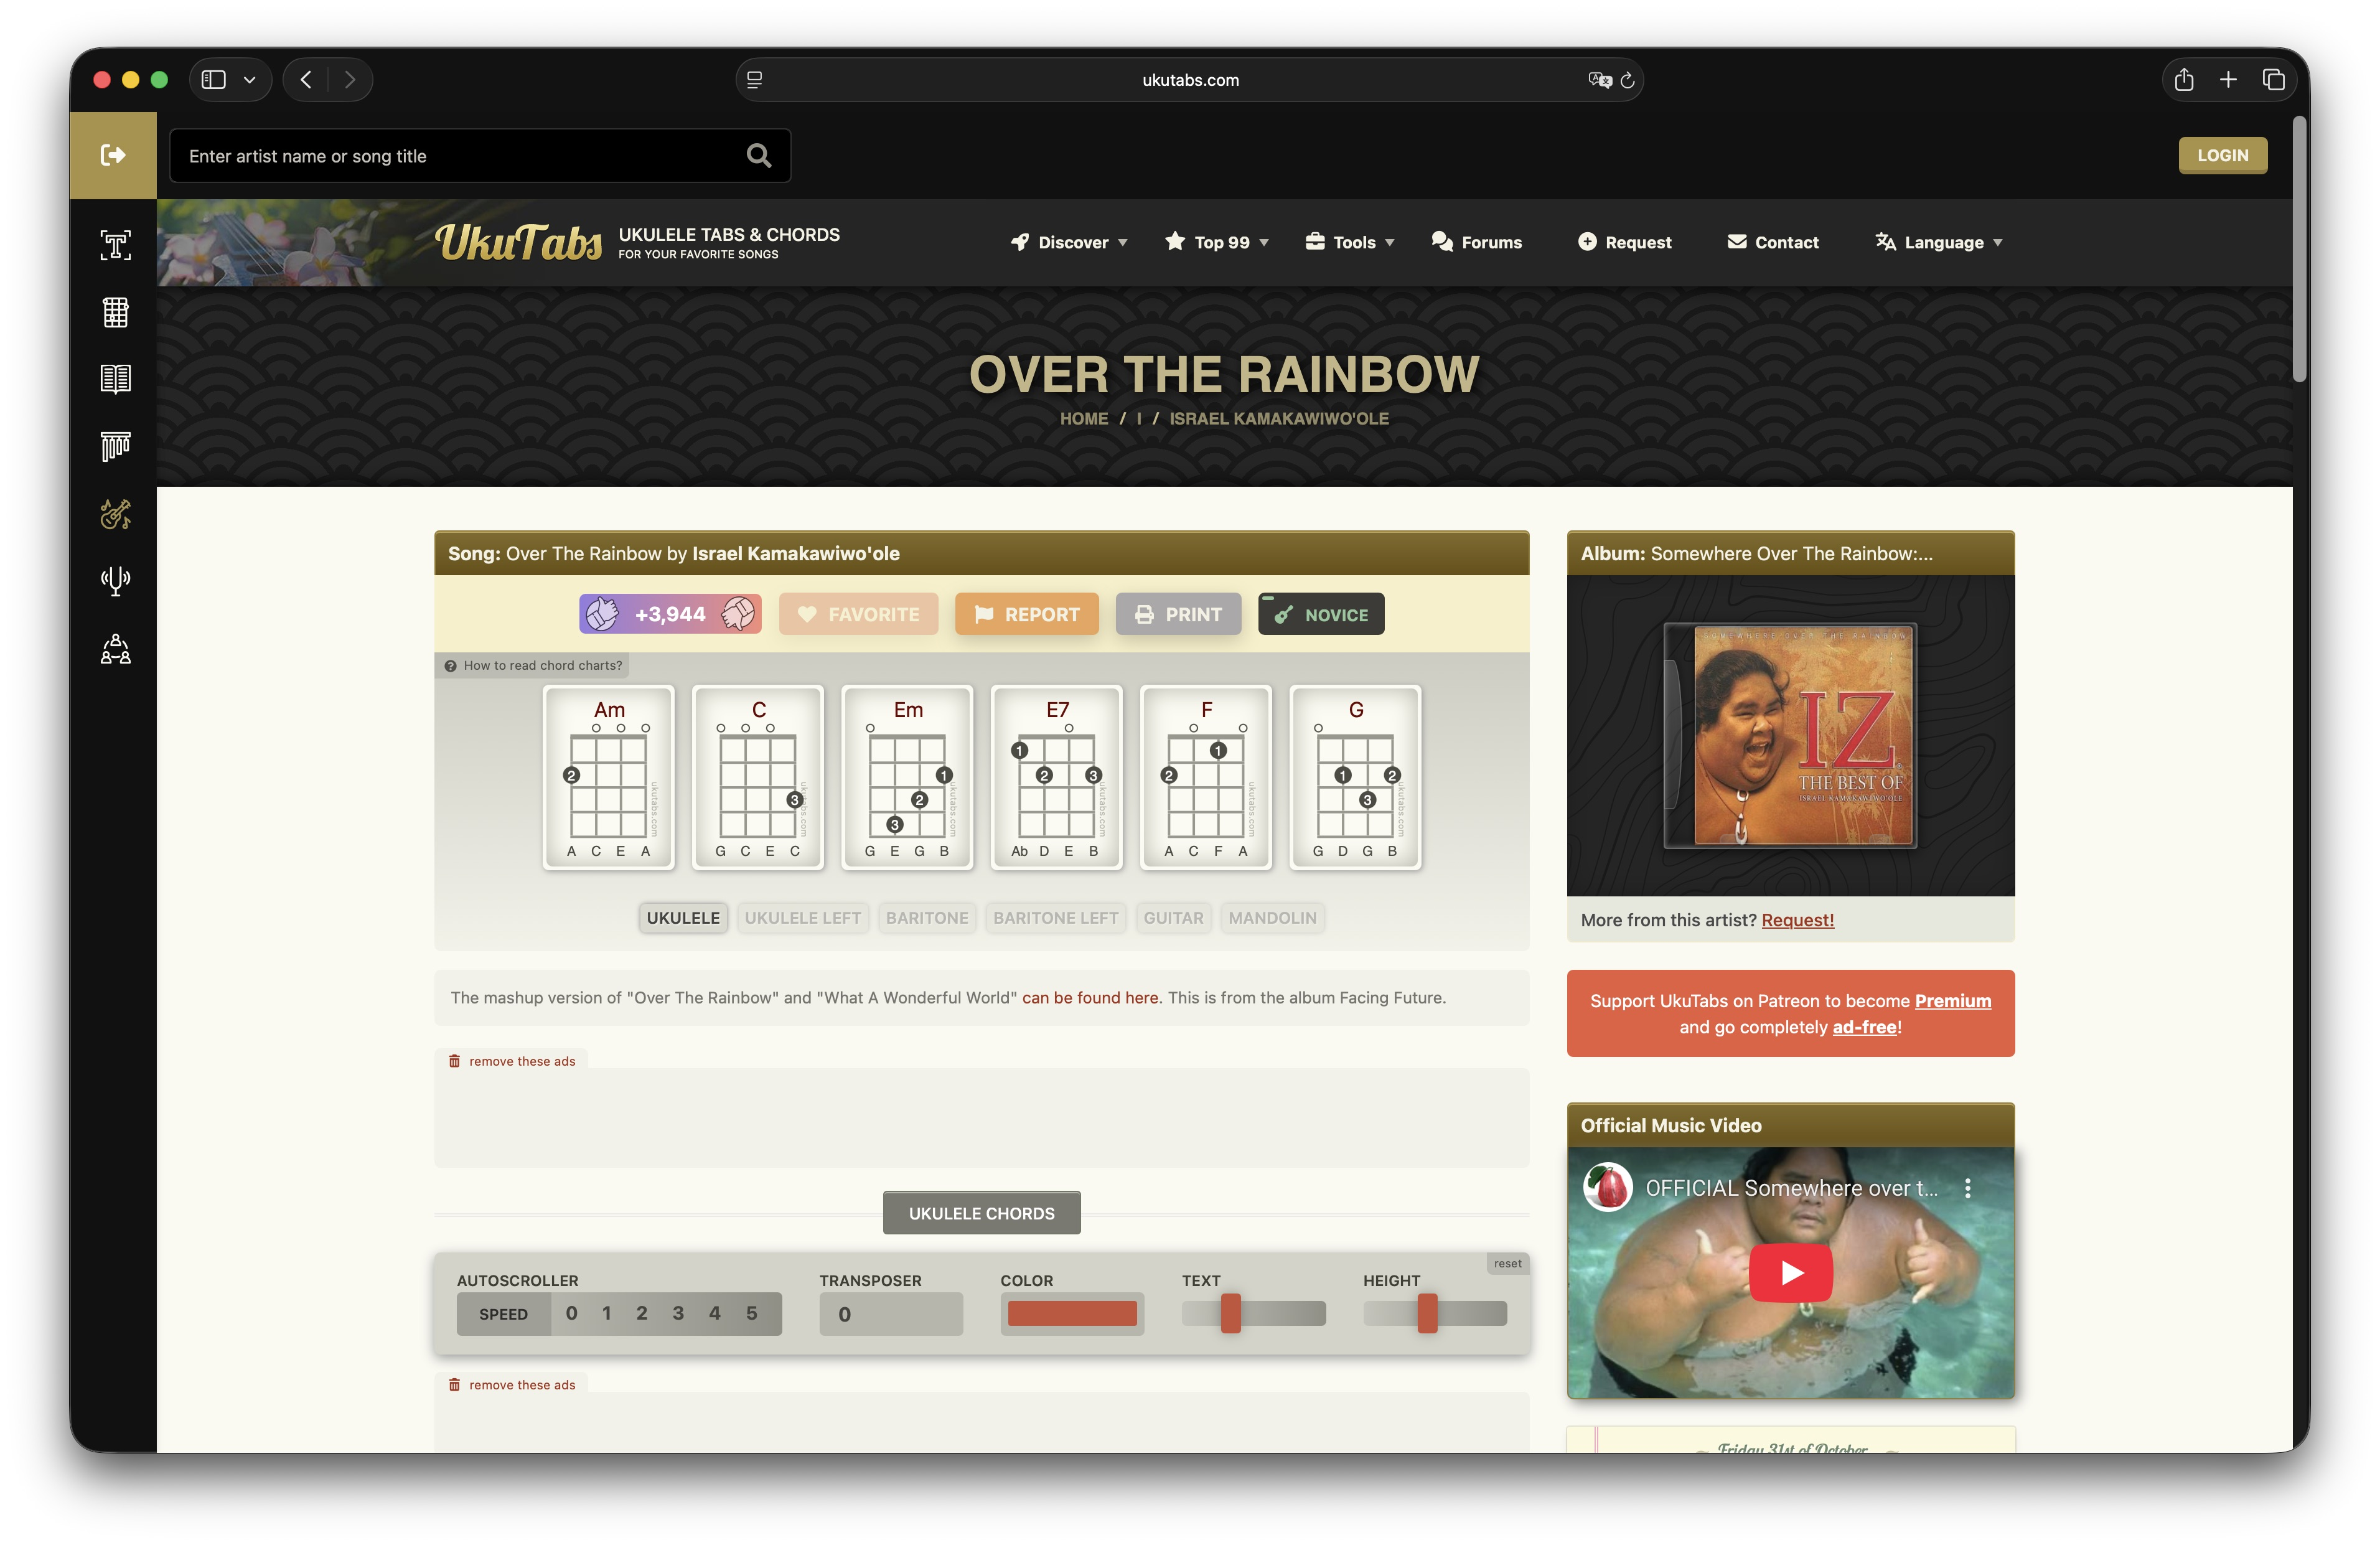
\includegraphics[width=\textwidth]{Ilustraciones/estado/ukutabs_somewhereovertherainbow.jpeg}
        \caption{Acordes y letra de \emph{Somewhere over the rainbow}~\cite{ukutabs_somewhereovertherainbow} para ukelele en UkuTabs}
        \label{fig:ukutabs_somewhereovertherainbow}
    \end{subfigure}

    \vspace{1em} % Espacio vertical entre filas

    % Segunda fila
    \begin{subfigure}[t]{0.48\textwidth}
        \centering
        \includegraphics[width=\textwidth]{Ilustraciones/estado/ukutabs_guías.jpeg}
        \caption{Página de guías de UkuTabs~\cite{ukutabs_guias}}
        \label{fig:ukutabs_guias}
    \end{subfigure}
    \hfill
    \begin{subfigure}[t]{0.48\textwidth}
        \centering
        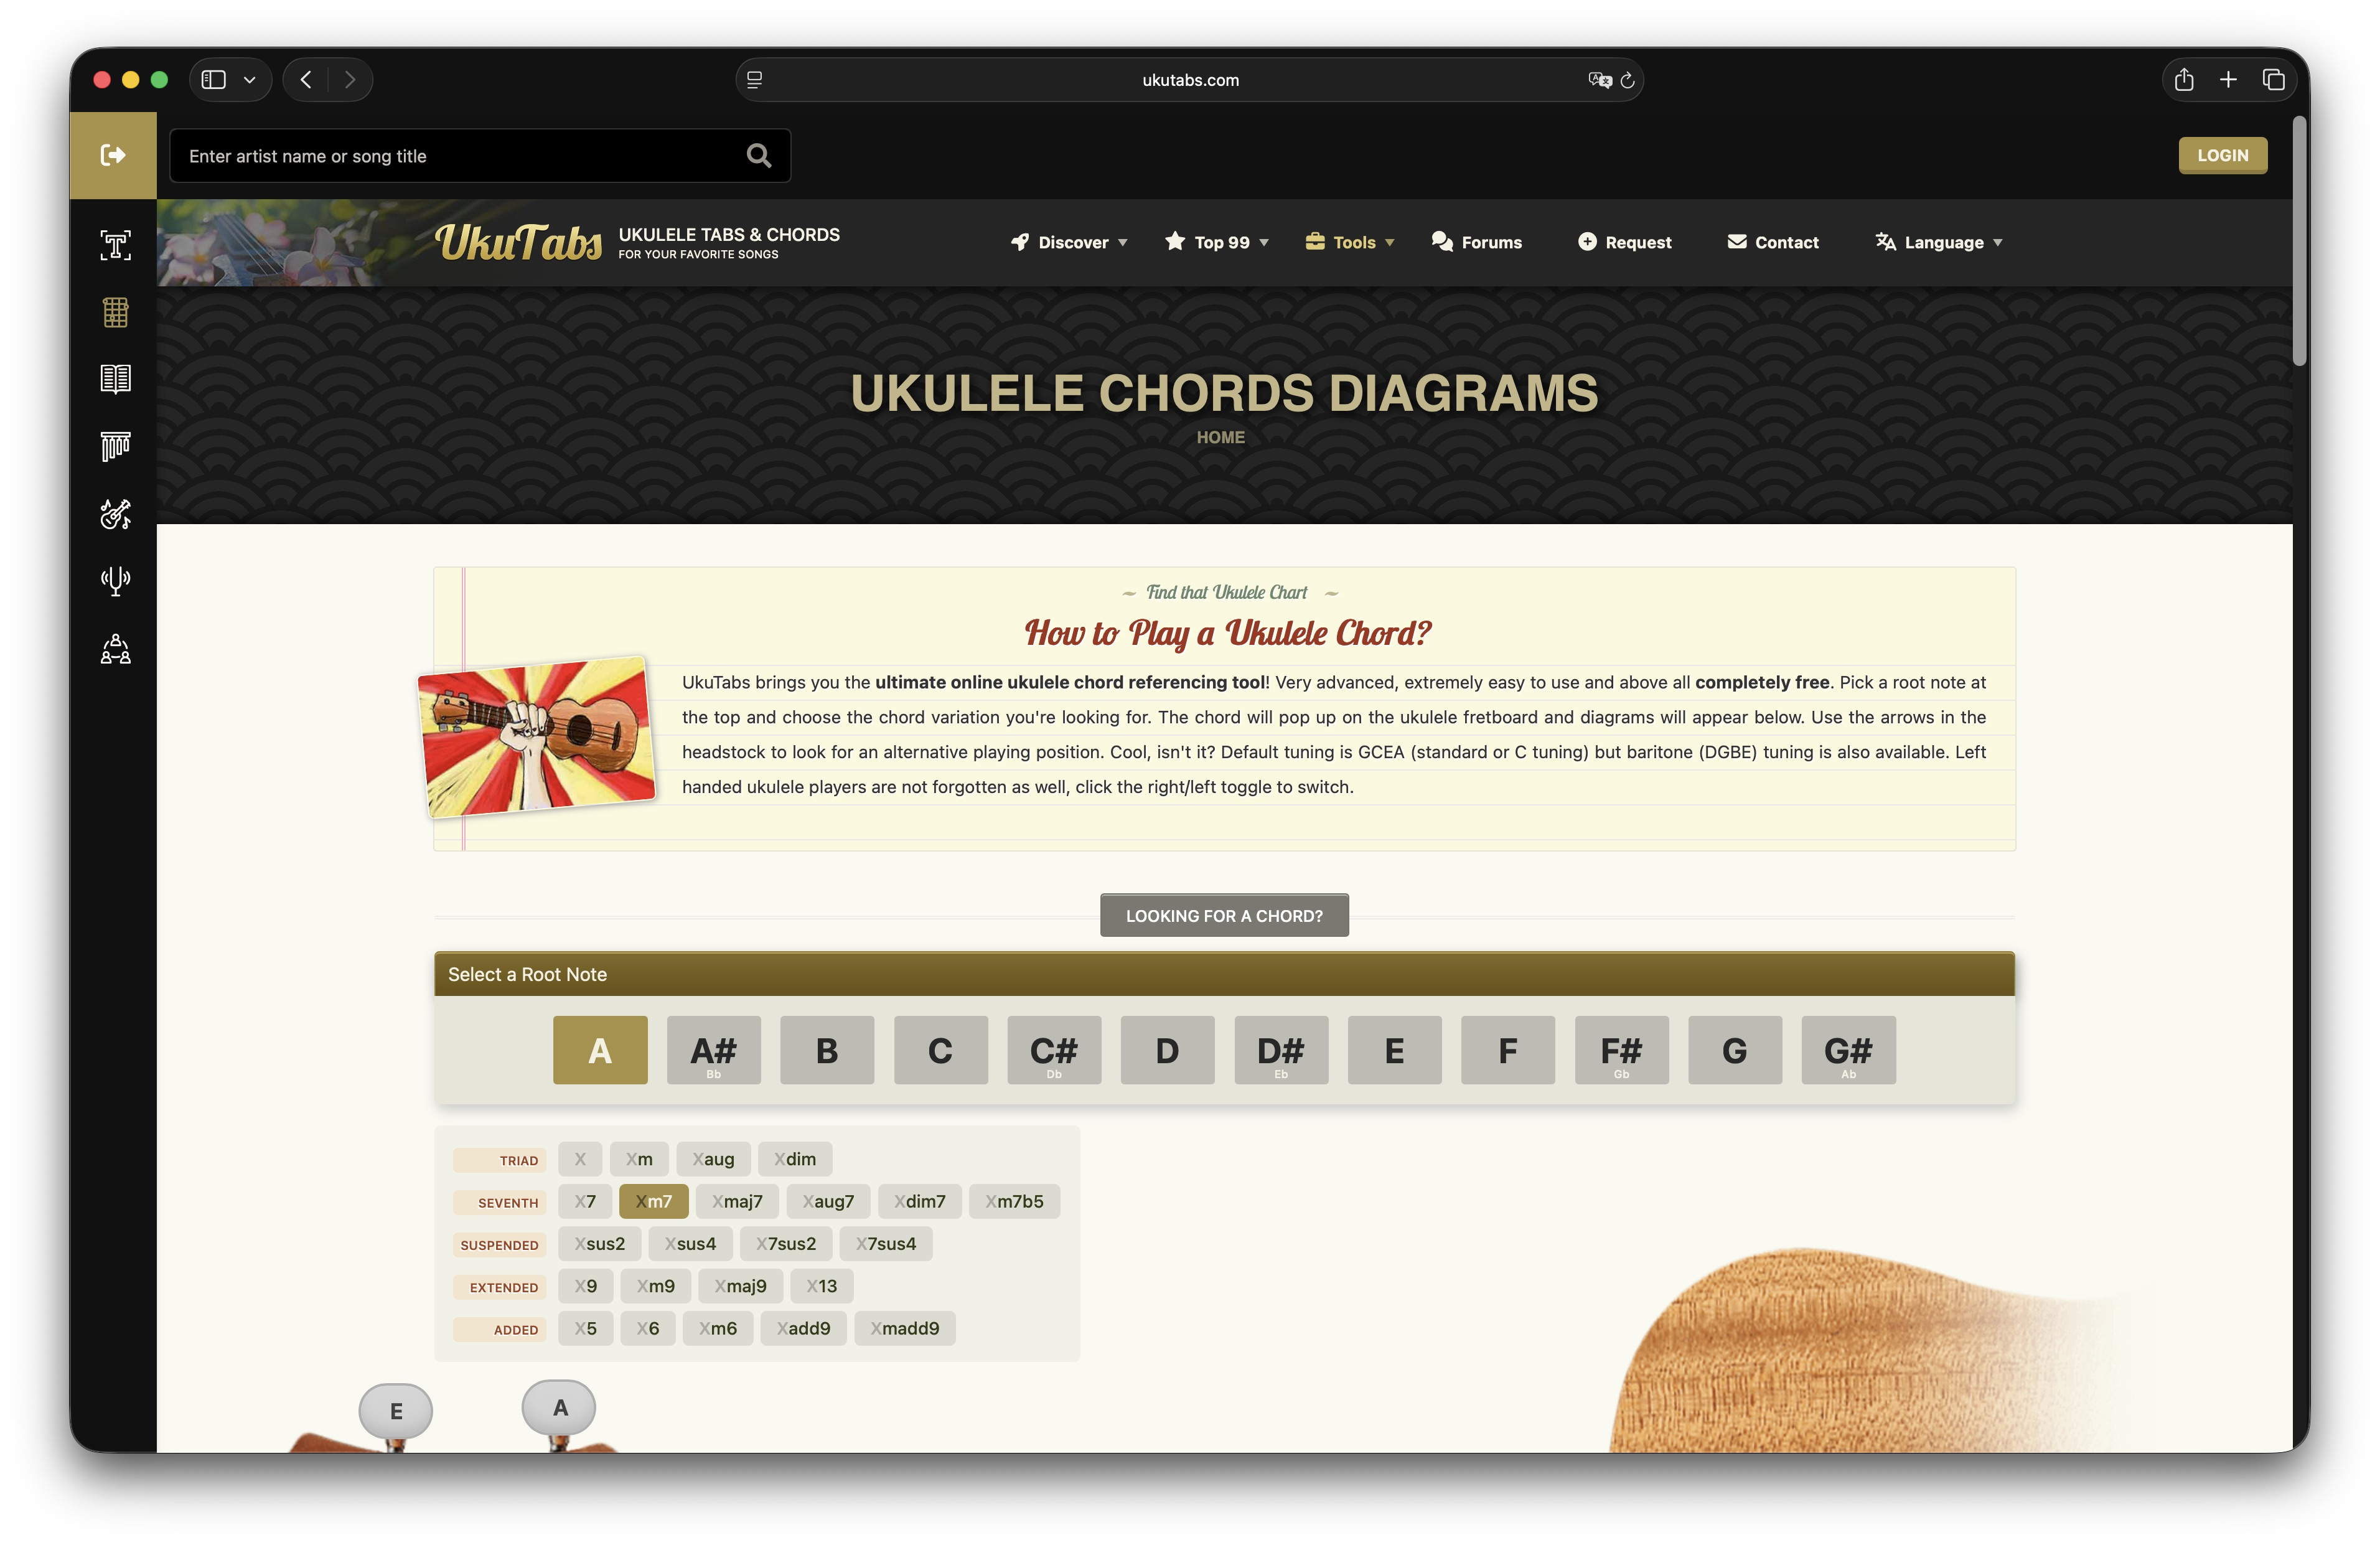
\includegraphics[width=\textwidth]{Ilustraciones/estado/ukutabs_acordes.jpeg}
        \caption{Página de acordes de UkuTabs~\cite{ukutabs_acordes}}
        \label{fig:ukutabs_acordes}
    \end{subfigure}

    \caption{Páginas de UkuTabs.}
    \label{fig:ukutabs_canciones}
\end{figure}

En conclusión, UkuTabs es una aplicación web muy cuidada, tanto en el nivel funcional como en el visual. Nos encontramos ante un producto que ofrece una experiencia de usuario completa y eficaz, con un gran número de herramientas interactivas y un sistema de verificación de contenido mediante administradores que garantiza la calidad de sus contenidos. Además, la aplicación se monetiza a través de anuncios, lo que permite el acceso gratuito a sus usuarios, poniendo a su disposición la mayoría de sus funcionalidades sin necesidad de registro (véase Tabla~\ref{tab:ukutabs_funcionalidades_usuario}).

\begin{table}[H]
    \scriptsize
    \begin{minipage}[t]{0.4\textwidth}
        \centering
        \caption{Utilidades presentes en publicaciones de UkuTabs}\label{tab:ukutabs_utilidades_canciones}
        \begin{tabular}{l c}
            \hline
            \textbf{Utilidad} & \textbf{Existe} \\
            \hline
            Transportador & \ding{51} \\
            Lista de acordes & \ding{51} \\
            Autodesplazamiento & \ding{51} \\
            Impresión/Descarga & \ding{51} \\
            Cambio de notación &  \\
            Cambio de instrumento & \ding{51} \\
            Guardar canción & \ding{51} \\
            Guía de rasgueos & \\
            \hline
        \end{tabular}
    \end{minipage}
    \hfill
    \begin{minipage}[t]{0.56\textwidth}
        \centering
        \caption{Funcionalidades disponibles según el rol del usuario de UkuTabs}\label{tab:ukutabs_funcionalidades_usuario}
        \begin{tabular}{l c c }
            \hline
            \multirow{2}{*}{\textbf{Funcionalidad}} & \multicolumn{2}{c}{\textbf{Rol Uusario}} \\
            & Visitante & Registrado \\
            \hline
            % --- Ejemplo de fila vacía (borra o completa) ---
            Biblioteca de canciones & \ding{51} & \ding{51} \\
            Creación y edición de publicaciones &  & \ding{51}  \\
            Utilidades de publicaciones & \ding{51} & \ding{51} \\
            Puntuar publicaciónes &  & \ding{51}  \\
            Comentar publicaciones &  & \ding{51}  \\
            Solicitar nuevas canciones & \ding{51}  & \ding{51}  \\
            Cursos y guías & \ding{51} & \ding{51} \\
            Afinador & \ding{51} & \ding{51}  \\
            Calculadora de escalas y notas & \ding{51} & \ding{51}  \\
            Diccionario de acordes & \ding{51} & \ding{51}  \\
            % ------------------------------------------------
            \hline
        \end{tabular}
    \end{minipage}
    
\end{table}
\subsection{Ultimate Guitar}
UltimateGuitar\cite{ultimateguitar_home} es una aplicación web diseñada específicamente para guitarra, aunque tambien ofrece soporte para otros instrumentos como el ukelele, el bajo y el piano. Aunque podemos encontrar páginas dedicadas a artículos, libros y un foro, destacamos las relacionadas con canciones y los cursos.

En primer lugar, con respecto a las \textbf{páginas relacionadas con canciones}, podemos encontrar:
\begin{itemize}
    \item \textbf{Biblioteca de canciones} (véase Figura~\ref{fig:ultimateguitar_home}), con la posibilidad de realizar búsquedas avanzadas por género, artista, popularidad y tipo (acordes, tablatura, instrumento\dots).
    \item \textbf{Canciones} (véase Figura~\ref{fig:ultimateguitar_somewhereovertherainbow}) que contienen la letra, acordes y utilidades~(véase Tabla~\ref{tab:ultimateguitar_utilidades_canciones}) para la práctica de las mismas.
\end{itemize}


En segundo lugar, en cuanto a los \textbf{cursos} (véase Figura~\ref{fig:ultimateguitar_courses}), Ultimate Guitar ofrece un catálogo de cursos para usuarios de distintos niveles. Estos incluyen vídeos, ejercicios interactivos y material descargable.

\begin{figure}[H]
    \centering
    % Primera fila
    \begin{subfigure}[t]{0.48\textwidth}
         \centering
        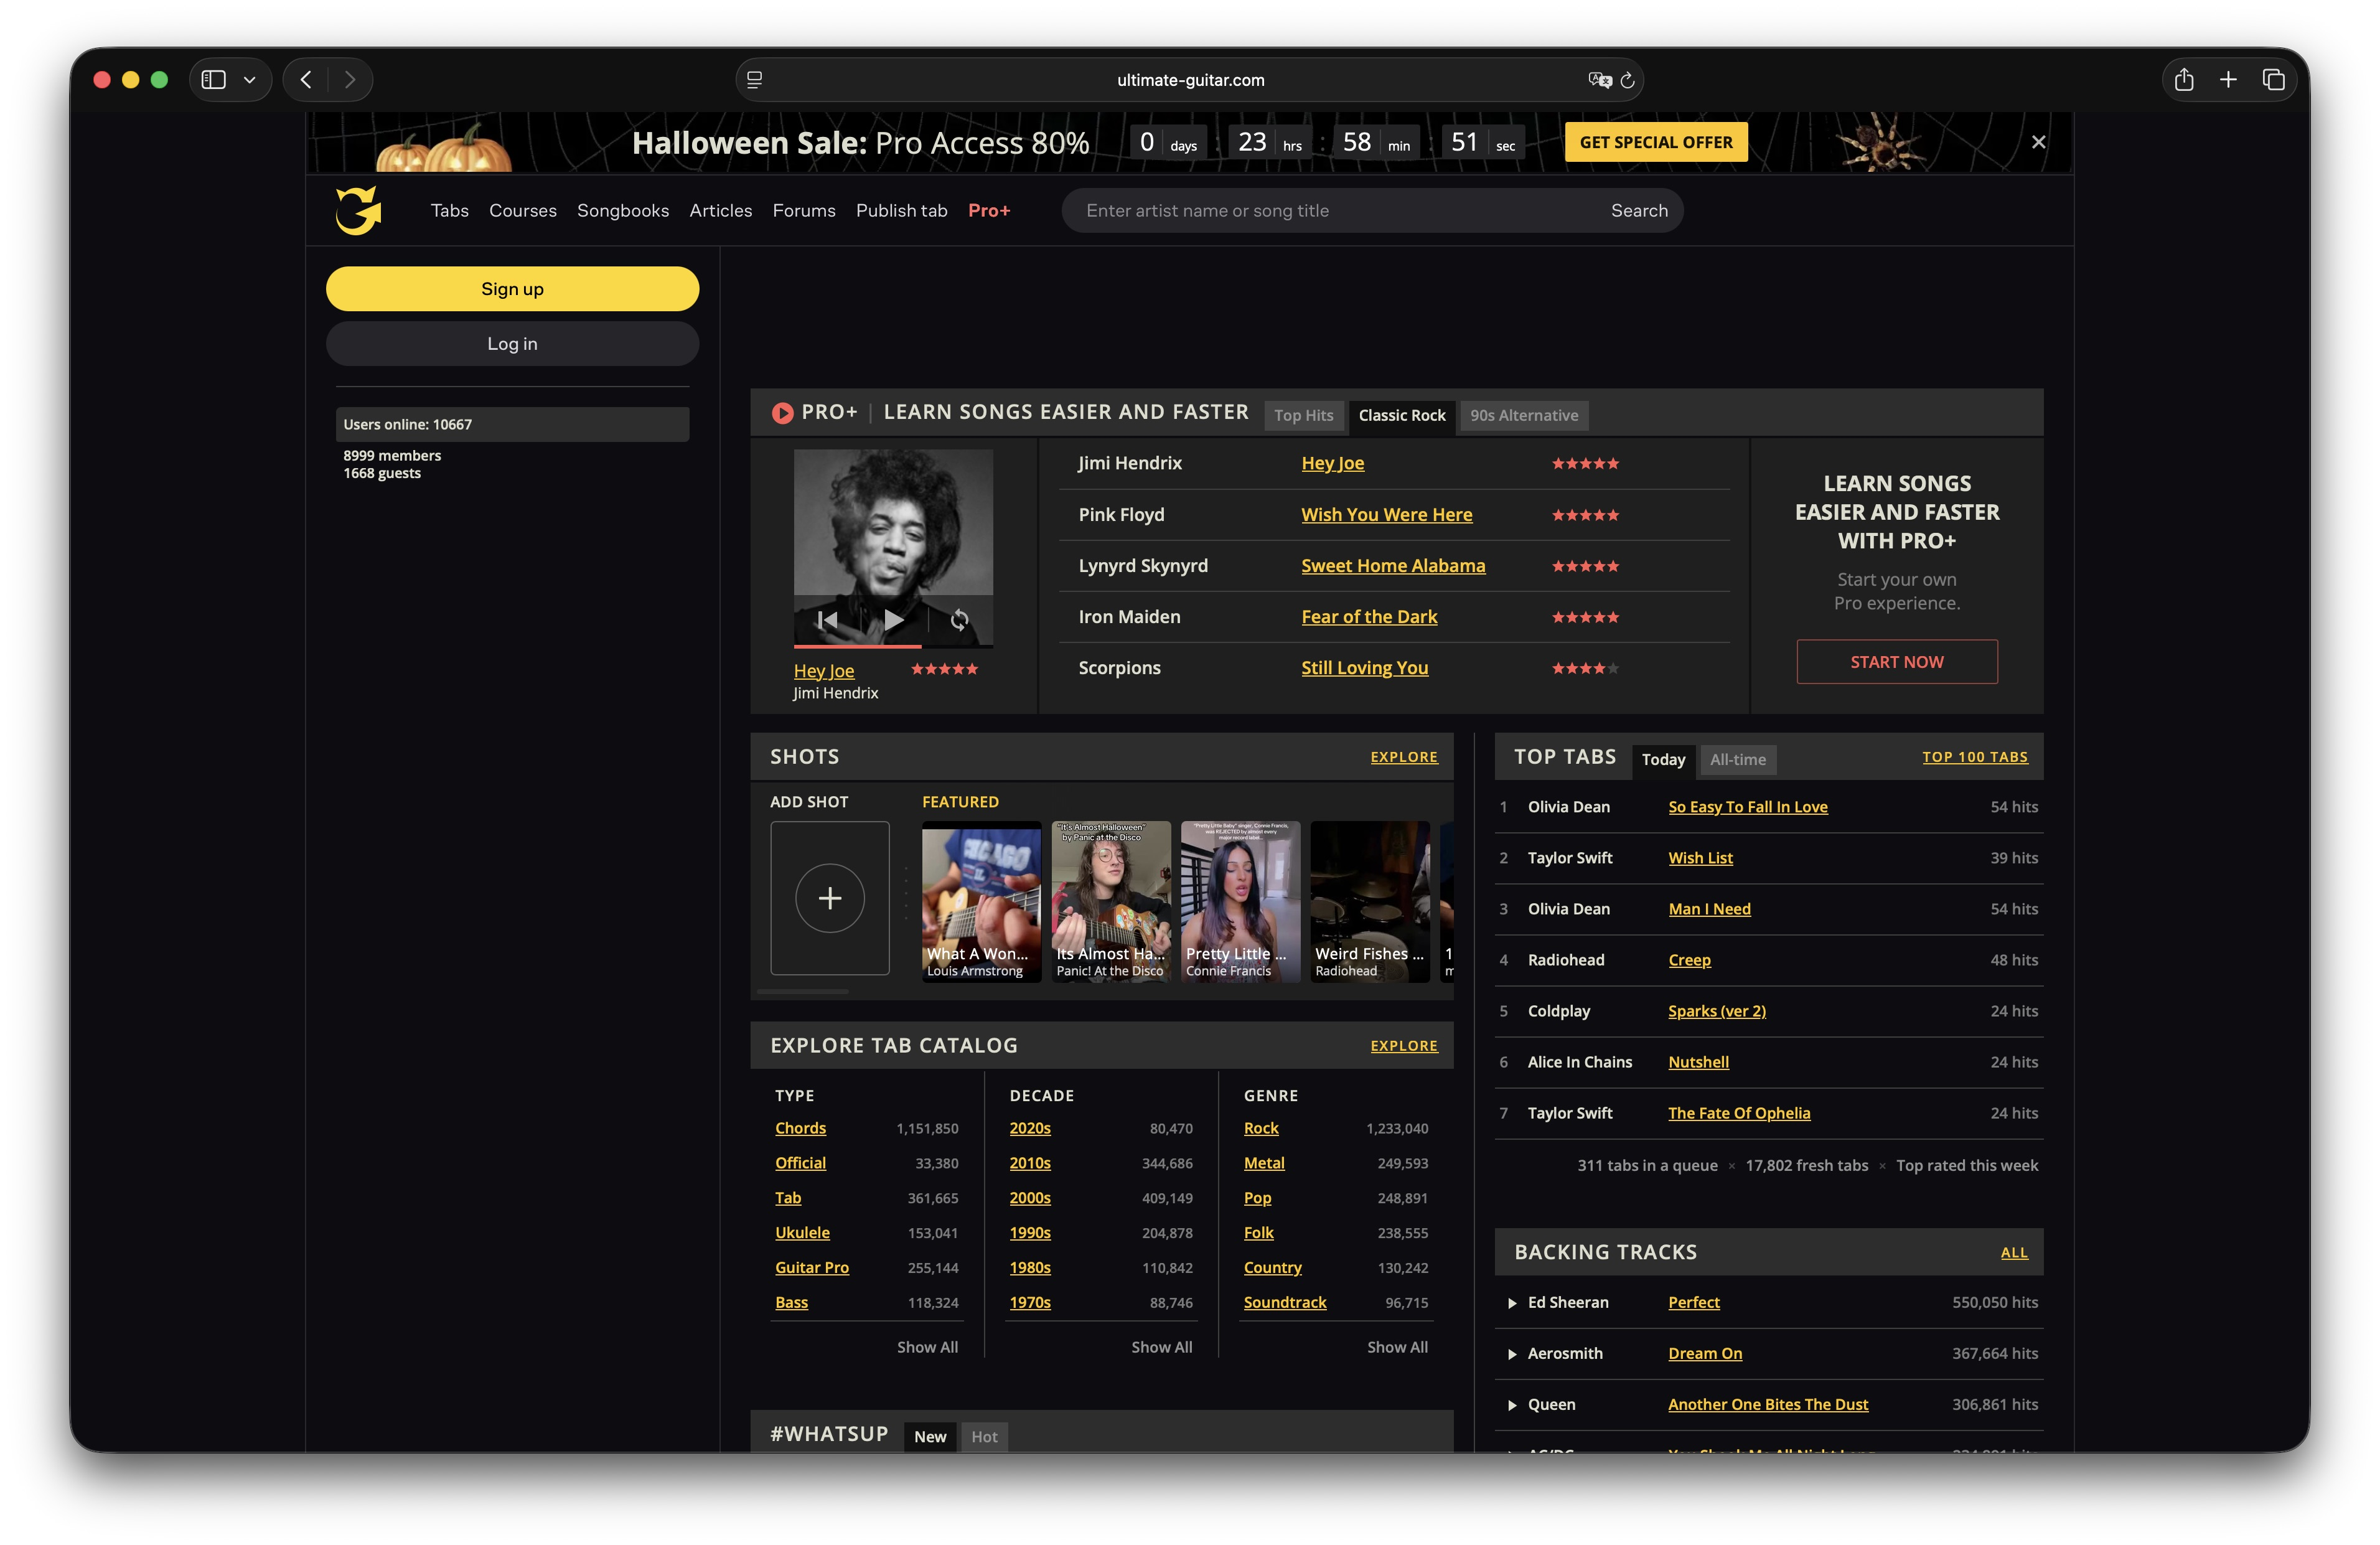
\includegraphics[width=\textwidth]{Ilustraciones/estado/ultimateguitar.jpeg}
        \caption{Página principal de Ultimate Guitar~\cite{ultimateguitar_home}}\label{fig:ultimateguitar_home}
    \end{subfigure}
    \hfill
    \begin{subfigure}[t]{0.48\textwidth}
        \centering
        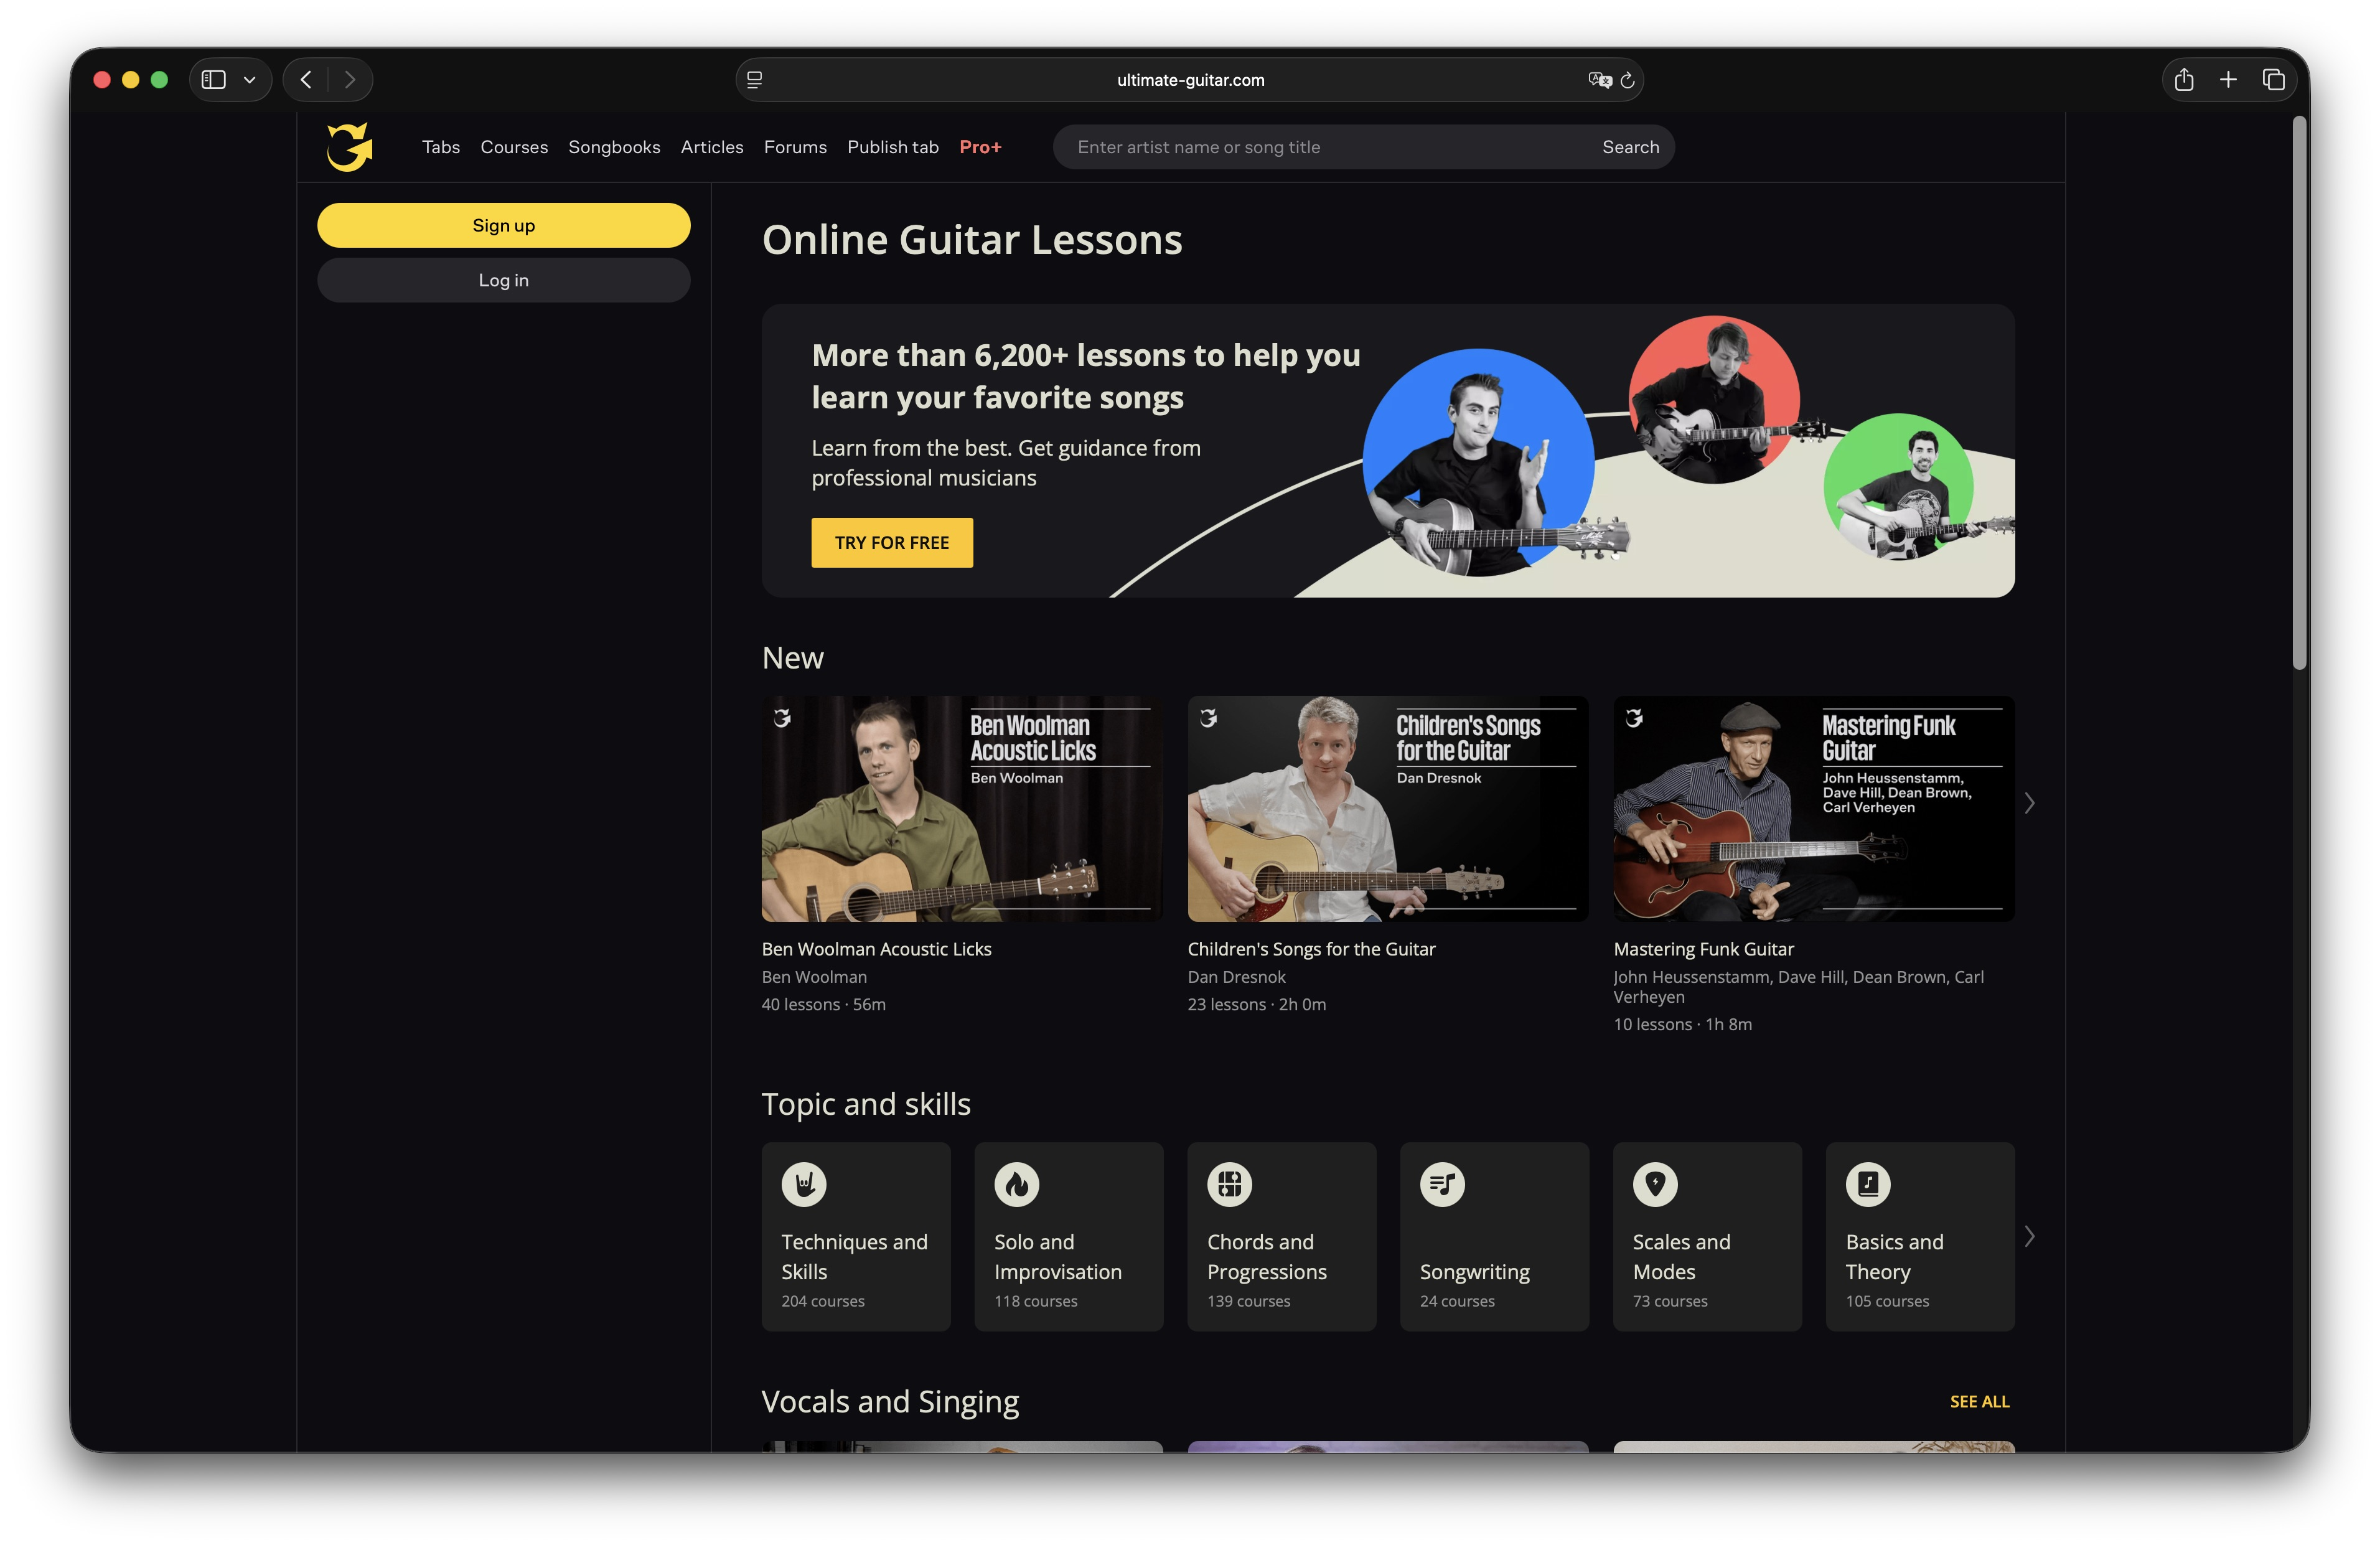
\includegraphics[width=\textwidth]{Ilustraciones/estado/ultimateguitar_courses.jpeg}
        \caption{Página de cursos de Ultimate Guitar~\cite{ultimateguitar_courses}}
        \label{fig:ultimateguitar_courses}
    \end{subfigure}
    \vspace{1em} % Espacio vertical entre filas

    % Segunda fila
    \begin{subfigure}[t]{\textwidth}
        \centering
        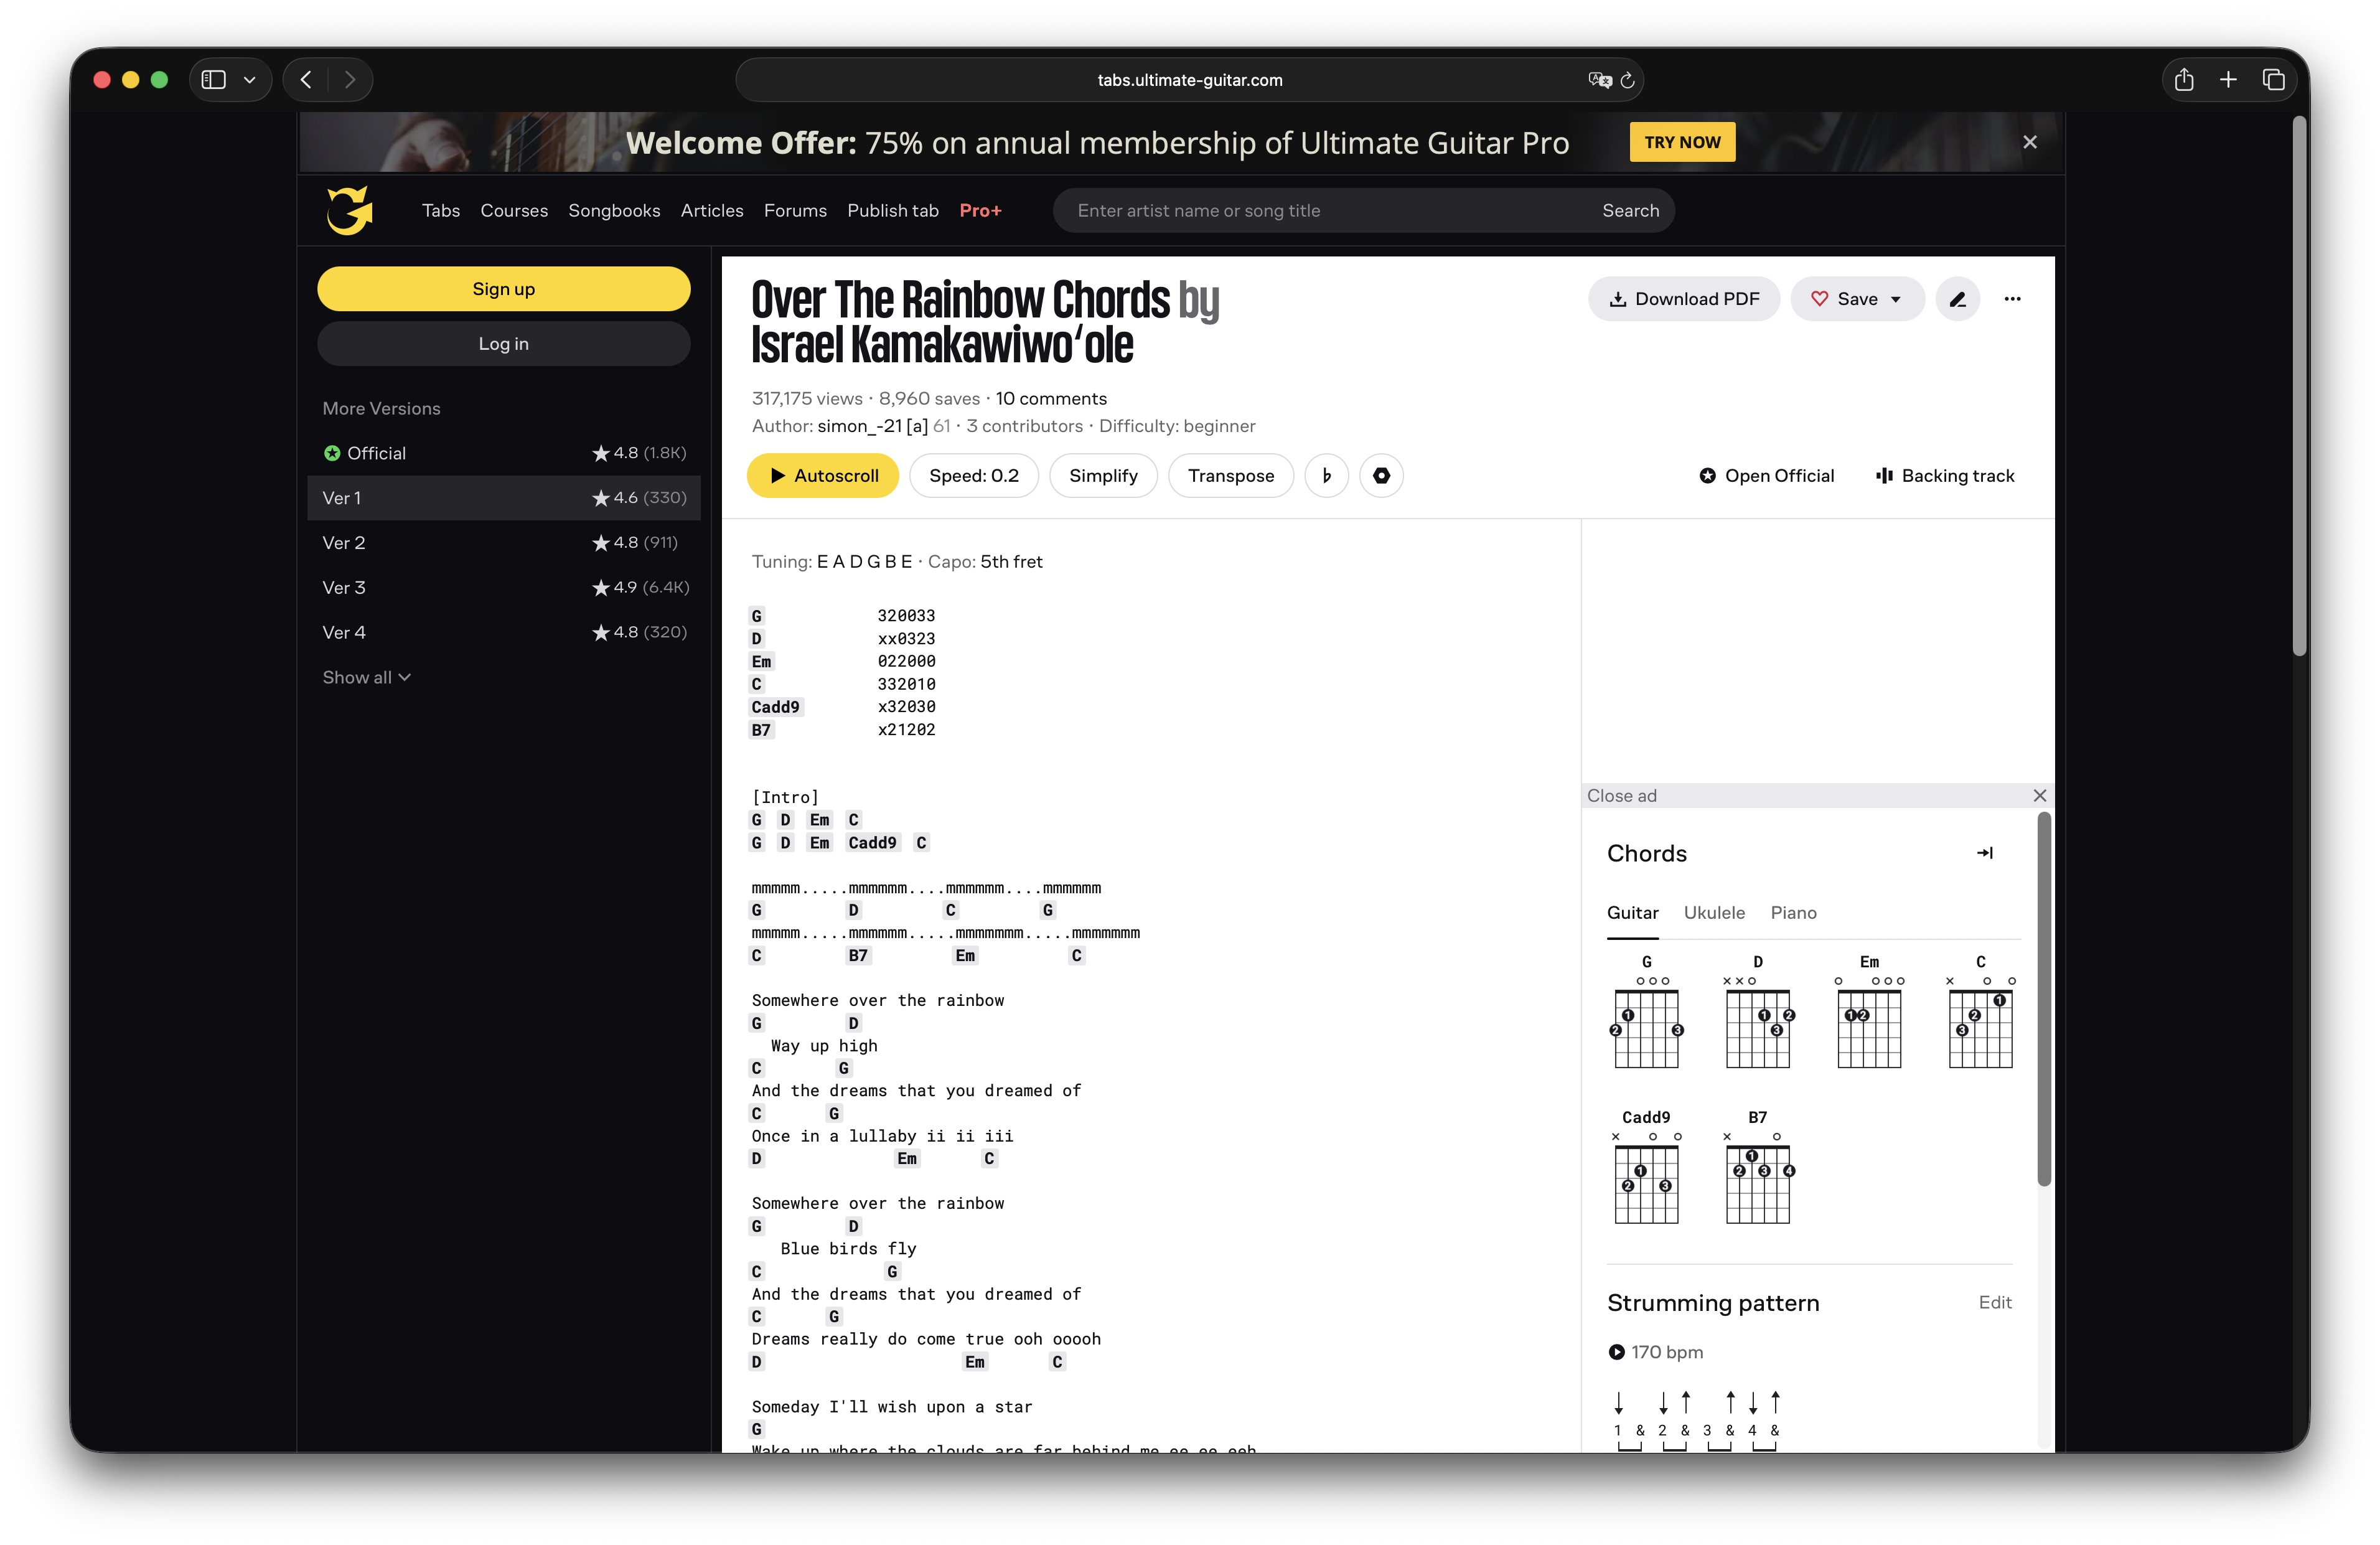
\includegraphics[width=0.8\textwidth]{Ilustraciones/estado/ultimateguitar_somewhereovertherainbow.jpeg}
        \caption{Acordes y letra de \emph{Somewhere over the rainbow}~\cite{ultimateguitar_somewhereovertherainbow} en Ultimate Guitar}
        \label{fig:ultimateguitar_somewhereovertherainbow}
    \end{subfigure}

    \caption{Páginas de Ultimate Guitar.}
    \label{fig:ultimateguitar_canciones}
\end{figure}

En conclusión, Ultimate Guitar es una aplicación web completa, ofreciendo una gran cantidad de utilidades, muchas de ellas interactivas. Su sistema de verificación a traves de la comunidad, permite además ampliar el catálogo de canciones disponibles, pudiendo encontrar varias versiones de una misma canción. No obstante, aunque gran parte de su contenido es accesible de forma gratuita, algunas funcionalidades avanzadas requieren una suscripción de pago. Para este análisis solo se tendrán en cuenta las funcionalidades que ofrezca en común con las otras alternativas seleccionadas (véase Tabla~\ref{tab:ultimateguitar_funcionalidades_usuario}).

\begin{table}[H]
    \scriptsize
    \begin{minipage}[t]{0.35\textwidth}
        \centering
        \caption{Utilidades presentes en publicaciones de Ultimate Guitar}\label{tab:ultimateguitar_utilidades_canciones}
        \begin{tabular}{l c}
            \hline
            \textbf{Utilidad} & \textbf{Existe} \\
            \hline
            Transportador & \ding{51} \\
            Lista de acordes & \ding{51} \\
            Autodesplazamiento & \ding{51} \\
            Impresión/Descarga & \ding{51} \\
            Cambio de notación &  \\
            Cambio de instrumento & \ding{51} \\
            Guardar canción & \ding{51} \\
            Guía de rasgueos & \ding{51} \\
            \hline
        \end{tabular}
    \end{minipage}
        \hfill
    \begin{minipage}[t]{0.61\textwidth}
        \centering
        \caption{Funcionalidades disponibles según el rol del usuario de Ultimate Guitar (Vis. Visitante, Reg. registrado y Sub. Suscrito)}\label{tab:ultimateguitar_funcionalidades_usuario}
        \begin{tabular}{l c c c }
            \hline
            \multirow{2}{*}{\textbf{Funcionalidad}} & \multicolumn{2}{c}{\textbf{Rol Usuario}} \\
            & Vis. & Reg. & Sub. \\
            \hline
            % --- Ejemplo de fila vacía (borra o completa) ---
            Biblioteca de canciones & \ding{51} & \ding{51} & \ding{51} \\
            Creación y edición de publicaciones &  & \ding{51} & \ding{51}  \\
            Utilidades de publicaciones & \ding{51} & \ding{51} & \ding{51} \\
            Puntuar publicaciónes &  & \ding{51} & \ding{51}  \\
            Comentar publicaciones &  & \ding{51} & \ding{51}  \\
            Solicitar nuevas canciones & & & \\
            Cursos y guías & & & \ding{51} \\
            Afinador & \ding{51} & \ding{51} & \ding{51}  \\
            Calculadora de escalas y notas &  &  &  \\
            Diccionario de acordes & & &  \\
            % ------------------------------------------------
            \hline
        \end{tabular}
    \end{minipage}
\end{table}

\subsection{LaCuerda}
LaCuerda\cite{lacuerdanet_home} es una aplicación web dedicada principalmente a la guitarra, aunque también ofrece soporte para otros instrumentos como el ukelele, el piano, el charango y la armónica. Entre las páginas que componen la aplicación distinguimos las relacionadas con canciones, herramientas y las informativas.

En primer lugar, con respecto a las \textbf{páginas relacionadas con canciones}, podemos encontrar:
\begin{itemize}
    \item \textbf{Biblioteca de canciones} (véase Figura~\ref{fig:lacuerdanet_home}), con la posibilidad de realizar búsquedas sencillas por artista o canción.
    \item \textbf{Canciones} (véase Figura~\ref{fig:lacuerdanet_somewhereovertherainbow}) que contienen la letra, acordes y utilidades (véase Tabla~\ref{tab:lacuerda_utilidades_canciones}) para la práctica de las mismas.
    \item \textbf{Solicitudes} de nuevas canciones.
\end{itemize}

En segundo lugar, en cuanto a las \textbf{páginas de herramientas e informativas}, podemos encontrar:
\begin{itemize}
    \item \textbf{Cursos} (véase Figura~\ref{fig:lacuerdanet_courses}) que incluyen lecciones en forma de artículos y vídeos, dedicados especificamente a aprender a tocar la guitarra. También encontramos algunas publicaciones enfocadas a otros instrumentos.
    \item \textbf{Diccionario de acordes} (véase Figura~\ref{fig:lacuerdanet_acordes}), que permite la búsqueda y visualización de acordes en un diagrama.
    \item \textbf{Afinador de instrumento interactivo}, haciendo uso del micrófono integrado en el dispositivo.
    \item \textbf{Biblioteca de rasgueos}, con pistas de audio.
\end{itemize}

\begin{figure}[H]
    \centering

    % Primera fila
    \begin{subfigure}[t]{0.48\textwidth}
         \centering
        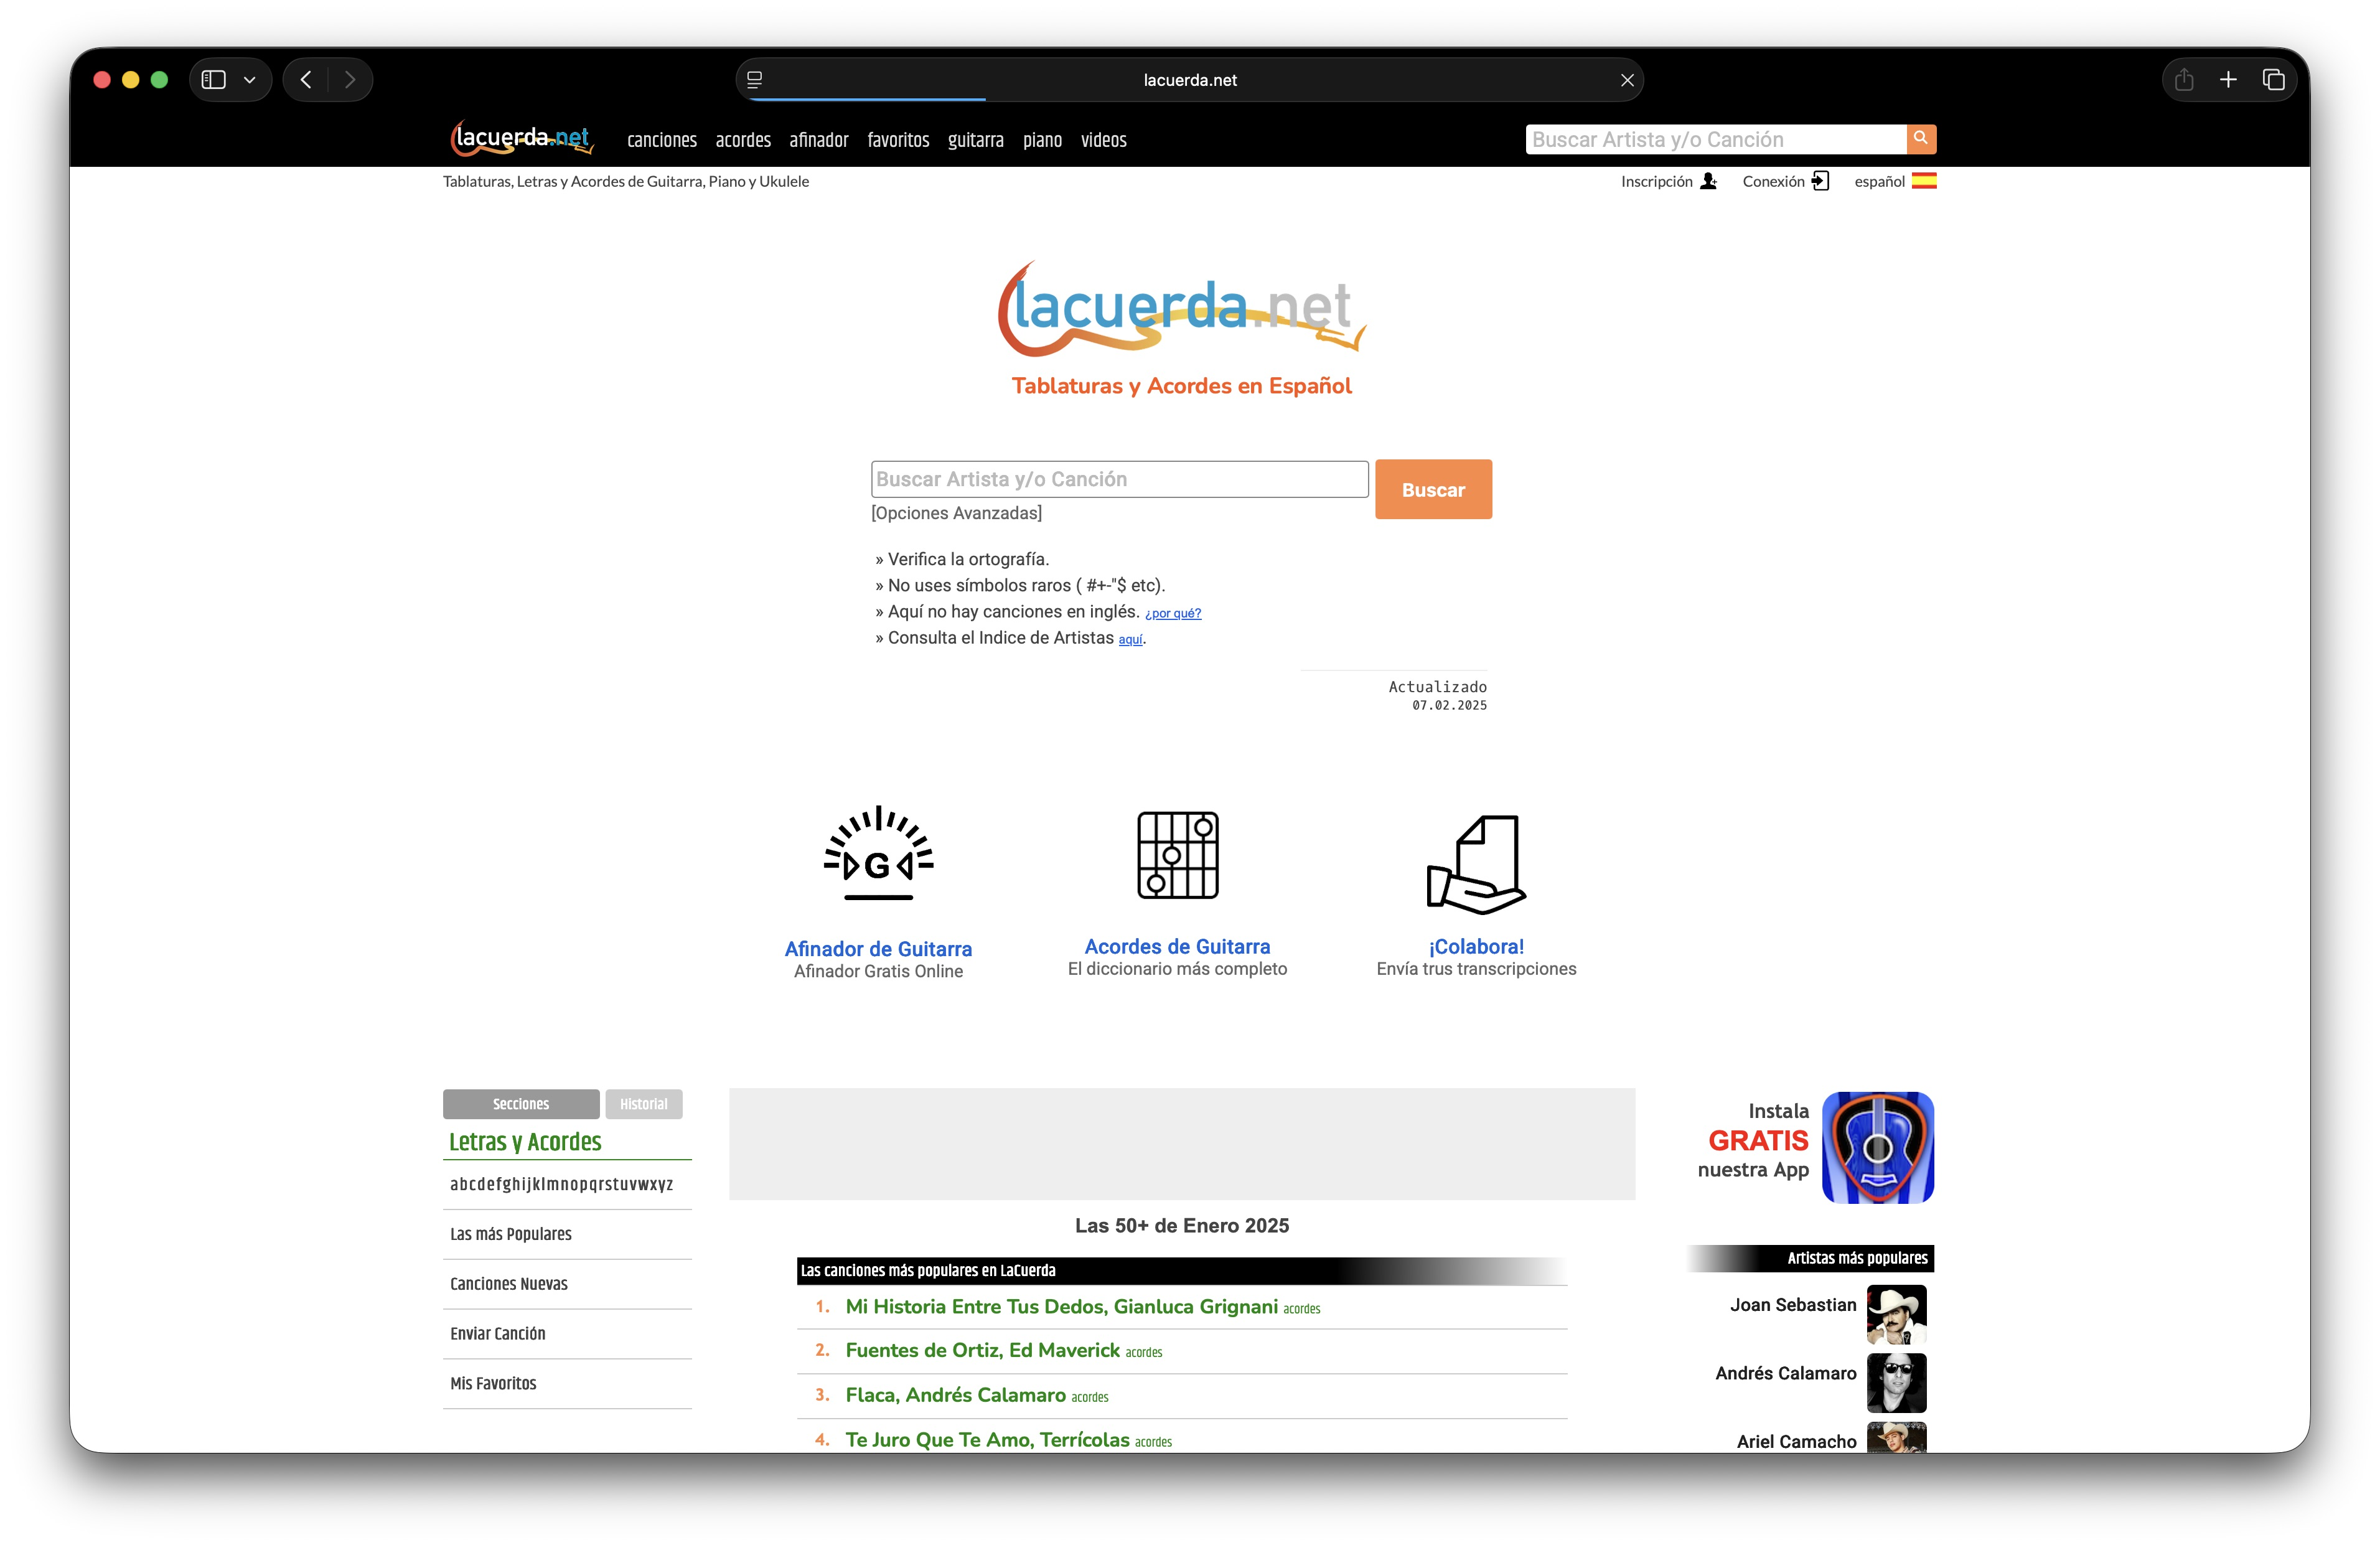
\includegraphics[width=\textwidth]{Ilustraciones/estado/lacuerdanet.jpeg}
        \caption{Página principal de LaCuerda~\cite{lacuerdanet_home}}\label{fig:lacuerdanet_home}
    \end{subfigure}
    \hfill
    \begin{subfigure}[t]{0.48\textwidth}
        \centering
        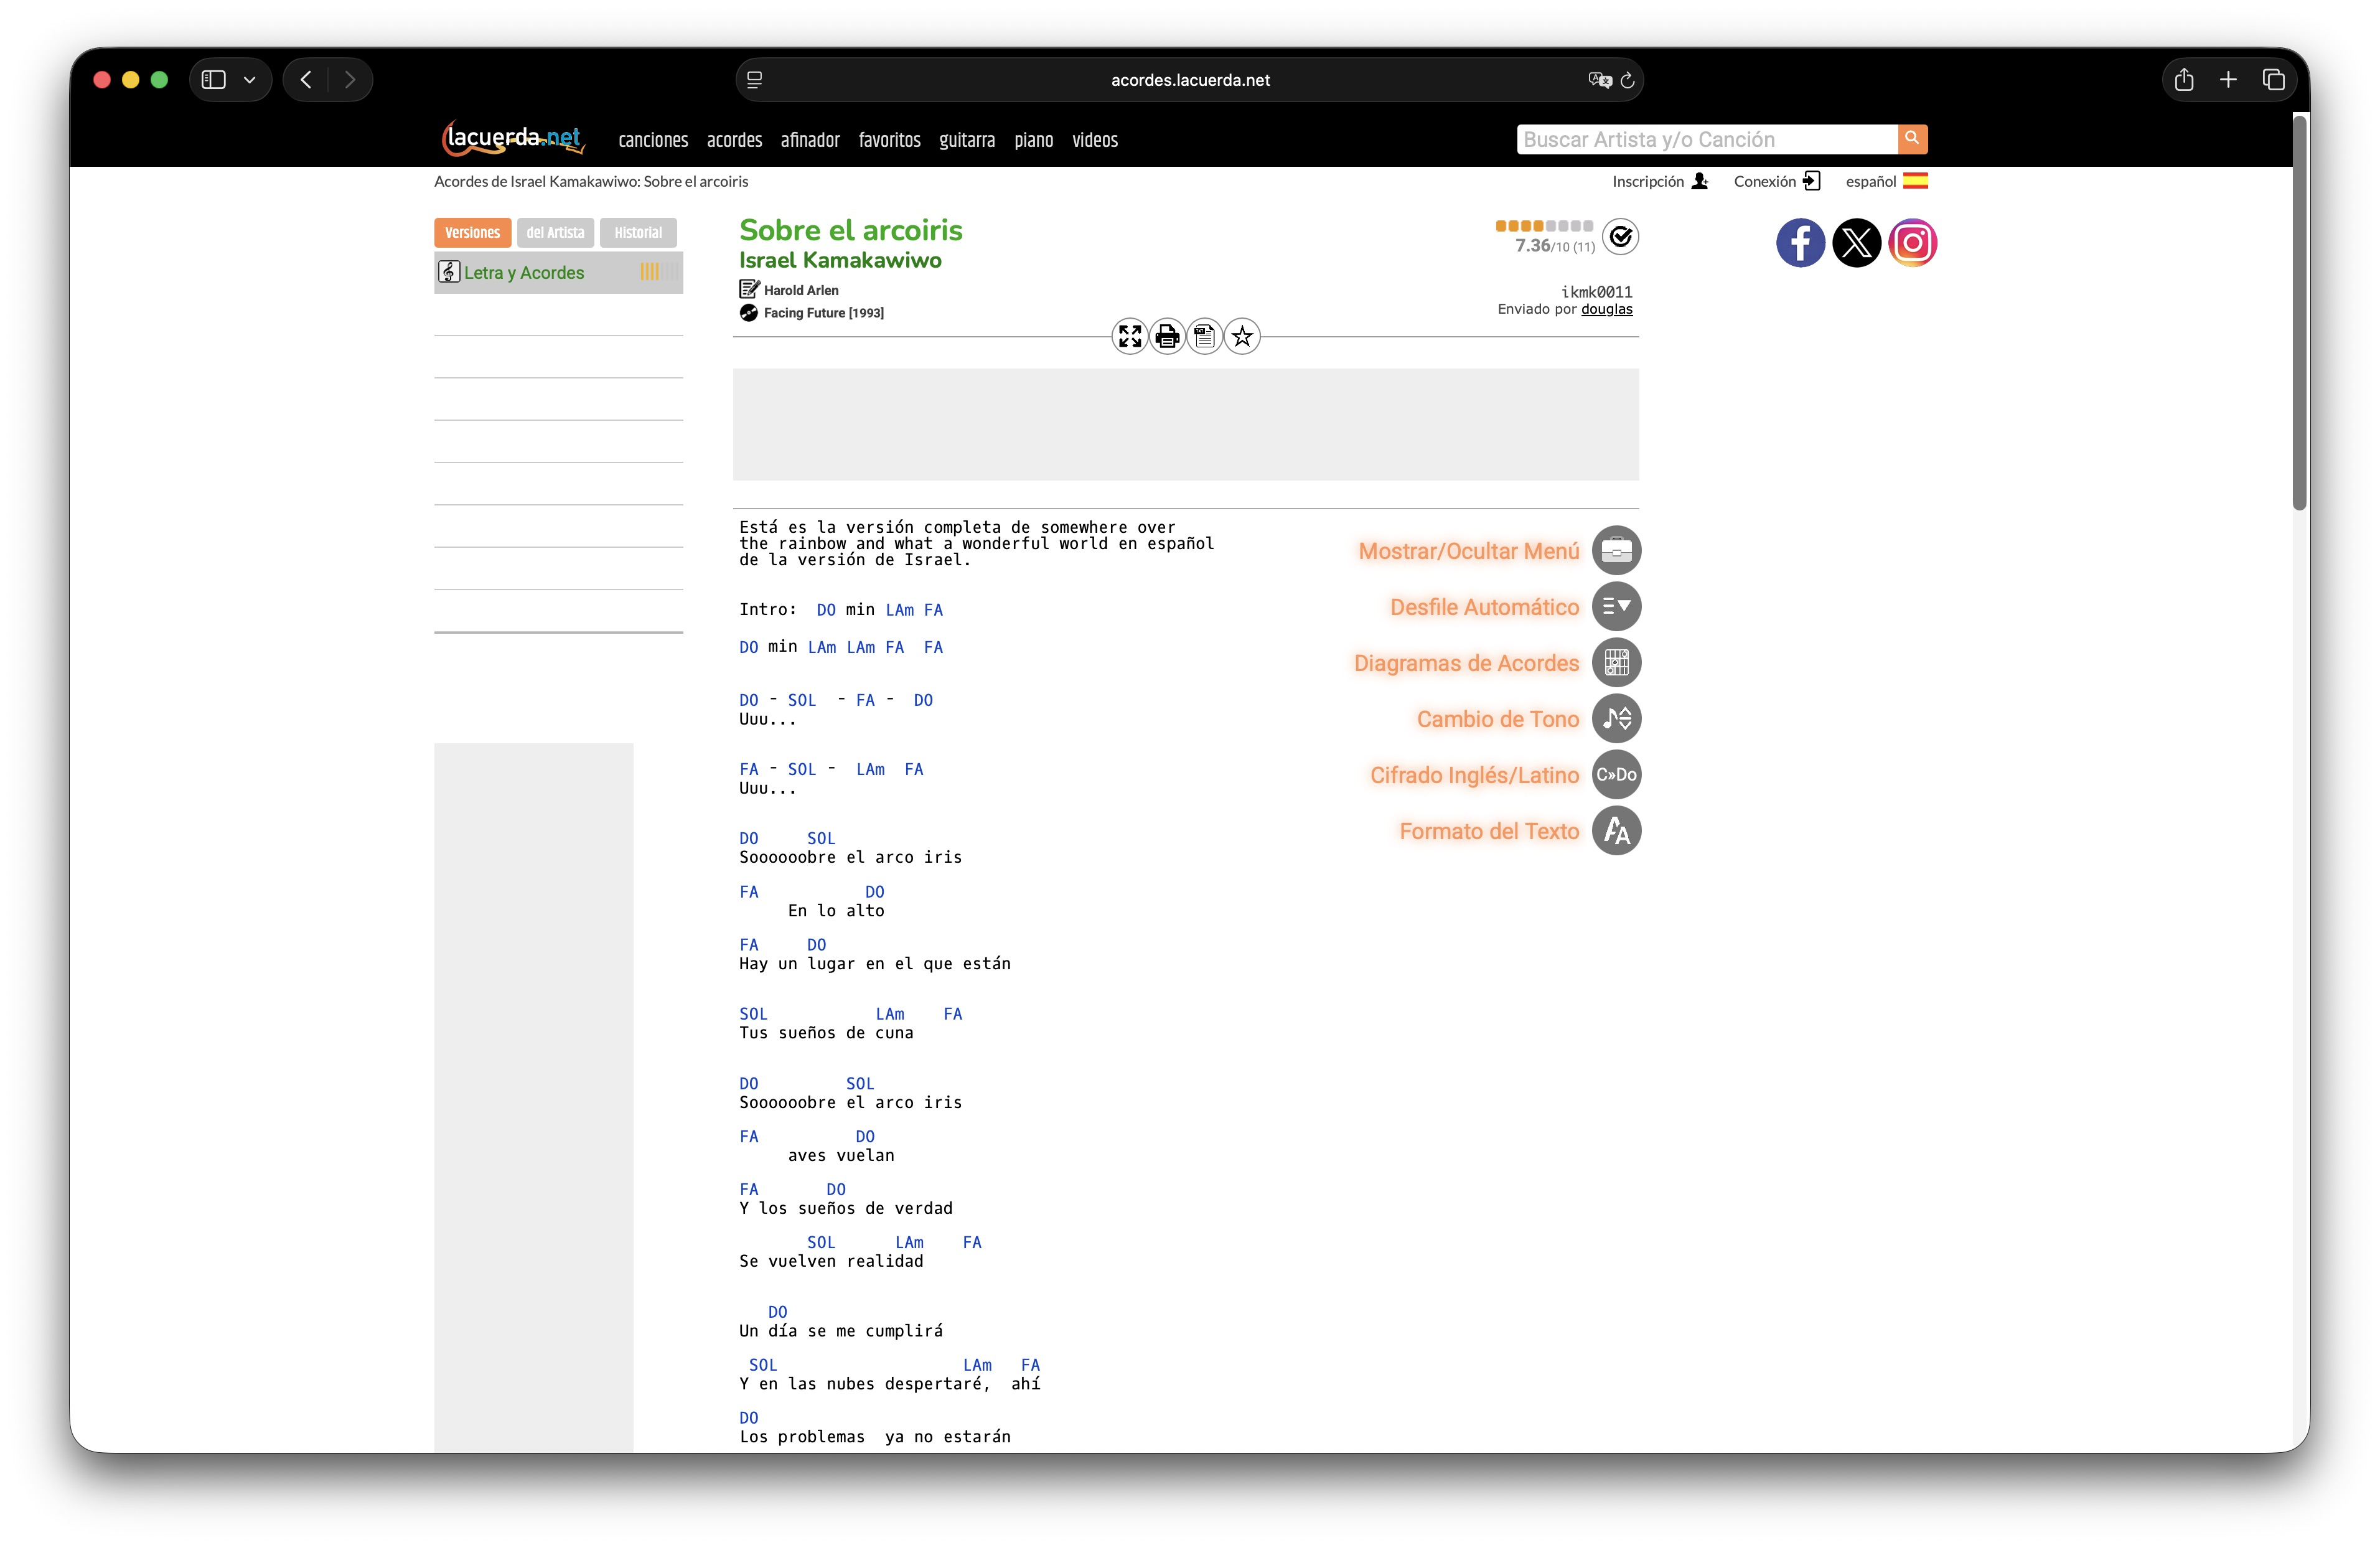
\includegraphics[width=\textwidth]{Ilustraciones/estado/lacuerdanet_somewhereovertherainbow.jpeg}
        \caption{Acordes y letra de \emph{Somewhere over the rainbow}~\cite{lacuerdanet_somewhereovertherainbow} para guitarra en LaCuerda}
        \label{fig:lacuerdanet_somewhereovertherainbow}
    \end{subfigure}
    \vspace{1em} % Espacio vertical entre filas

    % Segunda fila
    \begin{subfigure}[t]{0.48\textwidth}
        \centering
        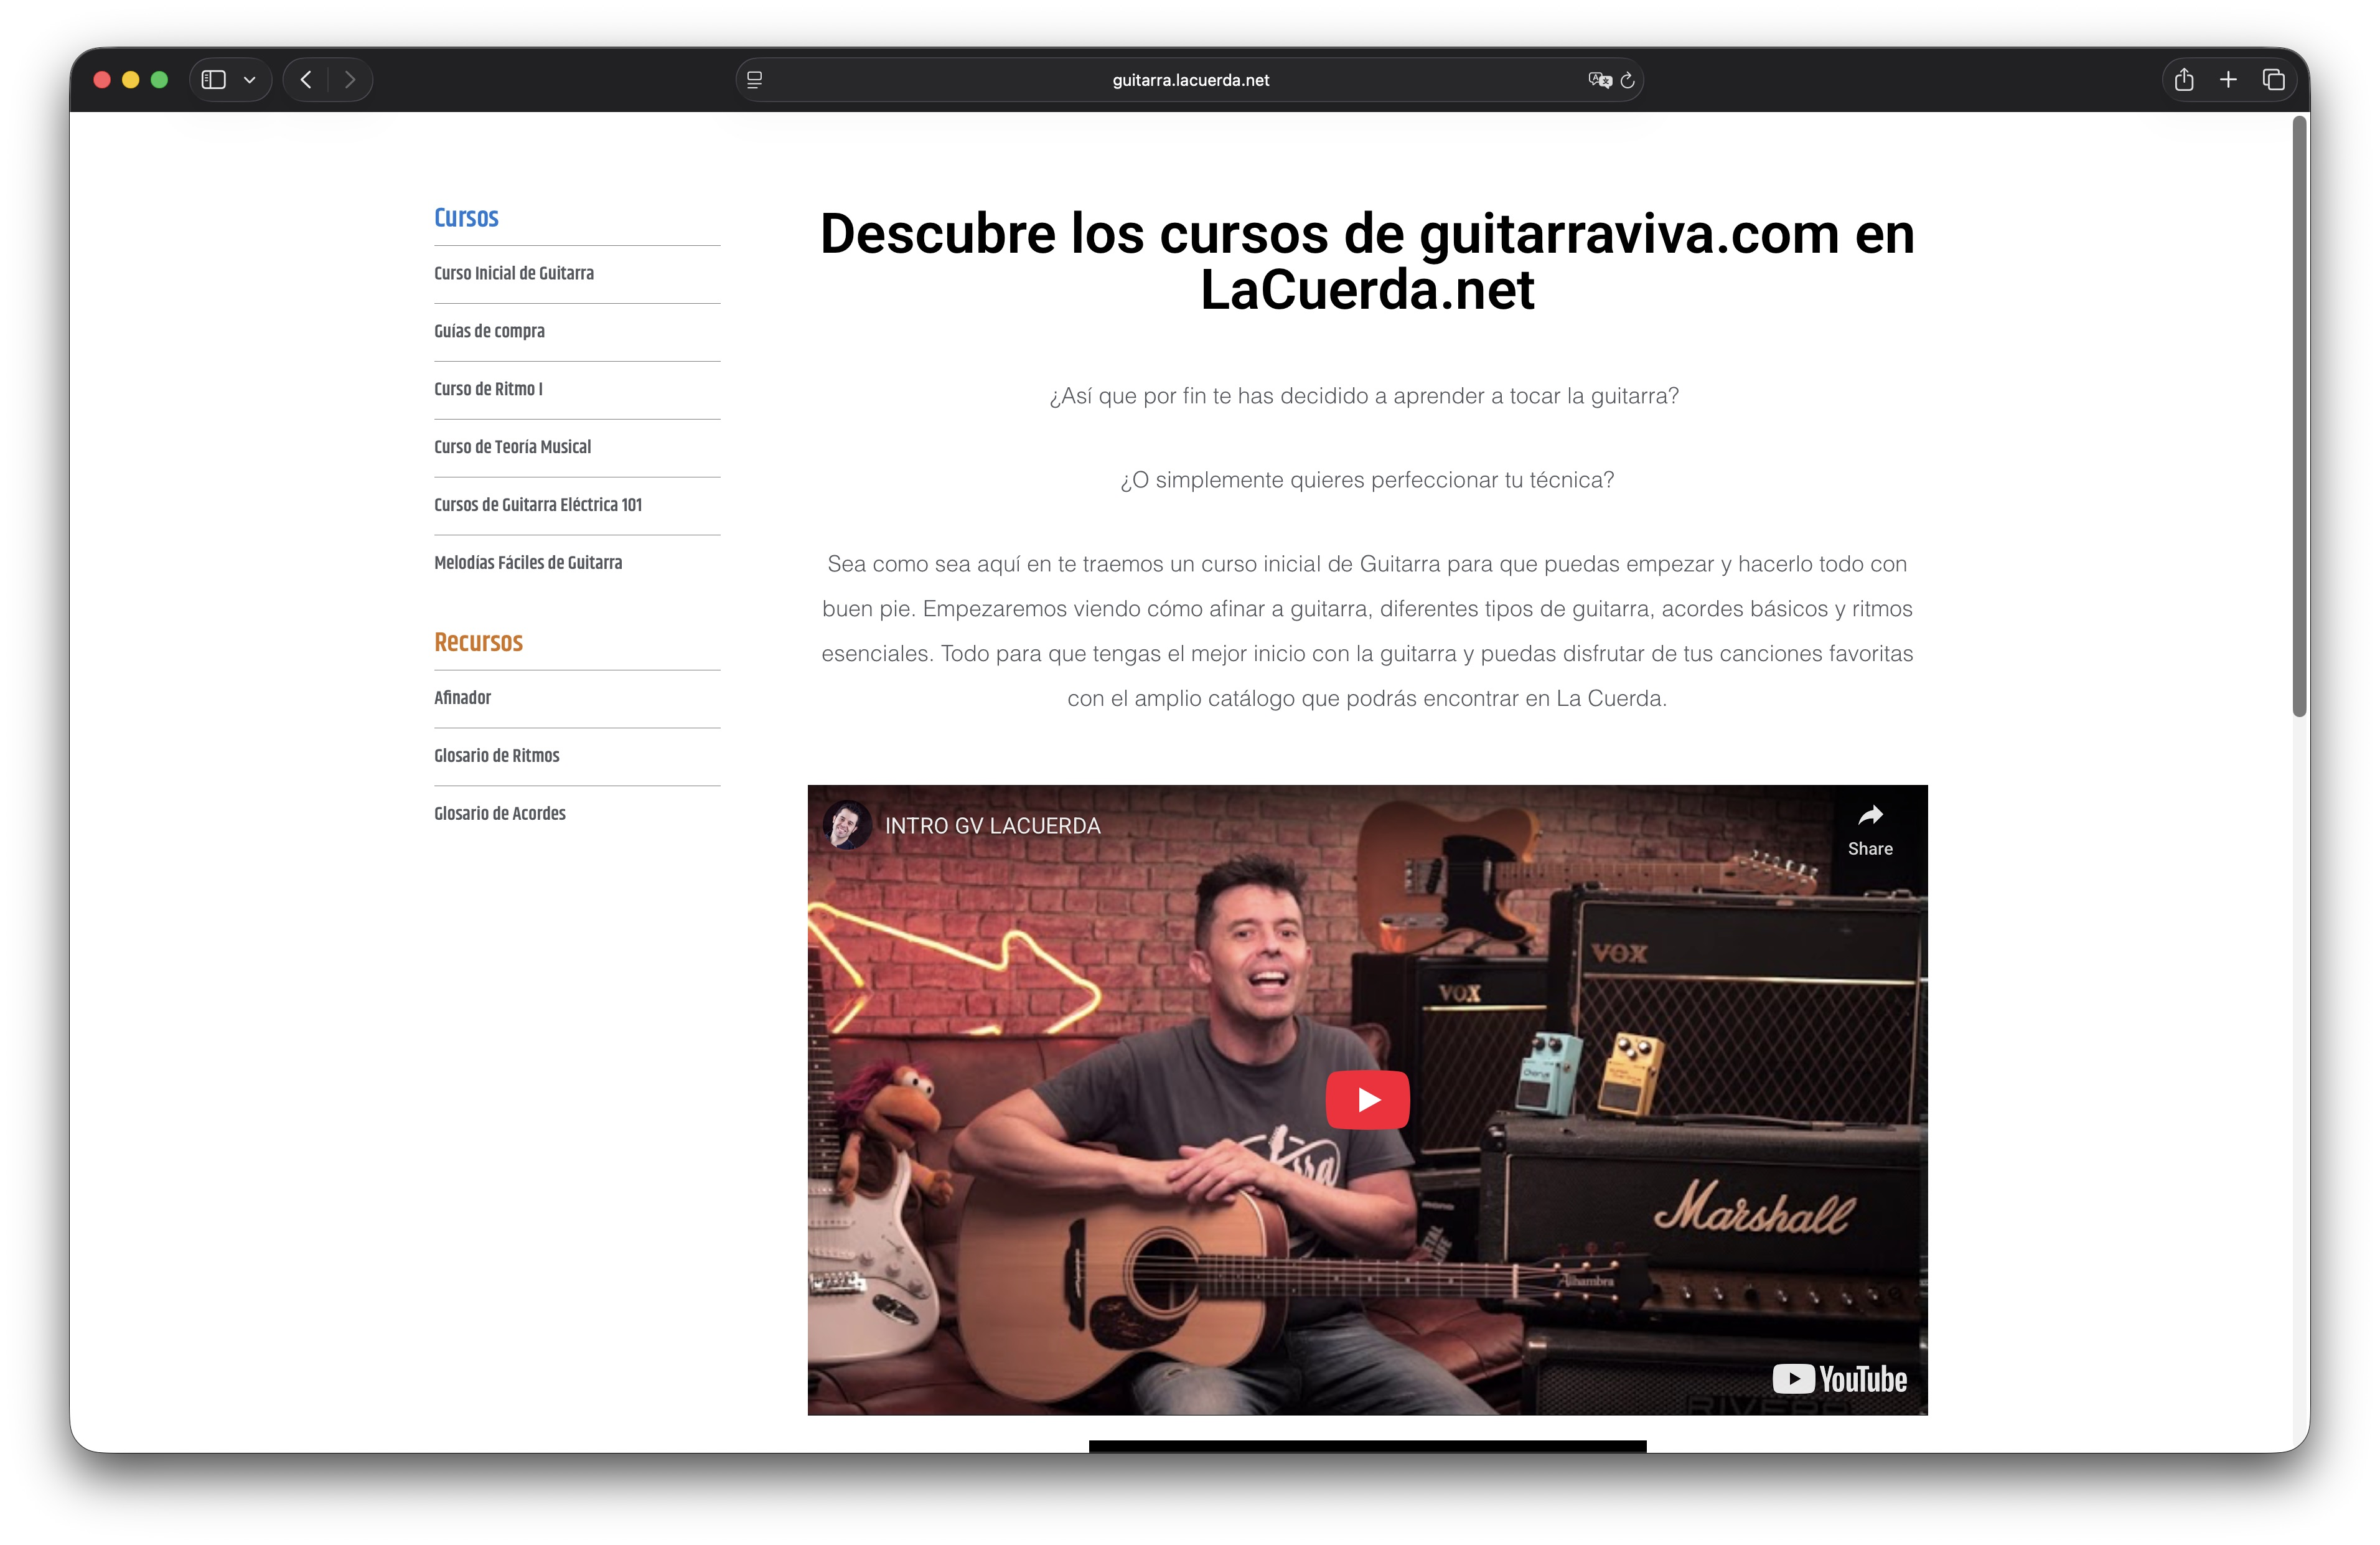
\includegraphics[width=\textwidth]{Ilustraciones/estado/lacuerdanet_cursos.jpeg}
        \caption{Página de cursos de LaCuerda~\cite{lacuerdanet_courses}}
        \label{fig:lacuerdanet_courses}
    \end{subfigure}
    \begin{subfigure}[t]{0.48\textwidth}
        \centering
        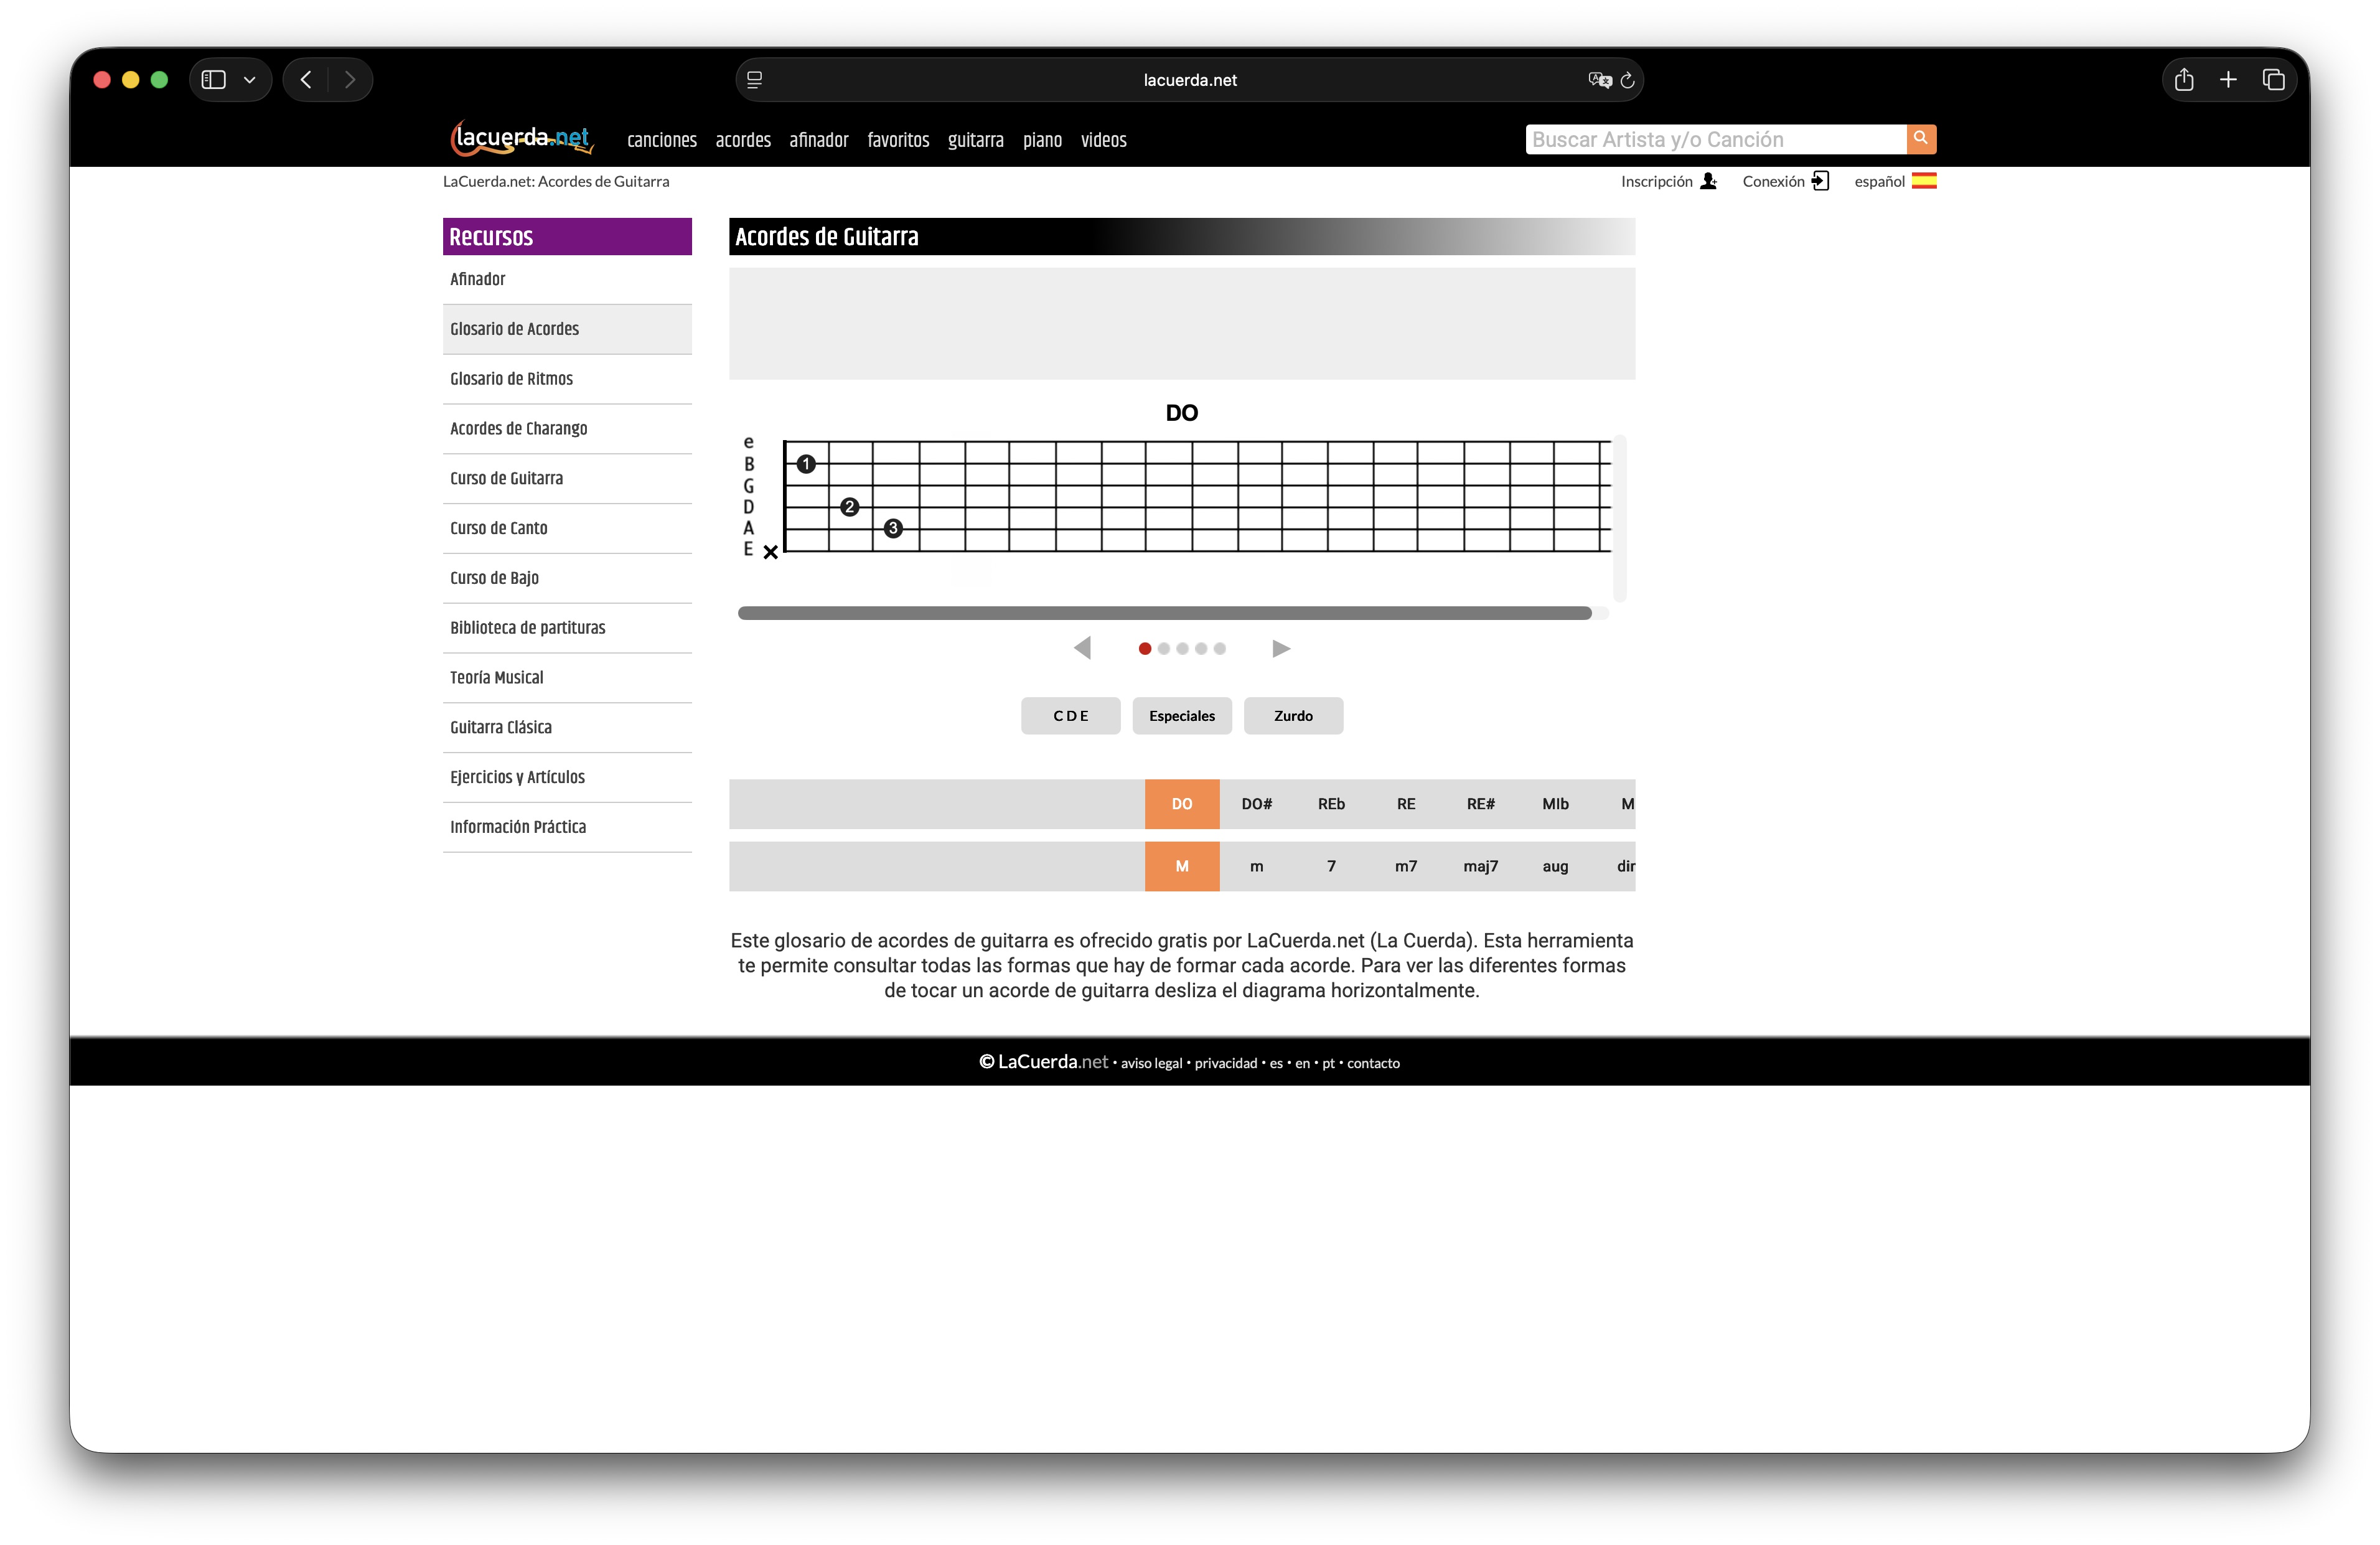
\includegraphics[width=\textwidth]{Ilustraciones/estado/lacuerdanet_acordes.jpeg}
        \caption{Página de cursos de LaCuerda~\cite{lacuerdanet_acordes}}
        \label{fig:lacuerdanet_acordes}
    \end{subfigure}

    \caption{Páginas de LaCuerda.}
    \label{fig:lacuerdanet_canciones}
\end{figure}

LaCuerda es en conclusión, una aplicación web que cuenta con una interfaz de apariencia anticuada en comparación con las otras alternativas analizadas, ofreciendo practicamente las mismas herramientas. No obstante, dada su antigüedad, dispone de un amplio catálogo de recursos, desde canciones hasta lecciones para aprender a tocar distintos instrumentos. A pesar de su método de verificación de contenido a través de administradores, podemos encontrar distintas versiones de una misma canción, incluso otorgándole autoría a los usuarios que realizan las aportaciones. Además, su modelo de negoció a través de anuncios permite el acceso gratuito a la mayoría de sus funcionalidades, incluso sin registro previo (véase Tabla~\ref{tab:lacuerda_funcionalidades_usuario}).

\begin{table}[H]
    \scriptsize
    \begin{minipage}[t]{0.4\textwidth}
    \centering
    \caption{Utilidades presentes en publicaciones de LaCuerda}\label{tab:lacuerda_utilidades_canciones}
    \begin{tabular}{l c}
        \hline
        \textbf{Utilidad} & \textbf{Existe} \\
        \hline
        Transportador & \ding{51} \\
        Lista de acordes & \ding{51} \\
        Autodesplazamiento & \ding{51} \\
        Impresión/Descarga & \ding{51} \\
        Cambio de notación & \ding{51}  \\
        Cambio de instrumento & \ding{51}  \\
        Guardar canción & \ding{51} \\
        Guía de rasgueos & \\
        \hline
    \end{tabular}
    \end{minipage}
\hfill
\begin{minipage}[t]{0.56\textwidth}
    \centering
    \caption{Funcionalidades disponibles según el rol del usuario de LaCuerda}\label{tab:lacuerda_funcionalidades_usuario}
    \begin{tabular}{l c c }
        \hline
        \multirow{2}{*}{\textbf{Funcionalidad}} & \multicolumn{2}{c}{\textbf{Rol Usuario}} \\
         & Visitante & Registrado \\
        \hline
        % --- Ejemplo de fila vacía (borra o completa) ---
        Biblioteca de canciones & \ding{51} & \ding{51} \\
        Creación y edición de publicaciones &  & \ding{51}  \\
        Utilidades de publicaciones & \ding{51} & \ding{51} \\
        Puntuar publicaciones &  & \ding{51}  \\
        Comentar publicaciones &  & \ding{51}  \\
        Solicitar nuevas canciones &  & \ding{51}  \\
        Cursos y guías & \ding{51} & \ding{51} \\
        Afinador & \ding{51} & \ding{51}  \\
        Calculadora de escalas y notas & &  \\
        Diccionario de acordes & \ding{51} & \ding{51}  \\
        % ------------------------------------------------
        \hline
    \end{tabular}
\end{minipage}
\end{table} 

\section{Comparación de aplicaciones web}

Según la información obtenida en el análisis anterior, podemos identificar una serie de funcionalidades comunes. No obstante, aunque las más populares son de nuestro interes \emph{(i.e. ya que nos indican lo que el usuario final puede esperar)}, a continuación nos centraremos en analizar las diferencias entre las aplicaciones:

Por un lado, en lo que respecta a las \textbf{utilidades presentes en las publicaciones de canciones} (véase Tabla~\ref{tab:comparativa_utilidades_canciones}), encontramos que la gran mayoría son ofrecidas por todas las aplicaciones. Si nos centramos en las utilidades que no son comunes en todas las páginas, podemos destacar las siguientes:

\begin{itemize}
    \item \textbf{Cambio de notación musical}, no disponible dada la popularidad de la notación inglesa en instrumentos de cuerda y al origen anglosajón de la mayoría de las aplicaciones. Solo LaCuerda ofrece la posibilidad de cambiar a notación latina, posiblemente por su origen hispanohablante.
    \item \textbf{Cambio de instrumento}, estando disponible en la mayoría de aplicaciones, salvo Ukulele Tabs que se centra exclusivamente en el ukelele.
    \item \textbf{Guía de rasgueos}, presente unicamente en Ukulele Tabs y Ultimate Guitar. Aunque no entraña dificultad técnica implementarla, la gran variedad de rasgueos posibles dificultar su inclusión en todas las aplicaciones.
\end{itemize}

\begin{table}[H]
    \centering
    \caption{Comparativa de utilidades en publicaciones por aplicación web.}\label{tab:comparativa_utilidades_canciones}
    \scriptsize
    \begin{tabular}{p{0.3\textwidth} c c c c}
        \hline
        \textbf{Utilidad} & \textbf{Ukulele Tabs} & \textbf{UkuTabs} & \textbf{Ultimate Guitar} & \textbf{LaCuerda} \\
        \hline
        Transportador & \ding{51} & \ding{51} & \ding{51} & \ding{51} \\
        Lista de acordes & \ding{51} & \ding{51} & \ding{51} & \ding{51} \\
        Autodesplazamiento & \ding{51} & \ding{51} & \ding{51} & \ding{51} \\
        Sistema de “me gusta” & \ding{51} & \ding{51} & \ding{51} & \ding{51} \\
        Sección de comentarios & \ding{51} & \ding{51} & \ding{51} & \ding{51} \\
        Impresión/Descarga & \ding{51} & \ding{51} & \ding{51} & \ding{51} \\
        Cambio de notación &  &  &  & \ding{51} \\
        Cambio de instrumento &  & \ding{51} & \ding{51} & \ding{51} \\
        Guardar canción & \ding{51} & \ding{51} & \ding{51} & \ding{51} \\
        Guía de rasgueos & \ding{51} &  & \ding{51} & \\
        \hline
    \end{tabular}
\end{table}

Por otro lado, en cuanto a las \textbf{funcionalidades generales de las aplicaciones web} (véase Tabla~\ref{tab:comparativa_funcionalidades}), podemos observar que la mayoría de aplicaciones ofrecen un conjunto similar de funcionalidades, siendo las únicas no comunes:

\begin{itemize}
    \item \textbf{Solicitud de nuevas canciones}, disponible en Ukulele Tabs, UkuTabs y LaCuerda. Ultimate Guitar no ofrece esta funcionalidad directamente, sino que lo hace a través de una sección de su foro.
    \item \textbf{Calculadora de escalas y notas}, presente en Ukulele Tabs y UkuTabs, posiblemente su ausencia se deba a la poca demanda de esta funcionalidad entre los usuarios de guitarra.
    \item \textbf{Diccionario de acordes}, disponible en Ukulele Tabs, UkuTabs y LaCuerda. Ultimate Guitar no ofrece esta funcionalidad debido a que ya sus publicaciones integran lista de acordes.
\end{itemize}

\begin{table}[H]
    \centering
    \caption{Comparativa de funcionalidades por aplicación web.}\label{tab:comparativa_funcionalidades}
    \scriptsize
    \begin{tabular}{p{0.3\textwidth} c c c c}
        \hline
        \textbf{Funcionalidad} & \textbf{Ukulele Tabs} & \textbf{UkuTabs} & \textbf{Ultimate Guitar} & \textbf{LaCuerda} \\
        \hline
        Biblioteca de canciones & \ding{51} & \ding{51} & \ding{51} & \ding{51} \\
        Publicaciones con letra y acordes & \ding{51} & \ding{51} & \ding{51} & \ding{51} \\
        Utilidades en publicaciones & \ding{51} & \ding{51} & \ding{51} & \ding{51} \\
        Impresión de publicaciones & \ding{51} & \ding{51} & \ding{51} & \ding{51} \\
        Creación y edición de publicaciones & \ding{51} & \ding{51} & \ding{51} & \ding{51} \\
        Puntuar publicaciones & \ding{51} & \ding{51} & \ding{51} & \ding{51} \\
        Comentar publicaciones & \ding{51} & \ding{51} & \ding{51} & \ding{51} \\
        Solicitar nuevas canciones & \ding{51} & \ding{51} &  & \ding{51} \\
        Cursos y guías & \ding{51} & \ding{51} & \ding{51} & \ding{51} \\
        Afinador & \ding{51} & \ding{51} & \ding{51} & \ding{51} \\
        Calculadora de escalas y notas & \ding{51} & \ding{51} &  &  \\
        Diccionario de acordes & \ding{51} & \ding{51} &  & \ding{51} \\
        \hline
    \end{tabular}
\end{table}

Podemos concluir que las utilidades y funcionalidades comunes son esenciales para el desarrollo de una aplicación web que siga el modelo de las páginas analizadas. Sin embargo, aquellas no comunes podrían ser consideradas como características adicionales que aporten valor añadido al producto final, diferenciándolo de la competencia.
\section{Alcance del proyecto}

En las secciones anteriores se ha realizado un estudio de mercado, identificando las aplicaciones web mas populares para otros instrumentos, listando y comparando sus utilidades y funcionalidades características, haciendo especial hincapié en aquellas funcionalidades menos comunes.

De este modo, se han seleccionado aquellas utilidades y funcionalidades que cimentarán la aplicación web a desarrollar, estableciendo prioridades según su importancia \tabref{tab:timpletabs_utilidades_canciones} y \tabref{tab:timpletabs_funcionalidades}.

\begin{table}[H]
    \scriptsize
    \begin{minipage}[t]{0.48\textwidth}
        \centering
        \caption{Prioridad de utilidades para TimpleTabs}\label{tab:timpletabs_utilidades_canciones}
        \begin{tabular}{l c c c}
            \hline
            \multirow{2}{*}{\textbf{Utilidad}} & \multicolumn{3}{c}{\textbf{TimpleTabs}} \\
             & Baja & Media & Alta \\
            \hline
            Transportador &  & \ding{51} & \\
            Lista de acordes &   & & \ding{51} \\
            Autodesplazamiento  &  & & \ding{51} \\
            Impresión/Descarga  & \ding{51} & & \\
            Cambio de notación  & & & \ding{51} \\
            Cambio de instrumento & - & - & - \\
            Guardar canción  &\ding{51} & & \\
            Guía de rasgueos & & \ding{51} & \\
            \hline
        \end{tabular}
    \end{minipage}
    \hfill
    \begin{minipage}[t]{0.48\textwidth}
        \centering
        \caption{Prioridad de funcionalidades para TimpleTabs}\label{tab:timpletabs_funcionalidades}
        \begin{tabular}{p{0.48\textwidth} c c c }
            \hline
            \multirow{2}{*}{\textbf{Funcionalidad}} & \multicolumn{3}{c}{\textbf{TimpleTabs}} \\
            & Baja & Media & Alta \\
            \hline
            Biblioteca de canciones & &  & \ding{51} \\
            Creación y edición de publicaciones & & & \ding{51} \\
            Utilidades en publicaciones & & &  \ding{51} \\
            Comentar publicaciones & &  \ding{51} & \\
            Puntuar publicaciones & &  \ding{51} & \\
            Solicitar nuevas canciones & \ding{51} & & \\
            Cursos y guías &  & \ding{51} & \\
            Afinador &  & \ding{51} & \\
            Calculadora de escalas y notas & & & \ding{51} \\
            Diccionario de acordes & & & \ding{51} \\
            \hline
        \end{tabular}
    \end{minipage}
\end{table}

Utilizando como referencia lo anterior, se han especificado una serie de requisitos funcionales y no funcionales \tabref{tab:requisitosfuncionales} y \tabref{tab:requisitosnofuncionales}. Estos requisitos definen el alcance del proyecto, sirviendo además como apoyo durante el desarrollo de modo que todas las funcionalidades implementadas cumplan con los objetivos establecidos.

\begin{table}[H]
    \centering
    \scriptsize
    \begin{tabular}{l p{0.58\textwidth} p{0.24\textwidth} l}
        \textbf{ID} & \textbf{Requisito Funcional} & \textbf{Funcionalidad} & \textbf{Prio.} \\ \hline
        RF1  & El usuario debe poder iniciar y cerrar sesión. & Cuenta de usuario & Alta \\ \hline
        RF2  & El usuario debe poder registrarse utilizando su correo electrónico, contraseña y un nombre de usuario. & Cuenta de usuario & Alta \\ \hline
        RF3  & El usuario debe poder modificar su perfil. & Cuenta de usuario & Alta \\ \hline
        RF4  & El usuario debe poder recuperar o restablecer su contraseña en caso de olvido. & Cuenta de usuario & Alta \\ \hline
        RF5  & El sistema debe validar que toda publicación incluya al menos título, letra y acordes. & Crear y editar publicaciones & Alta \\ \hline
        RF6  & El usuario debe poder crear publicaciones en respuesta a solicitudes realizadas por otros usuarios. & Crear y editar publicaciones & Alta \\ \hline
        RF7  & El usuario debe poder crear, editar y eliminar sus propias publicaciones. & Crear y editar publicaciones & Alta \\ \hline
        RF8  & El usuario debe poder visualizar una lista de acordes en las publicaciones. & Utilidades en publicaciones & Alta \\ \hline
        RF9  & El usuario debe poder activar y desactivar el autoscroll en una publicación. & Utilidades en publicaciones & Alta \\ \hline
        RF10 & El usuario debe poder seleccionar una notación musical preferida. & Utilidades en publicaciones & Alta \\ \hline
        RF12 & El usuario debe poder transportar los acordes de una publicación. & Utilidades en publicaciones & Media \\ \hline
        RF13 & El usuario debe poder ver guías de rasgueos. & Utilidades en publicaciones & Media \\ \hline
        RF14 & El usuario debe poder compartir publicaciones mediante enlace o redes sociales. & Utilidades en publicaciones & Media \\ \hline
        RF15 & El usuario debe poder imprimir o descargar una publicación. & Utilidades en publicaciones & Baja \\ \hline
        RF16 & El usuario debe poder visualizar una biblioteca de canciones. & Biblioteca de canciones & Alta \\ \hline
        RF17 & El usuario debe poder acceder a una calculadora de escalas y notas. & Calculadora de escalas y notas & Alta \\ \hline
        RF18 & El usuario debe poder acceder a un diccionario de acordes. & Diccionario de acordes & Alta \\ \hline
        RF19 & El usuario debe poder acceder a un afinador interactivo. & Afinador & Media \\ \hline
        RF20 & El afinador interactivo debe mostrar cuerdas, afinación objetivo y afinación actual. & Afinador & Alta \\ \hline
        RF21 & El usuario debe poder comentar en publicaciones. & Comentar publicaciones & Media \\ \hline
        RF22 & El usuario debe poder puntuar una publicación. & Puntuar publicaciones & Media \\ \hline
        RF23 & El usuario debe poder acceder a páginas informativas sobre el instrumento. & Cursos y guías & Media \\ \hline
        RF24 & El usuario debe poder guardar canciones en su carpeta personal. & Guardar canciones & Baja \\ \hline
        RF25 & El usuario debe poder solicitar canciones. & Solicitar nuevas canciones & Baja \\ \hline
    \end{tabular}
    \caption{Requisitos Funcionales de la aplicación web corregidos}\label{tab:requisitosfuncionales}
\end{table}


\begin{table}[H]
\centering
\scriptsize
\begin{tabular}{l p{0.84\textwidth} l}
\textbf{ID} & \textbf{Requisito No Funcional} & \textbf{Prio.} \\ \hline
RNF1 & El sistema debe ser responsivo, adaptándose a diferentes tamaños de pantalla y dispositivos. & Alta \\ \hline
RNF2 & El sistema debe incluir una descripción textual (alt) en todas las imágenes. & Alta \\ \hline
RNF3 & El sistema debe incluir un aria-label o aria-labelledby en todos los elementos interactivos, describiendo su función para lectores de pantalla. & Alta \\ \hline
RNF4 & El sistema debe proporcionar navegación mediante un encabezado (header) y un pie de página (footer) consistentes en todas las vistas. & Alta \\
\end{tabular}
\caption{Requisitos No Funcionales de la aplicación web}\label{tab:requisitosnofuncionales}
\end{table}

%% En capítulos anteriores se ha hablado sobre los objetivos, la metodología, la planificación y analizado el estado y alternativas actuales en las que se desarrolla el proyecto. Utilizando como referencia las funcionalidades y utilidades identificadas anteriormente, podemos esbozar el alcance mínimo del proyecto \tabref{tab:timpletabs_utilidades_canciones} y \tabref{tab:timpletabs_funcionalidades}.

%% Las funcionalidades y utilidades conformarán los cimientos de la aplicación web, que gracias a la metodlogía seleccionada, podrá transformarse en el proceso.

%% En conclusión, la aplicación web tiene como alcance la implementación de las funcionalidades mínimas para el objetivo de creación, difusión y práctica de canciones para timple, siendo este último el protagonista que se tendrá en cuenta en decisiones como el diseño, la experiencia y el desarrollo.

\chapter{Normativa y legislación}
Este capítulo se centra en los aspectos legales que rodean al proyecto, así como la normativa y legislación vigente.


\chapter{Tecnologías y herramientas utilizadas}

Este capítulo expone las tecnologías y herramientas utilizadas durante el desarrollo del proyecto, así como las licencias de uso.

\section{Programas}
\begin{table}[H]
    \centering
    \caption{Herramientas utilizadas y sus licencias}
    \small
    \begin{tabular}{l l l}
    \hline
    \textbf{Categoría} & \textbf{Herramienta} & \textbf{Licencia} \\
    \hline
    \multirow{3}{*}{Diseño gráfico} & Affinity Designer & Licencia comercial (pago único) \\
                                   & Affinity Photo    & Licencia comercial (pago único) \\
                                   & Figma             & Plan gratuito \\
    \hline
    \multirow{2}{*}{Desarrollo web} & Visual Studio Code & MIT~\cite{vscode_license} \\
    & Next.js           & MIT~\cite{nextjs_license} \\
    \hline
    Bases de datos & Supabase & Apache 2.0~\cite{supabase_license} \\
    \hline
    \multirow{2}{*}{Control de versiones} & Git      & GPLv2~\cite{git_license} \\
     & GitHub   & Propietaria / Free tier~\cite{github_license} \\
    \hline
    Redacción & LaTeX             & LaTeX Project Public License~\cite{latex_license} \\
    \hline
    \end{tabular}
    \label{tab:herramientas_licencias}
\end{table}


\section{Otras tecnologías}

\chapter{Desarrollo}
Este capítulo cubre el desarrollo, exponiendo las distintas fases y tareas ejecutadas para la implementación de la aplicación web.

\section{Incremento 1}
Este primer incremento se centra en la configuración del proyecto y implementación de registro, autenticación y perfil de usuario.

\subsection{Análisis}
Con respecto a la \textbf{configuración del proyecto}, se ha decidido utilizar la plataforma backend \emph{Supabase} y los frameworks \emph{Next.js} para el desarrollo de la aplicacion web y \textit{Tailwind CSS} para el manejo de estilos. Como punto de partida, se ha utilizado la plantilla \emph{Next.js Supabase Auth Starter} \cite{nextjs_supabase_starter}, la cual incluye la configuración básica para el registro y autenticación de usuarios mediante \emph{Supabase}.

Por otro lado, en cuanto a la \textbf{implementación de registro, autenticación y perfil de usuario}, se han desarrollado los requisitos funcionales y no funcionales definidos en \tabref{tab:requisitosfuncionalesincremento1} y no funcionales \tabref{tab:requisitosnofuncionales}.

\begin{table}[H]
    \centering
    \scriptsize
    \begin{tabular}{l p{0.58\textwidth} p{0.20\textwidth} l}
        \textbf{ID} & \textbf{Requisito Funcional} & \textbf{Funcionalidad} & \textbf{Prioridad} \\ \hline
        RF1  & El usuario debe poder iniciar y cerrar sesión. & Cuenta de usuario & Alta \\ \hline
        RF2  & El usuario debe poder registrarse utilizando su correo electrónico, contraseña y un nombre de usuario. & Cuenta de usuario & Alta \\ \hline
        RF3  & El usuario debe poder modificar su perfil. & Cuenta de usuario & Alta \\ \hline
        RF4  & El usuario debe poder recuperar o restablecer su contraseña en caso de olvido. & Cuenta de usuario & Alta \\ \hline
    \end{tabular}
    \caption{Requisitos Funcionales desarrollados en el incremento 1}\label{tab:requisitosfuncionalesincremento1}
\end{table}

\begin{table}[H]
    \centering
    \scriptsize
    \begin{tabular}{l p{0.79\textwidth} l}
    \textbf{ID} & \textbf{Requisito No Funcional} & \textbf{Prioridad} \\ \hline
    RNF1 & El sistema debe ser responsivo, adaptándose a diferentes tamaños de pantalla y dispositivos. & Alta \\ \hline
    RNF2 & El sistema debe incluir una descripción textual (alt) en todas las imágenes. & Alta \\ \hline
    RNF3 & El sistema debe incluir un aria-label o aria-labelledby en todos los elementos interactivos, describiendo su función para lectores de pantalla. & Alta \\ \hline
    RNF4 & El sistema debe proporcionar navegación mediante un encabezado (header) y un pie de página (footer) consistentes en todas las vistas. & Alta \\
    \end{tabular}
    \caption{Requisitos No Funcionales desarrollados en el incremento 2}\label{tab:requisitosnofuncionales}
\end{table}

\subsection{Diseño de datos}
La estructura de datos inicial se basa en la tabla de usuarios predeterminada de \emph{Supabase}, la cual incluye los campos mínimos necesarios para la autenticación de usuarios (destacamos id, email, contraseñas y fecha de creación). Por otro lado, se ha añadido una tabla adicional denominada \emph{profiles} para almacenar información adicional de los usuarios (para este primer incremento solo se ha incluido el nombre de usuario y fecha de creación). Las tablas de \emph{usuarios} y \emph{profiles} están directamente relacionadas entre sí, tal y como podemos observar en \figref{fig:diagrama_datos_i1}.

\begin{figure}[H]
    \centering
    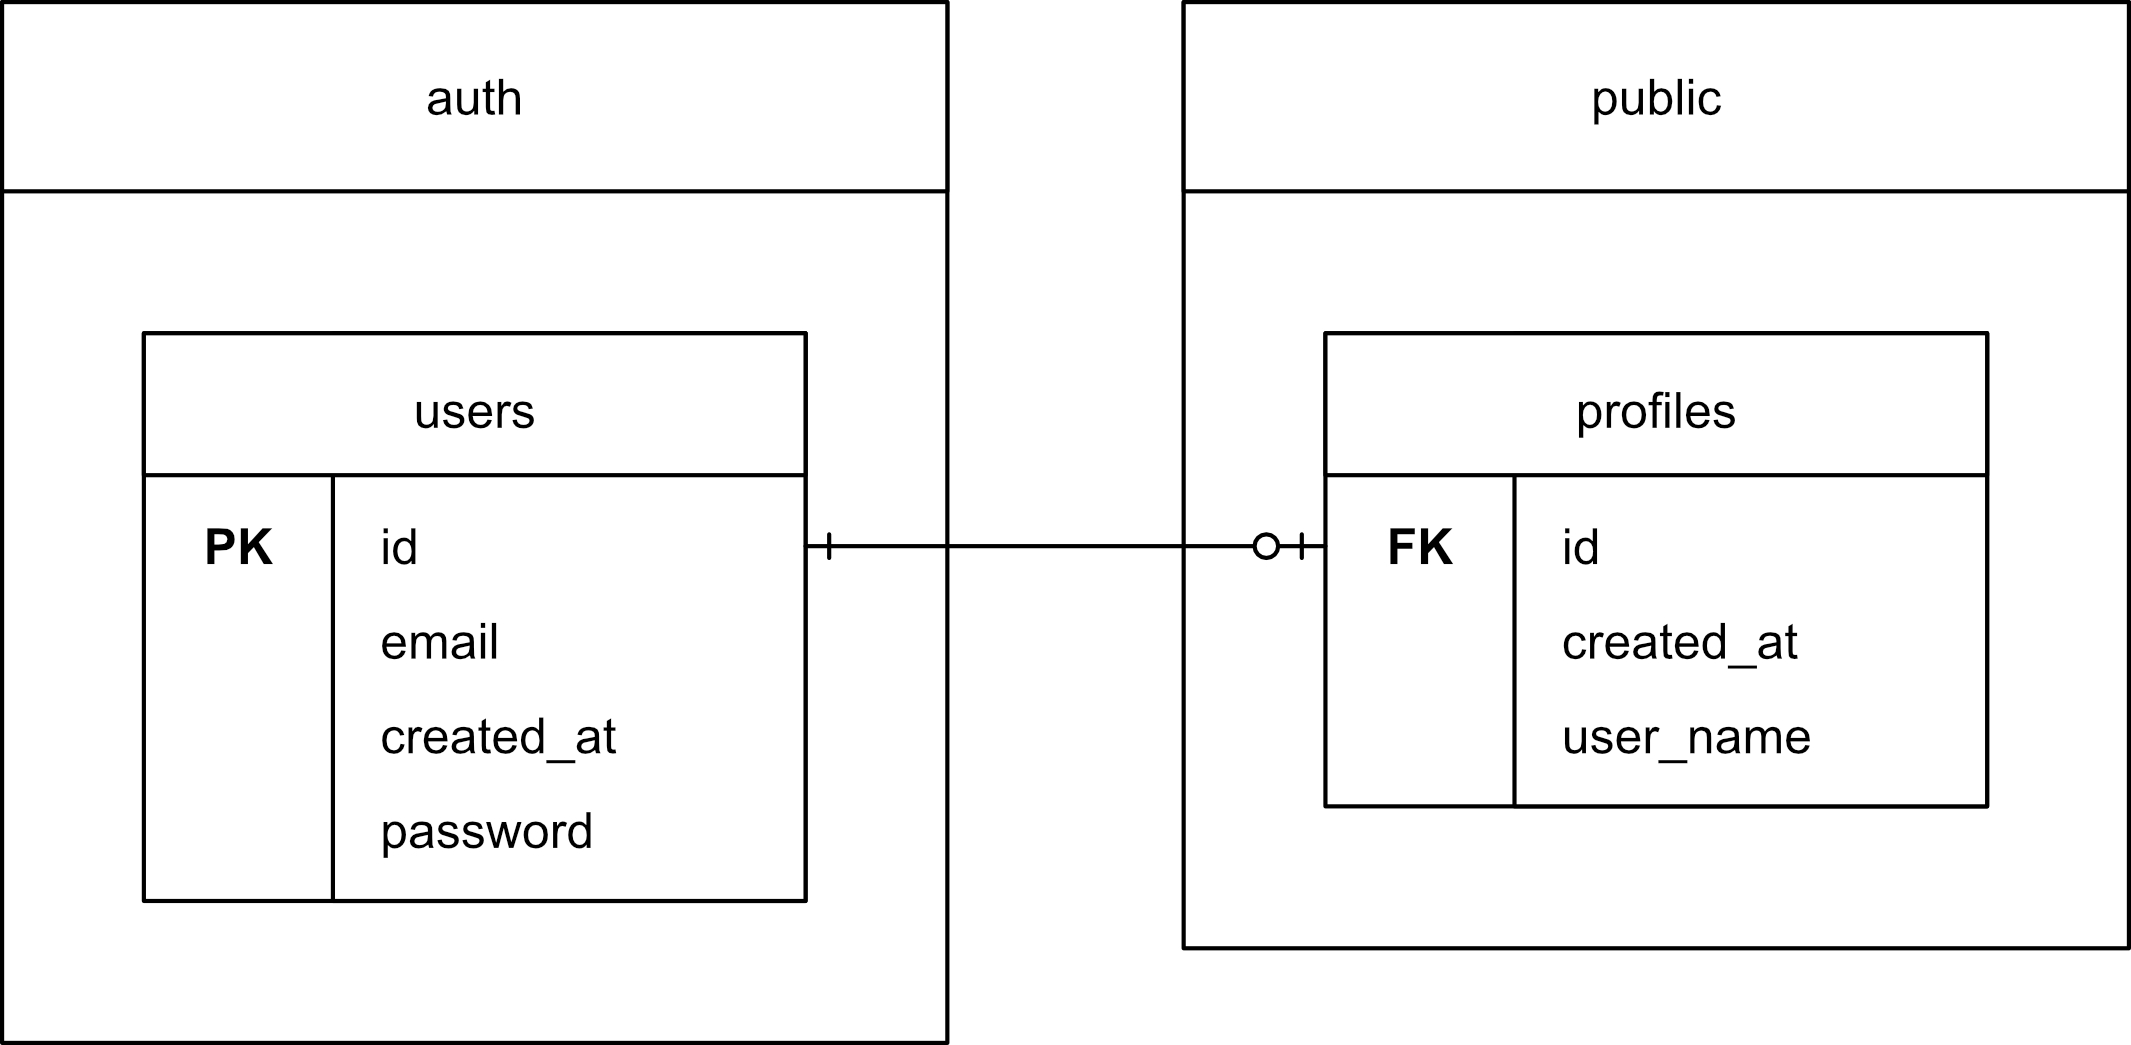
\includegraphics[width=0.8\textwidth]{Ilustraciones/desarrollo/incremento1/diagrama_datos_i1.jpg}
    \caption{Diagrama de estructura de datos de los perfiles de usuario}\label{fig:diagrama_datos_i1}
\end{figure}

\subsection{Diseño de interfaz}
Al tratarse del primer incremento, fué de vital importancia comenzar a definir la guía de diseño de la interfaz. En primer lugar, se estableció una paleta de colores con tonalidades de grises y azules \figref{fig:ui_palette}. Seguidamente se definió la guía de colores \figref{fig:ui_guide}, estableciendo los colores según su función (fondos, textos, primarios, etc.), con sus respectivos colores principales y de primer plano.

\begin{figure}[H]
    \centering
    \begin{subfigure}[t]{0.48\textwidth}
        \centering
        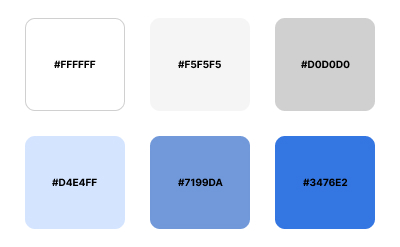
\includegraphics[width=1\textwidth]{Ilustraciones/desarrollo/incremento1/diseño/color_palette.jpg}
        \caption{Paleta de colores}\label{fig:ui_palette}
    \end{subfigure}
    \hfill
    \begin{subfigure}[t]{0.48\textwidth}
        \centering
        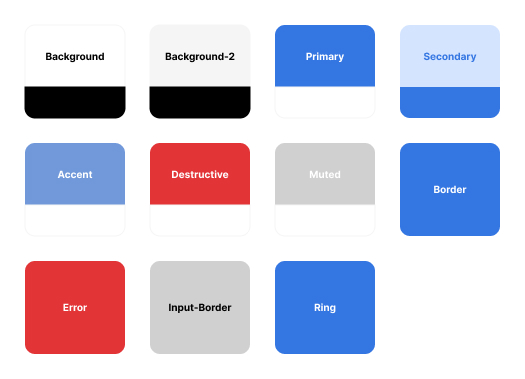
\includegraphics[width=\textwidth]{Ilustraciones/desarrollo/incremento1/diseño/color_scheme.jpg}
        \caption{Guía de colores. Arriba principal, abajo primer plano.}\label{fig:ui_guide}
    \end{subfigure}\caption{Colores utilizados en la interfaz}\label{fig:ui_colors}
\end{figure}

En segundo lugar, se diseñó el isologo de la aplicación web \figref{fig:ui_logo}, el cual combina el timple con el nombre de la aplicación web \emph{Timple Tabs}.

\begin{figure}[H]
    \centering
    
\includegraphics[width=0.5\textwidth]{Ilustraciones/desarrollo/incremento1/diseño/logo_2.png}
    \caption{Isologo de la aplicación web}\label{fig:ui_logo}
\end{figure}

En tercer lugar, se diseñaron algunos de los elementos comunes de la interfaz de usuario. Para este primer incremento fué fundamental el diseño de botones \figref{fig:ui_buttons} y campos de formulario \figref{fig:ui_fields}, en los que se hace uso de los iconos de la biblioteca pública \emph{Lucide Icons} \cite{lucide_icons}.

\begin{figure}[H]
    \centering
    \begin{subfigure}[t]{0.48\textwidth}
        \centering
        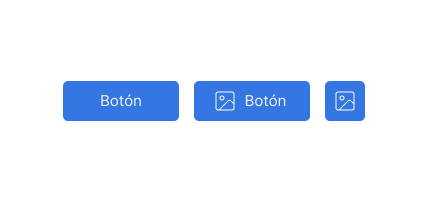
\includegraphics[width=1\textwidth]{Ilustraciones/desarrollo/incremento1/diseño/buttons.jpg}
        \caption{Botones y sus variantes según espacio}\label{fig:ui_buttons_variants}
    \end{subfigure}
    \hfill
    \begin{subfigure}[t]{0.48\textwidth}
        \centering
        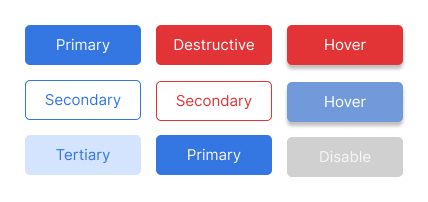
\includegraphics[width=1\textwidth]{Ilustraciones/desarrollo/incremento1/diseño/button_color_scheme.jpg}
        \caption{Botones y sus variantes según función y estado}\label{fig:ui_buttons_color}
    \end{subfigure}
    \vspace{1em}
    \begin{subfigure}[t]{\textwidth}{
        \centering
        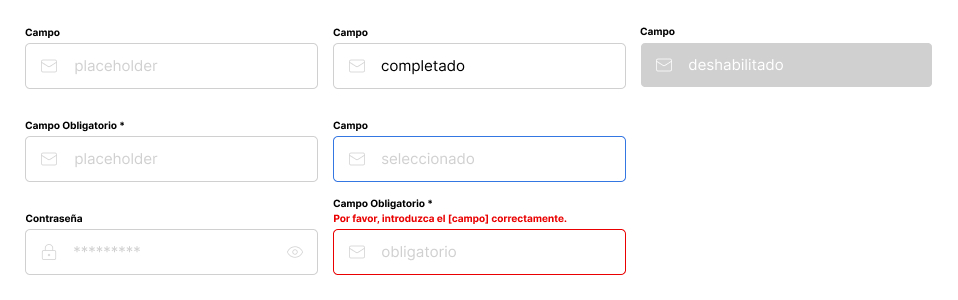
\includegraphics[width=\textwidth]{Ilustraciones/desarrollo/incremento1/diseño/fields.jpg}
        \caption{Campos y sus variantes según función y estado}\label{fig:ui_fields}}    
    \end{subfigure}
    \caption{Diseño de elementos comunes}\label{fig:ui_buttons}
\end{figure}

Finalmente, con todos los elementos mencionados anteriormente, se definió una básica guía de diseño que sirvió como referencia para el diseño de las pantallas correspondientes al registro, inicio de sesión \figref{fig:ui_login}, recuperación de contraseña \figref{fig:passrec} y registro \figref{fig:ui_register}. 

\begin{figure}[H]
    \centering
    \begin{subfigure}[t]{0.3\textwidth}
        \centering
        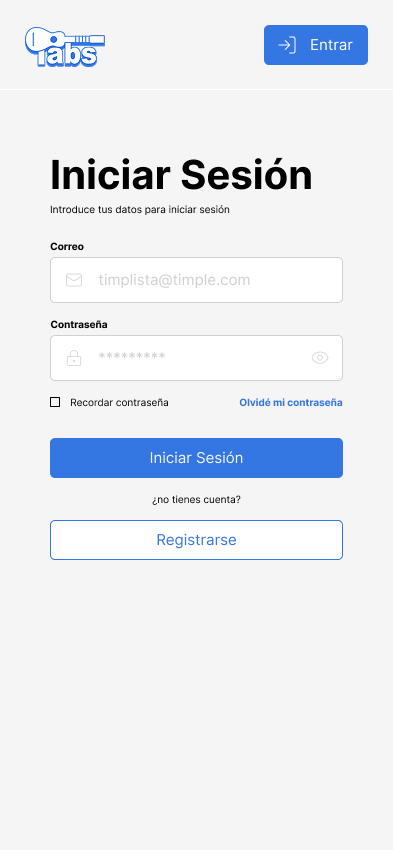
\includegraphics[width=0.8\textwidth]{Ilustraciones/desarrollo/incremento1/diseño/login.jpg}
        \caption{Diseño de página de inicio de sesión}\label{fig:ui_login}
    \end{subfigure}
    \hfill
    \begin{subfigure}[t]{0.3\textwidth}
        \centering
        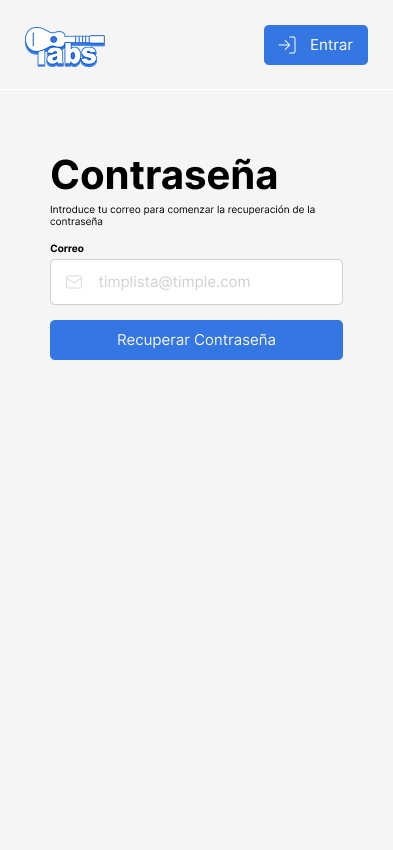
\includegraphics[width=0.8\textwidth]{Ilustraciones/desarrollo/incremento1/diseño/password_recovery.jpg}
        \caption{Diseño de página de recuperación de contraseña}\label{fig:passrec}
    \end{subfigure}
    \hfill
    \begin{subfigure}[t]{0.30\textwidth}
        \centering
        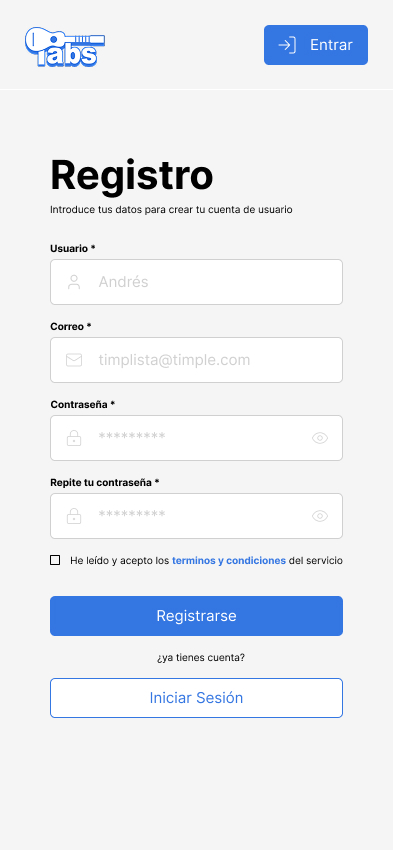
\includegraphics[width=0.8\textwidth]{Ilustraciones/desarrollo/incremento1/diseño/register.jpg}
        \caption{Diseño de pantalla de registro de usuario con campos vacios}\label{fig:ui_register_empty}
    \end{subfigure}
    \hfill
    \begin{subfigure}[t]{0.30\textwidth}
        \centering
        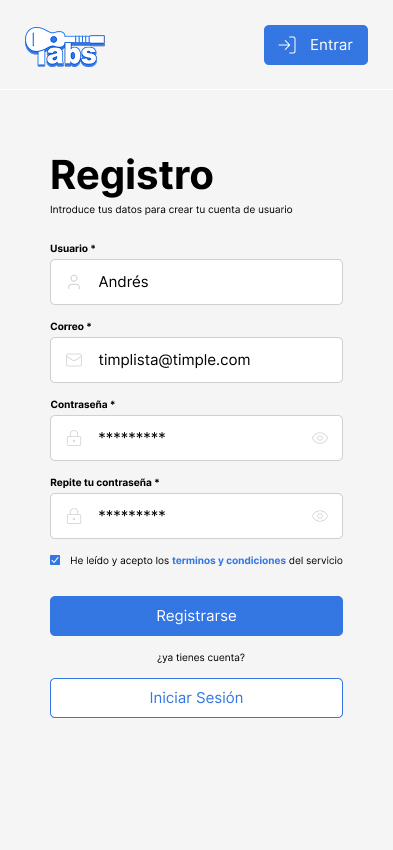
\includegraphics[width=0.8\textwidth]{Ilustraciones/desarrollo/incremento1/diseño/register_filled.jpg}
        \caption{Diseño de pantalla de registro de usuario con campos completados}\label{fig:ui_register_fill}
    \end{subfigure}
    \hfill
    \begin{subfigure}[t]{0.30\textwidth}
        \centering
        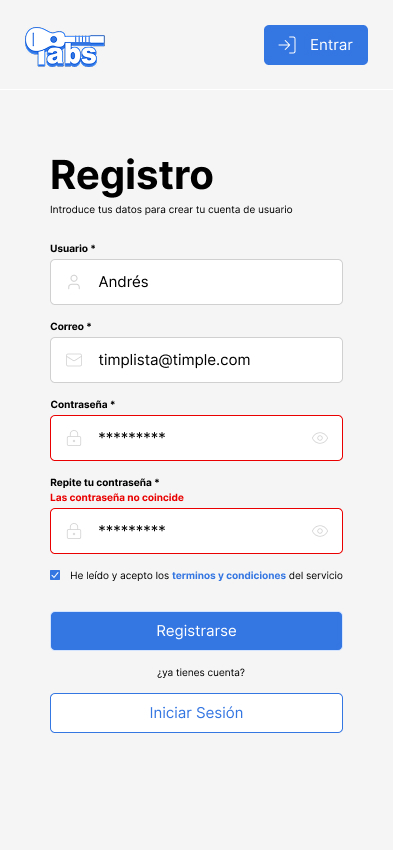
\includegraphics[width=0.8\textwidth]{Ilustraciones/desarrollo/incremento1/diseño/register_error.jpg}
        \caption{Diseño de pantalla de registro de usuario con campos incorrectos}\label{fig:ui_register_fail}
    \end{subfigure}
    \hfill
    \begin{subfigure}[t]{0.3\textwidth}
        \centering
        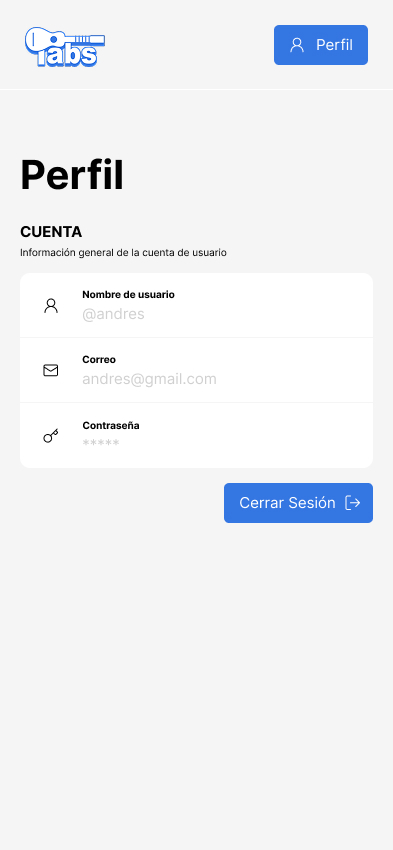
\includegraphics[width=0.8\textwidth]{Ilustraciones/desarrollo/incremento1/diseño/profile.jpg}
        \caption{Diseño de página de perfil de usuario}\label{fig:passrec}
    \end{subfigure}
    \vspace{1em}
    \caption{Diseño de páginas del primer incremento}\label{fig:ui_smt}
\end{figure}

Los anteriores han sido diseñados con el enfoque mobile-first, asegurando una correcta visualización y usabilidad en dispositivos móviles y adaptándose a pantallas de mayor tamaño mediante un diseño responsivo \figref{fig:ui_login_desktop}.

\begin{figure}[H]  
    \centering
    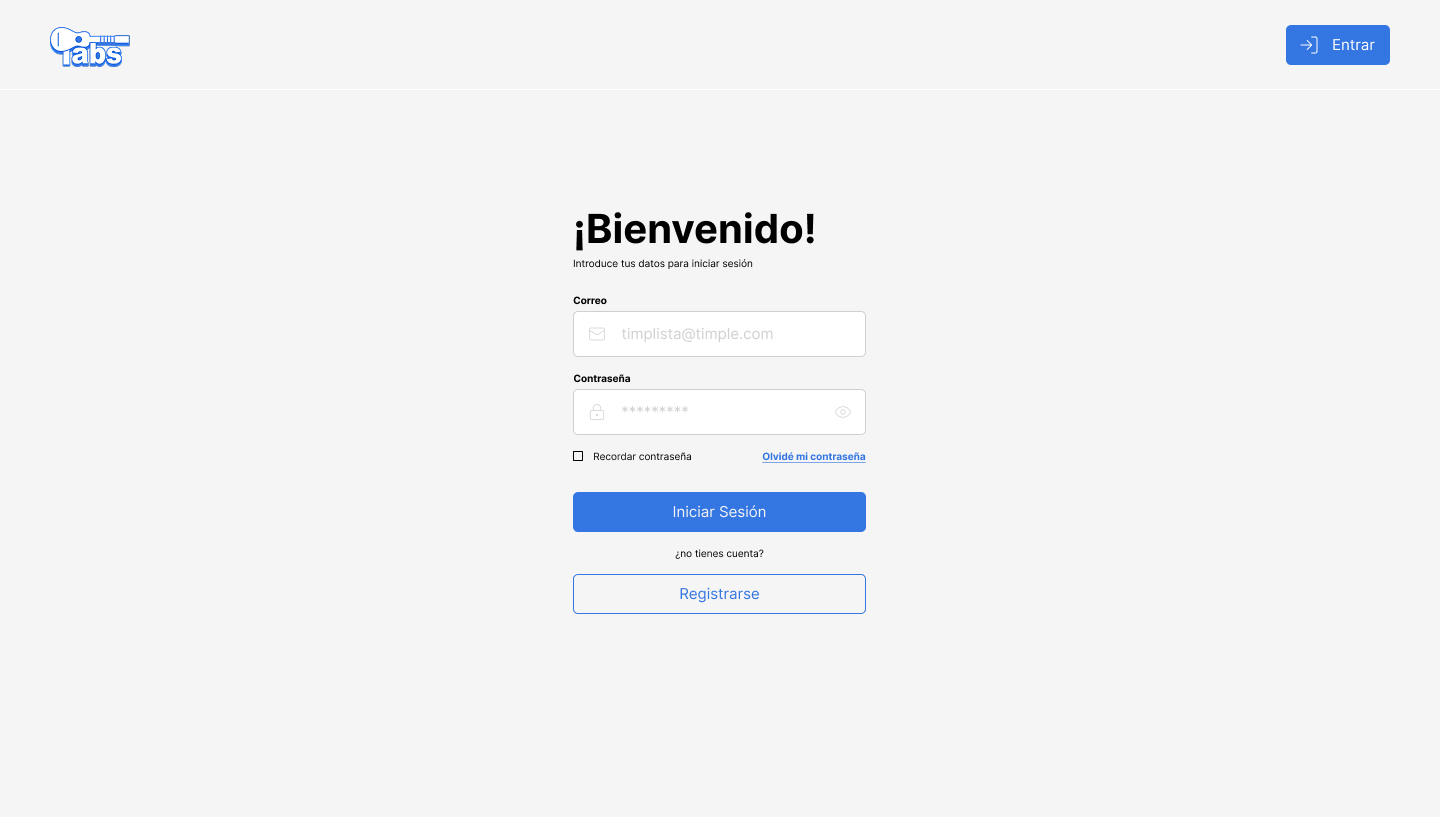
\includegraphics[width=0.8\textwidth]{Ilustraciones/desarrollo/incremento1/diseño/login_big.jpg}
    \caption{Diseño de página de inicio de sesión en pantallas grandes}\label{fig:ui_login_desktop}
\end{figure}

\subsection{Desarrollo}

\chapter{Resultados}
Este capítulo muestra los resultados tras el despliegue del proyecto.
\section{Objetivos cumplidos}

\section{Ajuste a planificación}

\begin{table}[H]
    \caption{Fases, estimación, horas empleadas y tareas.}\label{tab:fases_tareas_ajuste}
    \scriptsize
    \centering
    \begin{tabular}{lll lp{0.45\textwidth}}
        \hline

        \textbf{Fase} & \textbf{Estimación} & \textbf{Empleadas} & \textbf{Tarea} & \textbf{Descripción} \\ \hline
        
        \multirow{2}{*}{Preproducción} 
        & 12h & 8h & 1.1 & Investigación de estado del arte. \\ 
        & 4h & 6h & 1.2 & Selección de tecnologías y herramientas. \\ \hline
        
        \multirow{6}{*}{Desarrollo} 
        & 50h & 80h & 2.1 & Configuración del proyecto, implementación de estructura básica de la web, autenticación y perfil de usuario. \\ 
        & 50h & 32h & 2.2 & Desarrollo de algoritmo de cálculo de acordes. \\ 
        & 50h & act8h & 2.3 & Implementación de páginas para la visualización y creación de publicaciones. \\ 
        & 36h & -- & 2.4 & Desarrollo de biblioteca de publicaciones. \\ 
        & 24h & -- & 2.5 & Implementación de componentes sociales. \\ 
        & 24h & -- & 2.6 & Desarrollo de páginas informativas. \\ \hline
        
        \multirow{2}{*}{Postproducción} 
        & 46h & act40h & 3.1 & Redacción de memoria. \\ 
        & 4h & -- & 3.2 & Elaboración de presentación. \\ \hline
        
    \end{tabular}
\end{table}

\section{Aplicación Web}

\chapter{Manual de usuario}
Este capítulo sirve de orientación para el uso de la aplicación web.

\chapter{Conclusiones}
Este capítulo expone las conclusiones obtenidas sobre todas las fases de desarrollo, así como el producto final.

\bibliography{ref}
\bibliographystyle{IEEEtran}
\clearpage

\printglossaries\end{document}